% Voici le fichier main.tex

\documentclass[12pt,a4paper,oneside]{report}

% ============================================================
% ENCODAGE & LANGUE
% ============================================================
\usepackage{fontspec}
\setmainfont{Calibri}
\usepackage{polyglossia}
\setmainlanguage{french}

\renewcommand{\labelitemi}{\textbullet}
\renewcommand{\labelitemii}{$\circ$}
\renewcommand{\labelitemiii}{$\diamond$}

% ============================================================
% MARGES
% ============================================================
\usepackage{geometry}
\geometry{
	top=3cm,
	bottom=3.5cm,
	left=2.5cm,
	right=2.5cm
}

% ============================================================
% PACKAGES ESSENTIELS
% ============================================================
\usepackage{graphicx}
\usepackage{fancyhdr}
\usepackage{setspace}
\usepackage{titlesec}
\usepackage{tocloft}
\renewcommand{\cftchapleader}{\cftdotfill{\cftdotsep}}
\renewcommand{\cftpartleader}{\cftdotfill{\cftdotsep}}
\usepackage[table]{xcolor}
\usepackage{float}
\usepackage{tikz}
\usepackage{mdframed}
\usepackage{microtype}
\usepackage{array}
\usepackage{booktabs}
\usepackage{etoolbox}
\usepackage{url}
\usepackage{multirow}
\usepackage{chngcntr}

% pour vérifier s'il reste suffisamment d'espace sur la page avant d'écrire le titre de la sous-section
\usepackage{needspace}

% ============================================================
% OUTILS POUR LES RÉFÉRENCES DE PAGE
% ============================================================
\usepackage{refcount} % permet de manipuler les numéros de page pour aider à paginer les Parties dans le Sommaire
\newcommand{\pagerefmoinsun}[1]{%
	\number\numexpr\getpagerefnumber{#1}-1\relax
}

% ============================================================
% LÉGENDES
% ============================================================
\usepackage{caption}

\captionsetup[figure]{name=Figure, labelsep=colon, labelfont={color=vertCongo, bf}, textfont=normalfont}
\captionsetup[table]{name=Tableau, labelsep=colon, labelfont={color=vertCongo, bf}, textfont=normalfont}

\counterwithout{figure}{chapter}
\counterwithout{table}{chapter}

% Format dans la liste : "Figure 1 : " au lieu de "F1"
\renewcommand{\cftfigpresnum}{Figure~}
\renewcommand{\cftfignumwidth}{4.8em}
\renewcommand{\cftfigaftersnum}{ :\ }
\renewcommand{\cfttabpresnum}{Tableau~}
\renewcommand{\cfttabnumwidth}{5.3em}
\renewcommand{\cfttabaftersnum}{ :\ }

% Supprimer les sauts de ligne parasites dans LoF et LoT
\setlength{\cftbeforefigskip}{0pt}
\setlength{\cftbeforetabskip}{2pt}

% ============================================================
% DOSSIER DES IMAGES
% ============================================================

% le principal folder
\graphicspath{{images/}{images/captures_appli/}}

% ============================================================
% COULEURS
% ============================================================
\definecolor{vertCongo}{RGB}{0, 104, 56}
\definecolor{vertFonce}{RGB}{0, 70, 35}
\definecolor{vertClair}{RGB}{220, 240, 228}
\definecolor{jauneCongo}{RGB}{251, 208, 0}
\definecolor{blancPur}{RGB}{255, 255, 255}
\definecolor{grisclair}{RGB}{245, 245, 245}

% ============================================================
% INTERLIGNE
% ============================================================
\onehalfspacing

% ============================================================
% PROFONDEUR DE NUMÉROTATION
% ============================================================
\setcounter{secnumdepth}{3}
\setcounter{tocdepth}{3}

% ============================================================
% ESPACEMENT DES TITRES
% ============================================================
\titlespacing*{\chapter}{0pt}{-20pt}{20pt}
\titlespacing*{\part}{0pt}{0pt}{0pt}

% ============================================================
% FORMAT DES CHAPITRES
% ============================================================
\renewcommand{\thechapter}{\Roman{chapter}}
\renewcommand{\thesection}{\arabic{chapter}.\arabic{section}}
\renewcommand{\thesubsection}{\arabic{chapter}.\arabic{section}.\arabic{subsection}}
\renewcommand{\thesubsubsection}{\arabic{chapter}.\arabic{section}.\arabic{subsection}.\arabic{subsubsection}}

\titleformat{\chapter}[block]
{\normalfont\fontsize{14}{17}\selectfont\bfseries\color{vertCongo}}
{Chapitre~\thechapter~:}
{1em}
{}

\titleformat{\section}
{\normalfont\fontsize{12}{15}\selectfont\bfseries\color{vertCongo}}
{\thesection}
{1em}
{}

\titleformat{\subsection}
{\normalfont\fontsize{12}{15}\selectfont\bfseries\color{vertCongo}}
{\thesubsection}
{1em}
{}

\titleformat{\subsubsection}
{\normalfont\fontsize{12}{15}\selectfont\bfseries\color{vertCongo}}
{\thesubsubsection}
{1em}
{}

% Titres des chapitres spéciaux (Dédicace, Remerciements, etc.) en vertCongo
\titleformat{name=\chapter,numberless}[block]
{\normalfont\fontsize{14}{17}\selectfont\bfseries\color{vertCongo}}
{}
{0em}
{}

% Forcer la taille 14pt sur les titres auto (Liste des figures, etc.)
\patchcmd{\listoffigures}{\chapter*}{\chapter*}{}{}
\renewcommand{\cftloftitlefont}{\normalfont\fontsize{14}{17}\selectfont\bfseries\color{vertCongo}}
\renewcommand{\cftlottitlefont}{\normalfont\fontsize{14}{17}\selectfont\bfseries\color{vertCongo}}
\renewcommand{\cfttoctitlefont}{\normalfont\fontsize{14}{17}\selectfont\bfseries\color{vertCongo}}

% Réduire l'espace entre le titre et le contenu
\setlength{\cftbeforetoctitleskip}{-20pt}
\setlength{\cftbeforeloftitleskip}{-20pt}
\setlength{\cftbeforelottitleskip}{-20pt}
\setlength{\cftaftertoctitleskip}{6pt}
\setlength{\cftafterloftitleskip}{10pt}
\setlength{\cftafterlottitleskip}{10pt}

% Pour mettre "Table des matières avec une taille de police pareille à Annexes et Bibliographie"
\renewcommand{\cfttoctitlefont}{\normalfont\fontsize{14}{17}\selectfont\bfseries\color{vertCongo}}

% Pour supprimer l'espace verticale avant LoT, LoF, et ToC
\setlength{\cftbeforetoctitleskip}{-20pt}
\setlength{\cftbeforeloftitleskip}{-20pt}
\setlength{\cftbeforelottitleskip}{-20pt}

% ============================================================
% TABLE DES MATIÈRES — personnalisation
% ============================================================

% SECTIONS : 16pt gras (plus grand que les Parties)
% Injectées via \addtocontents, pas via \part

% PARTIES : 14pt gras — style de l'entrée "part" dans la TDM
\renewcommand{\cftpartfont}{\fontsize{13}{16}\selectfont\bfseries}
\renewcommand{\cftpartpagefont}{\fontsize{13}{16}\selectfont\bfseries}
\setlength{\cftbeforepartskip}{8pt}
\setlength{\cftpartindent}{1cm}        % légère indentation sous la Section

% CHAPITRES : 12pt gras, indentés sous les Parties
\renewcommand{\cftchappresnum}{Chapitre~}
\setlength{\cftchapnumwidth}{5em}
\setlength{\cftchapindent}{2cm}        % indentés sous les Parties
\renewcommand{\cftchapfont}{\fontsize{12}{15}\selectfont\bfseries}
\renewcommand{\cftchappagefont}{\fontsize{12}{15}\selectfont\bfseries}
\setlength{\cftbeforechapskip}{3pt}

% SECTIONS (1.1, 1.2...) : indentées sous les chapitres
\setlength{\cftsecindent}{3.5cm}
\renewcommand{\cftsecfont}{\fontsize{12}{15}\selectfont}
\renewcommand{\cftsecpagefont}{\fontsize{12}{15}\selectfont}
\setlength{\cftbeforesecskip}{1pt}

% SOUS-SECTIONS (1.1.1...)
\setlength{\cftsubsecindent}{4.5cm}
\renewcommand{\cftsubsecfont}{\fontsize{12}{15}\selectfont}
\renewcommand{\cftsubsecpagefont}{\fontsize{12}{15}\selectfont}

% SOUS-SOUS-SECTIONS (1.1.1.1...)
\setlength{\cftsubsubsecindent}{5.5cm}
\renewcommand{\cftsubsubsecfont}{\fontsize{12}{15}\selectfont}
\renewcommand{\cftsubsubsecpagefont}{\fontsize{12}{15}\selectfont}

% ============================================================
% EN-TÊTE ET PIED DE PAGE
% ============================================================
\setlength{\headheight}{40pt}
\setlength{\footskip}{40pt}

\newcommand{\enteteContenu}{%
	\small\bfseries
	Conception et réalisation d'une application cross-plateforme de mise en relation entre prestataires et clients pour services professionnels à Akieni
}
\newcommand{\piedContenu}{%
	\small
	Grâce Deo BATA \& Christophe Darly MASSAMBA BOUESSO\\
	LP-GL \textbar{} 2025-2026
}

\fancypagestyle{styleGlobal}{
	\fancyhf{}
	\fancyhead[C]{\enteteContenu}
	\fancyfoot[L]{\piedContenu}
	\fancyfoot[R]{\small\thepage}
	\renewcommand{\headrulewidth}{0.4pt}
	\renewcommand{\footrulewidth}{0.4pt}
}

\fancypagestyle{plain}{
	\fancyhf{}
	\fancyhead[C]{\enteteContenu}
	\fancyfoot[L]{\piedContenu}
	\fancyfoot[R]{\small\thepage}
	\renewcommand{\headrulewidth}{0.4pt}
	\renewcommand{\footrulewidth}{0.4pt}
}

\fancypagestyle{styleSansPagination}{
	\fancyhf{}
	\fancyhead[C]{\enteteContenu}
	\fancyfoot[L]{\piedContenu}
	\renewcommand{\headrulewidth}{0.4pt}
	\renewcommand{\footrulewidth}{0.4pt}
}

% ============================================================
% PAGE D'ANNONCE DE SECTION
% ============================================================
\newcommand{\pageSectionAnnonce}[1]{%
	\clearpage
	\thispagestyle{styleSansPagination}
	\vspace*{\fill}
	\begin{center}
		\begin{tikzpicture}
			\node[
			fill=vertCongo,
			text=blancPur,
			font=\Huge\bfseries,
			minimum width=14cm,
			minimum height=3.5cm,
			rounded corners=8pt,
			inner sep=16pt,
			align=center
			] {#1};
		\end{tikzpicture}
	\end{center}
	\vspace*{\fill}
	\clearpage
}

% ============================================================
% PAGE D'ANNONCE DE PARTIE (taille 16pt)
% ============================================================
\newcommand{\pagePartieAnnonce}[3]{%
	\clearpage
	\phantomsection
	\addcontentsline{toc}{part}{#3}%
	\thispagestyle{styleSansPagination}
	\vspace*{\fill}
	\begin{center}
		\begin{tikzpicture}
			\node[
			fill=vertCongo,
			text=blancPur,
			font=\fontsize{16}{20}\selectfont\bfseries,
			minimum width=13cm,
			minimum height=2.8cm,
			rounded corners=6pt,
			inner sep=14pt,
			align=center
			] {#1\\[4pt]\normalsize\mdseries #2};
		\end{tikzpicture}
	\end{center}
	\vspace*{\fill}
	\clearpage
}

% ============================================================
% HYPERREF — toujours en dernier
% ============================================================
\usepackage{hyperref}
\hypersetup{
	colorlinks=false,
	pdfborder={0 0 0},
	pdftitle={Rapport SALISA - LP Génie Logiciel},
	pdfauthor={Grâce Deo BATA, Christophe Darly MASSAMBA BOUESSO}
}

% ============================================================
% GESTION DES COUPURES DE MOTS
% ============================================================
\usepackage[none]{hyphenat}
\sloppy
\setlength{\emergencystretch}{3em}

% ============================================================
% AJOUT DE LA MARGE (DÉCALAGE DANS LES REMERCIEMENTS)
% ============================================================
%\usepackage{scrextend}


% ============================================================
% GESTION DES PUCES
% ============================================================
\usepackage{enumitem}


% ============================================================
% GESTION DE COULEUR DE POLICE VERTCONGO
% ============================================================
\renewcommand{\listfigurename}{Liste des figures}
\renewcommand{\listtablename}{Liste des tableaux}

% ============================================================
%                        DOCUMENT
% ============================================================
\begin{document}
	
	\pagestyle{styleGlobal}
	
	% ============================================================
	% SECTION I
	% ============================================================
	\pageSectionAnnonce{SECTION I}
	\pagenumbering{Roman}
	\addtocontents{toc}{%
		\vspace{6pt}%
		\noindent{\fontsize{13}{16}\selectfont\bfseries SECTION I}\par%
		\vspace{3pt}%
	}
	
	% ============================================================
% DEDICACE
% ============================================================
\chapter*{Dédicace}
\pagestyle{styleGlobal}
\label{sec:dedicace}
\markboth{Dédicace}{Dédicace}
\addcontentsline{toc}{chapter}{Dédicace}

\begin{center}
	\itshape
	
	À mes parents,
	votre dévouement sans limites est la raison de ce jour.\\[0.2cm]
	
	À mon oncle,
	merci pour chaque conseil, chaque orientation, chaque mot juste.\\[0.2cm]
	
	À mes frères et sœurs,
	votre amour et votre foi en moi ont tout changé.\\[0.2cm]
	
\end{center}

\vspace{0.8cm}
\begin{flushright}
	\textbf{Grâce Deo BATA}
\end{flushright}

\vspace*{1cm}
\noindent\rule{\textwidth}{0.4pt}
\vspace*{1cm}

\begin{center}
	\itshape
	
	À mes parents, 
	pour leur amour, leur soutien indéfectible\\ 
	et les sacrifices consentis
	tout au long de ce parcours.\\[0.2cm]
	
	À tous ceux et toutes celles qui ont cru en mon potentiel\\
	bien avant que je ne le découvre moi-même, leur clairvoyance avait vu juste.
	
\end{center}

\vspace{0.8cm}
\begin{flushright}
	\textbf{Christophe Darly MASSAMBA BOUESSO}
\end{flushright}
	\newpage
	
	% ============================================================
% REMERCIEMENTS
% ============================================================
\chapter*{Remerciements}
\pagestyle{styleGlobal}
\label{sec:remerciements}
\markboth{Remerciements}{Remerciements}
\addcontentsline{toc}{chapter}{Remerciements}

\vspace*{1cm}

Nous tenons à exprimer notre profonde gratitude à toutes les personnes qui ont contribué, de près ou de loin, à la réalisation de ce travail.

Nos remerciements vont en premier lieu à notre Directeur de Projet, M. Ornel Djenifer KIGOMA, ingénieur informaticien et enseignant à l'ESGAE, pour sa disponibilité, ses orientations pertinentes et sa rigueur tout au long de l'encadrement de ce projet. Ses conseils ont été déterminants dans la qualité du travail produit.

Nous remercions également l'ensemble du corps enseignant et administratif de l'École Supérieure de Gestion et d'Administration des Entreprises (ESGAE) de Brazzaville pour la formation dispensée durant ces années de Licence Professionnelle en Génie Logiciel.

Nos remerciements vont aussi à la structure Akieni, qui nous a fourni les informations nécessaires à la réalisation de ce projet, et plus particulièrement à M. Grâce Deo BATA pour sa connaissance de la structure et le lien qu'il a su établir entre notre travail et la réalité du terrain.

Enfin, nous remercions nos familles respectives pour leur soutien moral et matériel constant, sans lequel ce parcours n'aurait pas été possible.
	\newpage
	
	\phantomsection
	\label{sec:figures}
	\addcontentsline{toc}{chapter}{Liste des figures}
	\renewcommand{\listfigurename}{\textcolor{vertCongo}{Liste des figures}}
	\listoffigures
	\newpage
	
	\phantomsection
	\label{sec:tableaux}
	\addcontentsline{toc}{chapter}{Liste des tableaux}
	\renewcommand{\listtablename}{\textcolor{vertCongo}{Liste des tableaux}}
	\listoftables
	\newpage
	
	% ============================================================
% ABREVIATIONS ET SIGLES
% ============================================================
\chapter*{Abréviations et Sigles}
\pagestyle{styleGlobal}
\label{sec:abreviations}
\markboth{Abréviations et Sigles}{Abréviations et Sigles}
\addcontentsline{toc}{chapter}{Abréviations et Sigles}

\begin{table}[H]
	\caption{Liste des abréviations et sigles utilisés}
	\label{tab:abreviations}
	\centering
	\begin{tabular}{|p{3.2cm}|p{10cm}|}
		\hline
		\rowcolor{vertCongo}
		\textcolor{white}{\textbf{Abrév. / Sigles}} & \textcolor{white}{\textbf{Signification}} \\
		\hline
		\textbf{ESGAE}  & École Supérieure de Gestion et d'Administration des Entreprises \\[3pt]
		\hline
		\textbf{API}    & Application Programming Interface \\[3pt]
		\hline
		\textbf{FCFA}   & Franc de la Coopération Financière en Afrique centrale \\[3pt]
		\hline
		\textbf{HTTP}   & HyperText Transfer Protocol \\[3pt]
		\hline
		\textbf{IA}     & Intelligence Artificielle \\[3pt]
		\hline
		\textbf{JWT}    & JSON Web Token \\[3pt]
		\hline
		\textbf{LP-GL}  & Licence Professionnelle - Génie Logiciel \\[3pt]
		\hline
		\textbf{MoMo}   & Mobile Money \\[3pt]
		\hline
		\textbf{MTN}    & Mobile Telephone Network \\[3pt]
		\hline
		\textbf{SMS}    & Short Message Service \\[3pt]
		\hline
		\textbf{OTP}    & One-Time Password \\[3pt]
		\hline
		\textbf{PWA}    & Progressive Web Application \\[3pt]
		\hline
		\textbf{REST}   & Representational State Transfer \\[3pt]
		\hline
		\textbf{BD}     & Base de Données \\[3pt]
		\hline
		\textbf{SGBD}   & Système de Gestion de Bases de Données \\[3pt]
		\hline
		\textbf{SQL}    & Structured Query Language \\[3pt]
		\hline
		\textbf{UML}    & Unified Modeling Language \\[3pt]
		\hline
		\textbf{UP}     & Unified Process (Processus Unifié) \\[3pt]
		\hline
		\textbf{2TUP}   & Two Tracks Unified Process \\[3pt]
		\hline
		\textbf{UC}     & Use Case (Cas d'utilisation) \\[3pt]
		\hline
		\textbf{RG}     & Règle de Gestion \\[3pt]
		\hline
		\textbf{URL}    & Uniform Resource Locator \\[3pt]
		\hline
		\textbf{WSS}    & WebSocket Secure \\[3pt]
		\hline
	\end{tabular}
\end{table}
	\newpage
	
	% ============================================================
% SOMMAIRE - Grands titres uniquement
% ============================================================
\chapter*{Sommaire}
\pagestyle{styleGlobal}
\markboth{Sommaire}{Sommaire}
\addcontentsline{toc}{chapter}{Sommaire}

% Ligne normale : Titre ........ page
\newcommand{\lignesom}[2]{%
    \noindent #1\dotfill\textbf{#2}\par\addvspace{4pt}%
}

% Ligne indentée (chapitres sous les parties)
\newcommand{\lignesomindent}[2]{%
    \noindent\hspace{1cm}#1\dotfill\textbf{#2}\par\addvspace{4pt}%
}

\vspace{0.6cm}

% ---- SECTION I ----
\noindent\textbf{\large SECTION I}

\vspace{0.4cm}

\lignesom{Dédicace}{\pageref{sec:dedicace}}
\lignesom{Remerciements}{\pageref{sec:remerciements}}
\lignesom{Liste des figures}{\pageref{sec:figures}}
\lignesom{Liste des tableaux}{\pageref{sec:tableaux}}
\lignesom{Abréviations et sigles}{\pageref{sec:abreviations}}

\vspace{0.7cm}

% ---- SECTION II ----
\noindent\textbf{\large SECTION II}

\vspace{0.4cm}

\lignesom{Introduction}{\pageref{sec:introduction}}

\vspace{0.3cm}
\noindent\textbf{Première Partie : Présentation Générale}

\vspace{0.2cm}
\lignesomindent{Chapitre I : La structure d'accueil et le sujet}{\pageref{chap:structure_sujet}}

\vspace{0.3cm}
\noindent\textbf{Deuxième Partie : Analyse et Conception}

\vspace{0.2cm}
\lignesomindent{Chapitre I : Étude préliminaire et Méthode}{\pageref{chap:etude_preliminaire}}
\lignesomindent{Chapitre II : Analyse et Conception}{\pageref{chap:analyse_conception}}

\vspace{0.3cm}
\noindent\textbf{Troisième Partie : Évaluation et Réalisation du Projet}

\vspace{0.2cm}
\lignesomindent{Chapitre I : L'évaluation du projet}{\pageref{chap:evaluation}}
\lignesomindent{Chapitre II : Les outils et les techniques utilisés}{\pageref{chap:outils}}

\vspace{0.2cm}
\lignesom{Conclusion}{\pageref{sec:conclusion}}

\vspace{0.7cm}

% ---- SECTION III ----
% La table des matières s'étend sur les pages a, b, c
% La bibliographie commence à la page d
% Les annexes commencent à la page e
\noindent\textbf{\large SECTION III}

\vspace{0.4cm}

\lignesom{Table des matières}{\pageref{sec:tabledesmatieres}}
\lignesom{Bibliographie}{\pageref{sec:bibliographie}}
\lignesom{Annexes}{\pageref{sec:annexes}}

	\newpage
	
	% ============================================================
	% SECTION II
	% ============================================================
	\pageSectionAnnonce{SECTION II}
	\pagenumbering{arabic}
	\addtocontents{toc}{%
		\vspace{10pt}%
		\noindent{\fontsize{13}{16}\selectfont\bfseries SECTION II}\par%
		\vspace{3pt}%
	}
	
	% ============================================================
% INTRODUCTION
% ============================================================
\chapter*{Introduction}
\pagestyle{styleGlobal}
\label{sec:introduction}
\markboth{Introduction}{Introduction}
\addcontentsline{toc}{chapter}{Introduction}

Le numérique a changé la façon dont les personnes accèdent aux services professionnels. Aujourd'hui, des plateformes numériques permettent de trouver facilement un professionnel compétent pour réaliser une tâche précise, de consulter son profil, de le contacter et de le payer en toute sécurité. Cependant, dans bien des environnements, cette mise en relation entre prestataires et clients reste informelle, peu structurée et difficile à organiser. C'est dans ce contexte qu'Akieni, société spécialisée dans la transformation digitale au Congo, a exprimé le besoin de disposer d'une solution numérique capable de connecter de manière fiable des prestataires de services professionnels avec des clients. C'est ainsi qu'est né «~SALISA~», notre solution pour répondre directement à ce besoin.

La problématique principale de ce travail peut être formulée ainsi : comment concevoir et réaliser une application cross-plateforme qui permet de connecter efficacement des prestataires et des clients, en garantissant la qualité des services, la sécurité des transactions et une expérience simple pour tous les utilisateurs ?

Pour répondre à cette problématique, nous formulons les hypothèses suivantes. Premièrement, un système de vérification d'identité et de notation permettra d'établir la confiance entre les utilisateurs de la plateforme. Deuxièmement, un algorithme de mise en correspondance basé sur les compétences, la localisation et le budget aidera les clients à trouver rapidement le bon prestataire. Troisièmement, l'intégration du paiement Mobile Money avec un mécanisme de sécurisation des fonds (escrow) protégera les deux parties lors des transactions. Quatrièmement, l'utilisation du processus 2TUP combiné au langage de modélisation UML permettra de concevoir un système solide et bien structuré.

Ce travail s'intitule : \textbf{«~Conception et réalisation d'une application cross-plateforme de mise en relation entre prestataires et clients pour services professionnels à Akieni~»}. Il est organisé en trois grandes parties. La première présente la structure d'accueil Akieni ainsi que le cadrage général du travail. La deuxième est consacrée à l'analyse des besoins et à la conception du système selon la démarche 2TUP et UML. La troisième décrit les outils utilisés, le planning et les résultats obtenus.

	\newpage
	
	% ---- PREMIERE PARTIE ----
	\pagePartieAnnonce%
	{Première Partie}%
	{PRÉSENTATION GÉNÉRALE}%
	{Première Partie : Présentation Générale}
	\setcounter{chapter}{0}
	
	% ============================================================
% PARTIE I - CHAPITRE I : La structure d'accueil et le sujet
% ============================================================
\chapter{La structure d'accueil et le sujet}
\pagestyle{styleGlobal}
\label{chap:structure_sujet}

% ============================================================
\section{La structure d'accueil}
% ============================================================

\subsection{Historique}

Akieni est une société spécialisée dans la transformation numérique et les solutions logicielles en République du Congo. Implantée à Brazzaville depuis 2022, elle a pour mission d'accompagner les entreprises et les institutions publiques et privées dans leurs projets de transformation digitale. Elle est reconnue comme un acteur majeur du numérique et collabore avec des gouvernements, des institutions, des entreprises et des citoyens à travers l’Afrique centrale. 

Parmi ses initiatives, Akieni a lancé le programme de formation \textit{Akieni Academy}, dont la première promotion a démarré officiellement le 15 novembre 2024 à Brazzaville. À cette occasion, 120 apprenants ont été sélectionnés parmi 1 740 candidats présélectionnés en ligne, venant du Congo, du Cameroun, du Rwanda et de la République Démocratique du Congo. La deuxième promotion a été lancée en janvier 2026, avec l'ambition de former 400 nouveaux apprenants. L'objectif à long terme d'Akieni est de former 30 000 jeunes aux métiers du numérique d'ici 2030, afin de positionner le Congo comme un pôle d'exportation de compétences digitales. La structure est dirigée par M. Frédéric NZÉ, actuel Ministre des Postes, des Télécommunications et de l'Économie numérique de la République du Congo.

\subsection{Missions}

Akieni a plusieurs missions principales :

\begin{itemize}
	\item accompagner les organisations publiques et privées dans leurs projets de transformation digitale ;
	\item promouvoir les talents locaux et organiser des événements numériques tels que des hackathons pour encourager l'innovation ;
	
	\item investir dans le capital humain ;
	\item stimuler la transformation par la collaboration ;
	\item favoriser l'innovation numérique.
\end{itemize}

\subsection{Organigramme Général}

La figure~\ref{fig:organigramme_akieni} présente l'organisation générale d'Akieni, structurée autour d'une Direction Générale qui supervise cinq directions principales, chacune pilotant ses propres départements opérationnels.

\begin{figure}[H]
	\centering
	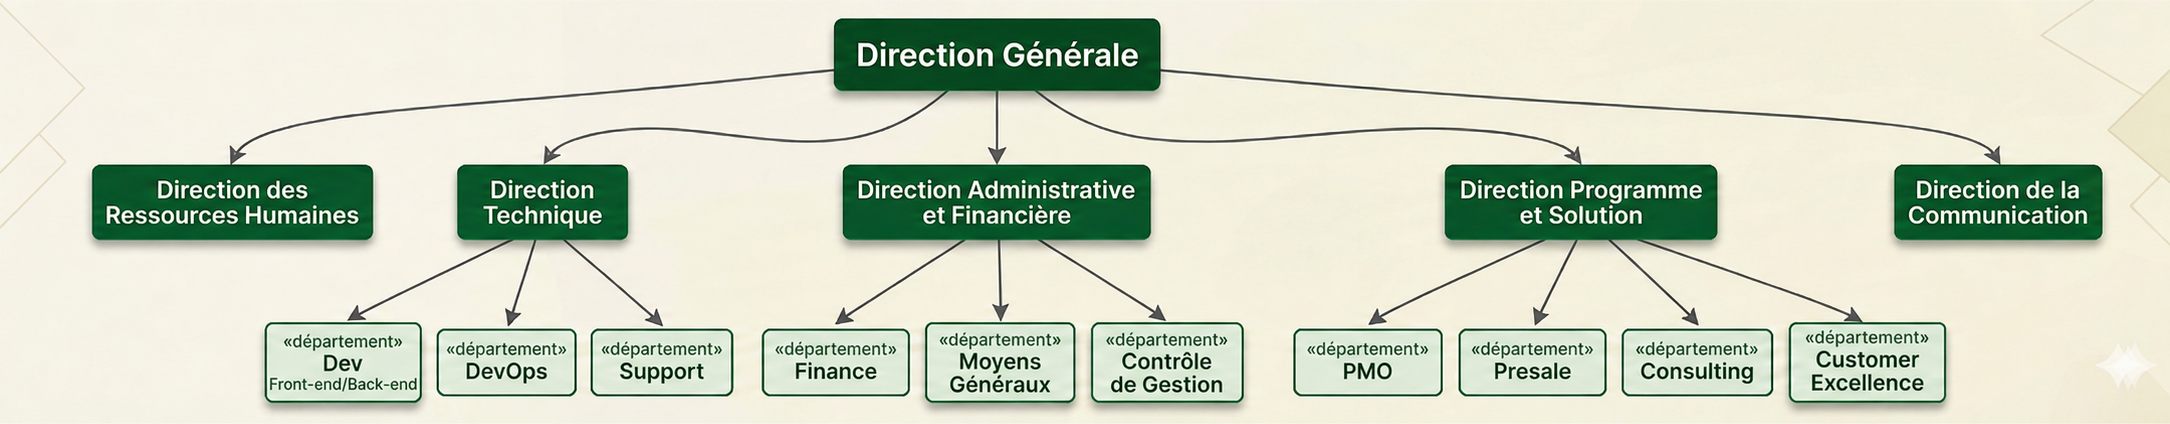
\includegraphics[width=0.95\textwidth]{organigramme_akieni.png}
	\caption{Organigramme général d'Akieni}
	\label{fig:organigramme_akieni}
\end{figure}

\subsection{Attributions des structures}

Akieni est organisée en cinq directions principales, chacune ayant un domaine de responsabilité bien défini.

\textbf{La Direction des Ressources Humaines} gère le recrutement, la gestion des carrières et le bien-être du personnel. Elle veille à ce que les équipes disposent des compétences nécessaires pour mener à bien les projets de la structure.

\textbf{La Direction Technique} est le cœur opérationnel d'Akieni sur le plan technologique. Elle regroupe trois départements : le département de développement Front-end et Back-end, qui conçoit et maintient les applications et plateformes numériques ; le département DevOps, qui assure l'intégration continue, le déploiement et la supervision des infrastructures ; et le département Support, qui gère l'assistance technique auprès des utilisateurs internes et des clients.

\textbf{La Direction Administrative et Financière} assure la gestion des ressources financières et administratives de la structure. Elle comprend le département Finance, chargé de la comptabilité et du suivi budgétaire ; le département Moyens Généraux, qui gère les équipements et les locaux ; et le département Contrôle de Gestion, qui évalue la performance financière de l'organisation.

\textbf{La Direction Programme et Solution} pilote les projets clients et les offres de services d'Akieni. Elle s'appuie sur quatre départements : le PMO (\textit{Project Management Office}), qui coordonne et standardise la gestion des projets ; le département Presale, qui accompagne les avant-ventes et la rédaction des offres commerciales ; le département Consulting, qui propose des conseils en transformation numérique ; et le département Customer Excellence, qui veille à la satisfaction client et à l'excellence de la qualité des livrables.

\textbf{La Direction de la Communication} est responsable de la communication interne et externe de la structure, de la gestion de l'image de marque d'Akieni, ainsi que de la promotion de ses programmes et de ses offres auprès du grand public et des partenaires.

\subsection{Situation informatique}

\subsubsection{Personnel informatique}

Akieni étant une structure spécialisée dans le numérique, l'essentiel de son personnel est à profil technique. L'équipe informatique est rattachée à la Direction Technique et se compose notamment de développeurs Full Stack (Front-end et Back-end), d'ingénieurs DevOps chargés de l'infrastructure et du déploiement, et de techniciens support. La Direction Programme et Solution compte également des consultants et des chefs de projet qui encadrent les missions techniques chez les clients.

\subsubsection{Matériels informatiques}

Pour mener ses activités de formation, de développement et de conseil, Akieni dispose d'un parc matériel adapté à ses besoins. On y trouve notamment des postes de travail et des ordinateurs portables mis à disposition des équipes techniques et des apprenants, des serveurs locaux utilisés pour les environnements de développement et de test, ainsi que les équipements réseau nécessaires à la connectivité de ses locaux (routeurs, switchs, points d'accès Wi-Fi). Les projections et présentations en salle de formation sont assurées par des vidéoprojecteurs et des écrans interactifs.

\subsubsection{Logiciels informatiques}

Akieni utilise un ensemble d'outils logiciels couvrant ses différents besoins. Sur le plan du développement, les équipes travaillent avec des environnements tels que Visual Studio Code, Git et GitHub pour la gestion du code source, ainsi que des plateformes cloud comme AWS ou Azure pour l'hébergement des applications. Pour la gestion de projets, des outils comme Jira ou Trello sont utilisés au sein du PMO. La communication interne repose sur des solutions telles que Slack ou Microsoft Teams. Enfin, les formations de l'Akieni Academy s'appuient sur des plateformes d'apprentissage en ligne (LMS) permettant de suivre la progression des apprenants à distance.

% ============================================================
\section{Le sujet}
% ============================================================

\subsection{Contexte du sujet}

Le numérique occupe aujourd'hui une place centrale dans l'organisation des services professionnels. Les plateformes numériques ont remplacé progressivement les méthodes traditionnelles de recherche de prestataires, offrant plus de transparence et d'efficacité. Cependant, à Brazzaville, de nombreux professionnels exercent dans des domaines variés comme l'artisanat, les services techniques, les prestations intellectuelles ou les services à la personne, mais ils restent peu visibles faute d'une plateforme numérique adaptée.

De leur côté, les particuliers, les entreprises et les institutions ont du mal à trouver rapidement un prestataire compétent, disponible et de confiance. Les échanges reposent encore largement sur le bouche-à-oreille, sans aucune garantie de qualité ni de sécurité financière.

« SALISA » naît de ce constat. Il s'agit d'une application cross-plateforme conçue pour faciliter la mise en relation entre prestataires et clients, en intégrant un système de vérification des profils, un mécanisme de paiement sécurisé et un outil de notation des prestations. Le nom \textit{SALISA}, emprunté au lingala, a une double signification : pour le prestataire, \textit{ko salisa} signifie \textit{"aider"} et pour le demandeur, \textit{salisa} signifie \textit{"faire faire"} (un travail).

\subsection{Problématique du sujet}

Malgré la présence de nombreux prestataires de services à Brazzaville, il n'existe pas de mécanisme fiable permettant de les mettre en relation avec les clients. Les échanges se font de façon informelle, sans garantie de qualité, de ponctualité ni de sécurité financière pour les parties concernées.

La problématique principale de ce travail peut être formulée ainsi :

\begin{center}
	\itshape
	Comment concevoir et mettre en \oe{}uvre une application cross-plateforme efficace permettant de connecter des prestataires et des clients, tout en garantissant la fiabilité des services, la sécurité des transactions et une expérience utilisateur adaptée au contexte local ?
\end{center}

Cette problématique soulève plusieurs enjeux : la gestion de la confiance entre utilisateurs, l'optimisation du choix des prestataires grâce à un mécanisme de mise en correspondance intelligent, la sécurisation des paiements, et l'accessibilité de la solution sur des appareils variés.

\subsection{Intérêts du sujet}

L'intérêt de ce travail se situe à plusieurs niveaux.

\begin{itemize}
	\item[\textbf{-}] \textbf{Sur le plan économique :} la plateforme permet de dynamiser le marché des services en facilitant l'accès aux opportunités pour les prestataires et en réduisant les difficultés de recherche pour les clients. Elle contribue à la création de valeur économique locale et à l'insertion professionnelle.
	
	\item[\textbf{-}] \textbf{Sur le plan social :} « SALISA » favorise l'inclusion numérique en offrant à un large public la possibilité d'accéder à des services fiables et de faire connaître leurs compétences. Elle encourage également les transactions formelles entre citoyens.
	
	\item[\textbf{-}] \textbf{Sur le plan technologique :} le travail intègre des solutions modernes comme la mise en correspondance intelligente (matching), la géolocalisation par quartier et le paiement mobile via MTN MoMo et Airtel Money, ce qui renforce sa pertinence dans un contexte numérique en développement.
	
	\item[\textbf{-}] \textbf{Sur le plan académique :} ce travail est une application concrète des enseignements du génie logiciel, notamment l'analyse des besoins, la modélisation UML, la conception de systèmes distribués et le développement d'applications selon la démarche \textbf{2TUP}.
\end{itemize}

% ============================================================
\section{Concepts liés au sujet}

La compréhension de ce travail nécessite la maîtrise de plusieurs concepts clés, définis ci-après.

\begin{itemize}
	\item[\textbf{-}] \textbf{Application cross-plateforme :} désigne une application conçue pour fonctionner sur plusieurs types de terminaux et de systèmes d'exploitation (web, Android, iOS) à partir d'une seule base de code, ce qui réduit les coûts et les délais de développement.
	
	\item[\textbf{-}] \textbf{Mise en relation :} processus qui consiste à connecter une offre de service proposée par un prestataire à une demande exprimée par un client, en s'appuyant sur des critères de compatibilité définis.
	
	\item[\textbf{-}] \textbf{Matching :} mécanisme qui identifie automatiquement les prestataires les plus adaptés à une demande, en tenant compte des compétences, de la localisation géographique, de la disponibilité, du budget et des évaluations reçues.
	
	\item[\textbf{-}] \textbf{Système de confiance :} ensemble de mécanismes tels que les notes, les avis, la vérification d'identité et les badges de certification, qui permettent de s'assurer de la fiabilité des utilisateurs et de la qualité des services proposés.
	
	\item[\textbf{-}] \textbf{Paiement mobile :} solution de paiement électronique très utilisée en Afrique, qui permet d'effectuer des transactions financières via un téléphone mobile, sans avoir besoin d'un compte bancaire. Au Congo, les deux opérateurs de paiement mobile sont MTN MoMo et Airtel Money.
	
	\item[\textbf{-}] \textbf{API (Application Programming Interface) :} interface de programmation qui permet à deux applications de communiquer entre elles en échangeant des données selon un protocole défini. Dans le cadre de « SALISA », les API de MTN MoMo et d'Airtel Money sont utilisées pour intégrer le paiement mobile directement dans la plateforme.
	
	\item[\textbf{-}] \textbf{Progressive Web Application (PWA) :} application web qui offre une expérience proche d'une application mobile classique, avec un fonctionnement possible hors connexion, l'installation sur l'écran d'accueil et des notifications. Elle ne nécessite pas de téléchargement depuis un store d'applications.
	
	\item[\textbf{-}] \textbf{UML (Unified Modeling Language) :} langage de modélisation graphique utilisé en génie logiciel pour représenter les différents aspects d'un système informatique, comme les cas d'utilisation, les classes, les séquences ou le déploiement.
	
	\item[\textbf{-}] \textbf{2TUP (Two Tracks Unified Process) :} processus de développement logiciel dérivé du Processus Unifié (UP), qui organise la conception selon deux axes parallèles : la branche fonctionnelle (besoins métier) et la branche technique (contraintes d'architecture), qui fusionnent en phase de réalisation.
	
	\item[\textbf{-}] \textbf{Géolocalisation :} technique qui permet de situer un utilisateur ou un service dans un espace géographique, afin de faciliter la mise en relation de proximité entre prestataires et clients.
\end{itemize}
	
	% ---- DEUXIEME PARTIE ----
	\pagePartieAnnonce%
	{Deuxième Partie}%
	{ANALYSE ET CONCEPTION}%
	{Deuxième Partie : Analyse et Conception}
	\setcounter{chapter}{0}
	
	% ============================================================
% PARTIE II - CHAPITRE I : Étude préliminaire et Méthode
% ============================================================
\chapter{Étude préliminaire et Méthode}
\pagestyle{styleGlobal}
\label{chap:etude_preliminaire}

% ============================================================
\section{Étude de l'existant}
% ============================================================

\subsection{Description des activités (situation actuelle)}

Akieni est une société spécialisée dans la transformation numérique et les solutions logicielles, basée à Brazzaville. Elle propose des formations aux métiers du numérique, de six à neuf mois, aux jeunes de 16 à 30 ans, dans des domaines comme le développement web, la science des données et la conception d'interfaces. Elle accompagne aussi des entreprises et des institutions dans leurs projets de transformation numérique, notamment en leur fournissant des outils digitaux adaptés à leurs besoins.

Cependant, malgré ces activités, la mise en relation entre les prestataires de services professionnels et les clients se fait encore de manière informelle. Les prestataires se font connaître par le bouche-à-oreille, les contacts téléphoniques directs ou les recommandations de proches. Les clients, de leur côté, n'ont aucun outil pour comparer les offres, vérifier les compétences des prestataires ou sécuriser leurs paiements.

\subsection{Critique de l'existant (limites)}

Bien qu'Akieni soit un acteur important de la transformation numérique au Congo, il n'existe, à ce jour, aucune application ou plateforme dédiée à la mise en relation entre prestataires de services et clients au sein de la structure. Toute la gestion de cette mise en relation repose sur des échanges informels, ce qui engendre plusieurs limites importantes :

\begin{itemize}
	\item les prestataires n'ont aucun moyen simple de se rendre visibles auprès des clients potentiels, leur notoriété dépend entièrement de leur réseau personnel ;
	\item les clients ne disposent d'aucun outil pour évaluer la qualité ou la disponibilité d'un prestataire avant de le contacter ;
	\item les transactions se font sans encadrement : il n'existe aucun système de paiement sécurisé, aucun mécanisme pour résoudre les litiges et aucune garantie en cas de prestation non réalisée ;
	\item il n'y a aucune traçabilité des missions réalisées ni de système de notation permettant de mesurer la satisfaction des clients ;
	\item le processus de recherche d'un prestataire est long, peu fiable et source d'incertitude pour les deux parties.
\end{itemize}

Ces limites montrent clairement que la situation actuelle nécessite une solution numérique structurée. C'est pourquoi, dans le point suivant, nous allons proposer plusieurs solutions envisageables pour y répondre.

\subsection{Proposition des solutions}

Face aux limites identifiées, il est apparu nécessaire d'explorer différentes pistes pour y répondre. Après analyse et discussion au sein de notre équipe, trois solutions ont été envisagées, chacune présentant ses propres caractéristiques, ses avantages et ses inconvénients. Ces solutions sont présentées de façon équitable afin de permettre au lecteur de se faire une idée objective de chacune d'elles.

\vspace{0.4cm}
\noindent\textbf{a- Solution 1 : portail web de mise en relation avec annuaire de profils et messagerie intégrée (PHP, MySQL, Bootstrap)}

\vspace{0.3cm}
Il s'agit de concevoir un portail web permettant aux prestataires de publier un profil détaillé regroupant leurs compétences, leurs tarifs et leur zone d'intervention, et aux clients de les rechercher et de les contacter directement via un système de messagerie intégré. Cette approche repose sur des technologies web éprouvées, telles que PHP côté serveur, MySQL pour la base de données et Bootstrap pour l'interface. Elle vise avant tout à offrir une visibilité numérique simple aux prestataires qui n'en ont aucune aujourd'hui.

\vspace{0.2cm}
\textit{Avantages :}
\begin{itemize}
	\item accessible depuis tous les terminaux (smartphone, tablette, ordinateur) via un navigateur, sans téléchargement ;
	\item mise en place rapide et coût de développement modéré, grâce à des technologies simples et bien documentées ;
	\item interface intuitive, facile à prendre en main même pour les utilisateurs peu expérimentés ;
	\item bonne visibilité des prestataires grâce aux profils détaillés et référençables par les moteurs de recherche.
\end{itemize}

\vspace{0.1cm}
\textit{Inconvénients :}
\begin{itemize}
	\item pas de gestion intégrée des paiements ni de mécanisme de sécurisation des fonds ;
	\item pas de système de mise en correspondance automatique entre prestataires et clients ;
	\item les litiges ne peuvent pas être gérés de façon structurée depuis la plateforme.
\end{itemize}

\vspace{0.4cm}
\noindent\textbf{b- Solution 2 : développement d'une application web cross-plateforme (PWA) avec matching intelligent et paiement sécurisé}

\vspace{0.3cm}
Il s'agit de développer une application web progressive (PWA), accessible depuis tous les terminaux sans installation obligatoire. Elle intègre des fonctionnalités complètes, à savoir la gestion des profils, la publication de missions, la messagerie, la mise en correspondance intelligente entre prestataires et clients, le paiement sécurisé par Mobile Money et le système de notation. C'est la solution que nous avons retenue pour «~SALISA~».

\vspace{0.2cm}
\textit{Avantages :}
\begin{itemize}
	\item une seule base de code compatible avec tous les terminaux, ce qui réduit les coûts et les délais de développement ;
	\item aucun téléchargement nécessaire, l'application est accessible directement via un navigateur ;
	\item fonctionne correctement même sur des connexions internet lentes (2G/3G), grâce à son architecture mobile-first ;
	\item intègre le paiement par Mobile Money (MTN MoMo, Airtel Money), adapté au contexte local ;
	\item algorithme de mise en correspondance pour aider les clients à trouver le bon prestataire rapidement ;
	\item système d'escrow pour sécuriser les transactions et protéger les deux parties.
\end{itemize}

\vspace{0.1cm}
\textit{Inconvénients :}
\begin{itemize}
	\item nécessite une connexion internet pour bénéficier de toutes les fonctionnalités ;
	\item certaines fonctionnalités natives des terminaux peuvent être légèrement plus limitées que dans une application mobile native.
\end{itemize}

\vspace{0.4cm}
\noindent\textbf{c- Solution 3 : développement d'une application mobile native de mise en relation entre prestataires et clients (React Native)}

\vspace{0.3cm}
Il s'agit de développer une application mobile native, conçue spécifiquement pour les systèmes Android et iOS, en s'appuyant sur le framework React Native qui permet de partager une grande partie du code entre les deux plateformes tout en accédant aux fonctionnalités propres à chaque terminal. Cette application intègrerait toutes les fonctionnalités de mise en relation, de paiement et de notification, en tirant pleinement parti des capacités matérielles des smartphones, notamment le GPS, l'appareil photo et les notifications système.

\vspace{0.2cm}
\textit{Avantages :}
\begin{itemize}
	\item expérience utilisateur optimale sur chaque système, grâce à l'accès complet aux fonctionnalités natives du terminal, telles que l'appareil photo, le GPS, les notifications et les contacts ;
	\item performances élevées, même pour les animations et les interactions complexes ;
	\item notifications push natives, très efficaces pour alerter les utilisateurs en temps réel ;
	\item fonctionnement hors ligne poussé, grâce au stockage local des données sur le terminal.
\end{itemize}

\vspace{0.1cm}
\textit{Inconvénients :}
\begin{itemize}
	\item coût de développement plus élevé car il faut maintenir deux versions distinctes, l'une pour Android et l'autre pour iOS, même avec React Native ;
	\item l'utilisateur doit télécharger l'application depuis un store, ce qui constitue une barrière à l'adoption ;
	\item les mises à jour doivent être soumises et validées par les stores avant d'être disponibles.
\end{itemize}

\subsection{Choix de la solution}

Notre choix se porte sur la \textbf{solution 2 : développement d'une application web cross-plateforme (PWA)} ; c'est cette solution qui a donné naissance à «~SALISA~».

% ============================================================
\section{Méthode}
% ============================================================

En génie logiciel, une \textbf{méthode} désigne l'association d'un langage de modélisation et d'un processus de développement. Le langage de modélisation sert à représenter le système de façon graphique et structurée, tandis que le processus de développement organise les étapes à suivre pour le concevoir et le réaliser. Pour «~SALISA~», nous avons couplé \textbf{UML} à un processus unifié \cite{roques_uml}. Parmi les processus unifiés qui existent, comme le RUP (\textit{Rational Unified Process}) ou l'OpenUP (\textit{Open Unified Process}), notre choix s'est porté sur le \textbf{2TUP} (\textit{Two Tracks Unified Process}), qui est le mieux adapté à la complexité et aux contraintes de notre projet.

% ============================================================
\subsection{Le langage de modélisation}
% ============================================================

\subsubsection{Présentation d'UML}

\textbf{UML} (\textit{Unified Modeling Language}, ou Langage de Modélisation Unifié) est un langage graphique standardisé par l'OMG (\textit{Object Management Group}) depuis 1997 \cite{booch_uml}. Il constitue aujourd'hui la référence mondiale pour la modélisation des systèmes logiciels orientés objet.

L'objectif d'UML est de fournir un langage visuel commun qui permet aux équipes de travail, qu'ils soient analystes, concepteurs, développeurs ou clients, de communiquer clairement sur la structure et le comportement d'un système. Il peut s'intégrer à toute démarche de développement, itérative ou non.

Pour «~SALISA~», UML présente plusieurs atouts : ses notations sont reconnues et documentées dans le monde entier, facilitant la compréhension et la maintenance du système ; il permet de représenter aussi bien la vue statique que la vue dynamique du système \cite{fowler_uml} ; il est intégralement utilisé par le processus 2TUP pour produire ses livrables de modélisation ; et ses diagrammes servent de lien clair entre les besoins exprimés et le travail réalisé par les développeurs.

\subsubsection{Les types de diagrammes UML}

La version 2.x d'UML propose \textbf{quatorze types de diagrammes}, répartis en deux grandes familles \cite{booch_uml}.

\vspace{0.3cm}
\noindent\textbf{a- Diagrammes structurels (vue statique)}

\vspace{0.2cm}
Ces diagrammes décrivent la structure permanente du système. On y trouve notamment :

\begin{itemize}
	\item \textbf{le diagramme de classes :} représente les classes du système, leurs attributs, leurs méthodes et les relations qui les unissent. C'est le diagramme central de la conception orientée objet ;
	\item \textbf{le diagramme d'objets :} montre des instances concrètes des classes à un moment précis du système ;
	\item \textbf{le diagramme de composants :} décrit l'architecture physique du logiciel en termes de modules et d'interfaces ;
	\item \textbf{le diagramme de déploiement :} représente la répartition des composants sur les équipements matériels ;
	\item \textbf{le diagramme de paquetages :} organise les éléments du modèle en groupes logiques ;
	\item \textbf{le diagramme de structure composite :} décrit la structure interne d'un élément et ses collaborations ;
	\item \textbf{le diagramme de profils :} permet d'adapter UML à un domaine particulier.
\end{itemize}

\vspace{0.3cm}
\noindent\textbf{b- Diagrammes comportementaux (vue dynamique)}

\vspace{0.2cm}
Ces diagrammes décrivent le comportement du système dans le temps. Parmi eux, on trouve entre autres :

\begin{itemize}
	\item \textbf{le diagramme de cas d'utilisation :} identifie les acteurs du système et les fonctionnalités qu'ils peuvent utiliser. C'est le point de départ de l'analyse des besoins ;
	\item \textbf{le diagramme de séquence :} montre les échanges entre objets dans le temps, selon un scénario précis ;
	\item \textbf{le diagramme de communication :} similaire au diagramme de séquence, mais met l'accent sur les liens entre les objets ;
	\item \textbf{le diagramme d'activités :} représente un enchaînement d'actions et de décisions dans un processus ;
	\item \textbf{le diagramme d'états-transitions :} décrit les états par lesquels passe un objet au cours de sa vie ;
	\item \textbf{le diagramme de vue d'ensemble des interactions :} résume plusieurs interactions sous forme de fragments ;
	\item \textbf{le diagramme de temps :} représente l'évolution des états d'un objet dans le temps.
\end{itemize}

Pour «~SALISA~», nous utiliserons principalement le \textbf{diagramme de contexte statique}, le \textbf{diagramme de cas d'utilisation}, le \textbf{diagramme de séquence}, le \textbf{diagramme d'activités}, le \textbf{diagramme de classes} et le \textbf{diagramme de déploiement}.

% ============================================================
\subsection{Le processus de développement}
% ============================================================

\subsubsection{Présentation du Processus Unifié (UP)}

Le \textbf{Processus Unifié} (\textit{Unified Process}, abrégé \textbf{UP}) est un cadre de développement logiciel itératif et incrémental, formalisé par Ivar Jacobson, Grady Booch et James Rumbaugh, les trois créateurs d'UML, à la fin des années 1990 \cite{jacobson_up}. Sa version commerciale la plus connue est le \textit{Rational Unified Process} (RUP).

L'UP repose sur quatre principes fondamentaux : il est itératif et incrémental, ce qui signifie que le développement est découpé en cycles courts appelés itérations, chacun produisant une partie fonctionnelle du logiciel ; il est centré sur l'architecture, une base solide étant définie dès le début pour guider tout le développement ; il est piloté par les cas d'utilisation, les fonctionnalités attendues guidant toutes les activités du processus ; et il est orienté risques, les éléments les plus délicats étant traités en priorité.

L'UP s'organise en quatre phases : l'Inception (Lancement) pour définir le périmètre du travail et évaluer la faisabilité ; l'Élaboration pour capturer les besoins et concevoir l'architecture de référence ; la Construction pour développer les fonctionnalités et produire un produit fonctionnel ; et la Transition pour déployer le produit et corriger les dernières anomalies.

\subsubsection{Présentation du processus 2TUP}

Le \textbf{2TUP} (\textit{Two Tracks Unified Process}) est une adaptation du Processus Unifié, proposée par Pascal Roques et Franck Vallée dans leur ouvrage \textit{UML en action} \cite{roques_uml}. Il a été conçu pour répondre à une réalité fréquente dans les projets informatiques : les exigences changent souvent et les contraintes techniques sont parfois imposées avant même que les besoins fonctionnels soient complètement définis. Sa particularité est son organisation en deux branches parallèles qui se rejoignent en phase de réalisation.

\vspace{0.4cm}
\noindent\textbf{a- Branche fonctionnelle (What)}

\vspace{0.2cm}
Elle recueille et formalise ce que les utilisateurs attendent du système. On y trouve entre autres la capture des besoins fonctionnels, la modélisation des cas d'utilisation, la description textuelle et les diagrammes de séquence des cas d'utilisation prioritaires, ainsi que la modélisation du domaine métier à travers le diagramme de classes métier.

\vspace{0.4cm}
\noindent\textbf{b- Branche technique (How)}

\vspace{0.2cm}
Elle prend en charge les contraintes d'infrastructure et d'architecture liées au contexte du projet. Elle couvre la capture des besoins techniques et des contraintes non fonctionnelles, la définition de l'architecture logicielle et matérielle, le choix des technologies et des outils, ainsi que le prototypage de l'architecture technique.

\vspace{0.4cm}
\noindent\textbf{c- Branche de réalisation (fusion)}

\vspace{0.2cm}
Les deux branches précédentes se rejoignent pour produire le système final. Cette phase comprend la conception préliminaire qui intègre les modèles fonctionnels dans l'architecture technique, la conception détaillée qui spécifie précisément les composants et les interfaces, ainsi que le codage, les tests et l'intégration pour aboutir à la livraison du produit.

La figure~\ref{fig:2tup_schema} illustre la structure en forme de « Y » caractéristique du processus 2TUP.

\begin{figure}[H]
	\centering
	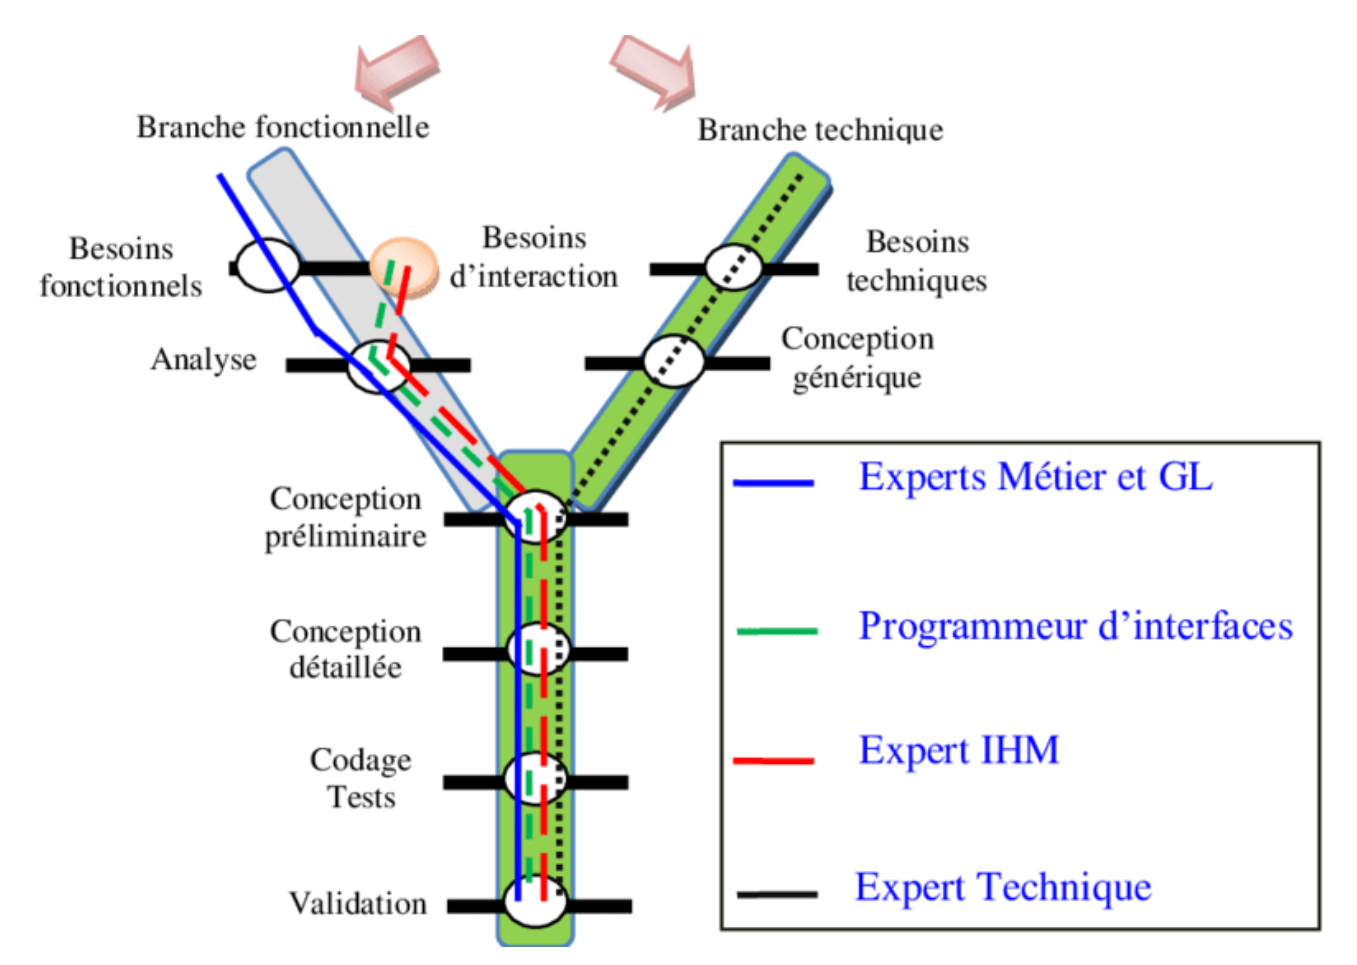
\includegraphics[width=0.75\textwidth]{schema_2tup_Y.png}
	\caption{Structure en Y du processus 2TUP}
	\label{fig:2tup_schema}
\end{figure}

\subsubsection{2TUP et UML}

Le processus 2TUP et le langage UML fonctionnent ensemble : 2TUP utilise UML comme unique langage de modélisation tout au long de ses phases, et chaque livrable produit est un diagramme UML \cite{roques_uml}. Cette cohérence garantit une bonne traçabilité entre les besoins exprimés et les composants réalisés.

Le tableau~\ref{tab:2tup_uml} ci-dessous résume la correspondance entre les phases du 2TUP et les diagrammes UML mobilisés pour «~SALISA~».

\begin{table}[H]
	\centering
	\begin{tabular}{|p{4cm}|p{3.5cm}|p{6cm}|}
		\hline
		\textbf{Phase 2TUP} & \textbf{Branche} & \textbf{Diagrammes UML utilisés} \\
		\hline
		Capture des besoins fonctionnels & Fonctionnelle & Diagramme de contexte statique, Diagramme de cas d'utilisation \\
		\hline
		Spécification détaillée & Fonctionnelle & Diagramme de séquence, Diagramme d'activités \\
		\hline
		Capture des besoins techniques & Technique & Diagramme de déploiement \\
		\hline
		Conception architecturale & Réalisation & Diagramme de composants, Diagramme de déploiement \\
		\hline
		Conception du domaine & Réalisation & Diagramme de classes, Diagramme d'objets \\
		\hline
	\end{tabular}
	\caption{Correspondance entre les phases 2TUP et les diagrammes UML utilisés}
	\label{tab:2tup_uml}
\end{table}

«~SALISA~» combine des besoins fonctionnels nombreux, comme l'inscription des utilisateurs, la mise en correspondance, le paiement ou la messagerie, et des contraintes techniques fortes liées au contexte local, telles que le Mobile Money \cite{mtn_momo}, une connexion parfois limitée ou une architecture distribuée. Le 2TUP permet de traiter ces deux dimensions en parallèle, de façon rigoureuse et coordonnée, ce qui en fait le processus idéal pour notre projet.
	% ============================================================
% PARTIE II - CHAPITRE II : Analyse et Conception
% ============================================================
\chapter{Analyse et Conception}
\pagestyle{styleGlobal}
\label{chap:analyse_conception}

% ============================================================
\section{Analyse du besoin}
% ============================================================

\subsection{Besoins Fonctionnels}

Les besoins fonctionnels représentent l'ensemble des fonctionnalités que «~SALISA~» doit offrir à ses utilisateurs. Nous les avons identifiés à partir de l'analyse des problèmes rencontrés dans la mise en relation manuelle entre prestataires et clients. Ces besoins sont les suivants :

\begin{itemize}
	\item inscription via un numéro de téléphone, avec validation par code OTP ;
	\item connexion et déconnexion sécurisées ;
	\item choix du rôle lors de l'inscription (prestataire, demandeur ou les deux) ;
	\item création et gestion du profil prestataire (informations, portfolio, tarifs, disponibilité, catégories de services) ;
	\item vérification d'identité et obtention de badges de certification ;
	\item publication de missions par le demandeur ;
	\item recherche et filtrage de prestataires par catégorie, arrondissement, disponibilité et budget ;
	\item mise en correspondance intelligente (matching) entre missions et prestataires ;
	\item messagerie directe entre demandeur et prestataire ;
	\item envoi et acceptation de devis structurés ;
	\item paiement sécurisé via Mobile Money (MTN MoMo et Airtel Money) \cite{mtn_momo} ;
	\item sécurisation des fonds par escrow jusqu'à la validation de la mission ;
	\item validation de la mission terminée et libération des fonds ;
	\item gestion des litiges entre prestataires et demandeurs ;
	\item notation et dépôt d'avis après chaque mission réalisée ;
	\item notifications multi-canaux (push PWA, WhatsApp, SMS) ;
	\item tableau de bord de modération pour les administrateurs.
\end{itemize}

\subsection{Besoins Techniques}

Les besoins techniques désignent l'ensemble des contraintes non fonctionnelles auxquelles un système doit se conformer, qu'il s'agisse de performances, de sécurité, de disponibilité ou de compatibilité avec l'environnement d'exécution. Pour «~SALISA~», ces contraintes sont directement liées au contexte congolais, et se déclinent de la façon suivante :

\begin{itemize}
	\item architecture Progressive Web Application (PWA) \cite{next_js}, mobile-first, utilisable depuis tous les terminaux sans installation ;
	\item compatibilité avec les réseaux à faible débit (2G/3G) pour garantir l'accès dans les zones peu couvertes ;
	\item fonctionnement hors ligne partiel pour la consultation des profils et des missions déjà chargés ;
	\item sécurité des échanges par protocoles HTTPS et WSS, authentification par JWT et OTP ;
	\item performance : temps de réponse des API inférieur à 2 secondes pour 95\% des requêtes ;
	\item disponibilité cible de 99,5\% ;
	\item intégration des API de paiement Mobile Money (MTN MoMo et Airtel Money) \cite{mtn_momo} ;
	\item base de données relationnelle (PostgreSQL) \cite{postgresql} avec cache Redis pour les sessions et les résultats fréquents ;
	\item messagerie en temps réel via WebSocket ;
	\item stockage des fichiers (photos de profil, pièces jointes) sur un service cloud externe.
\end{itemize}

% ============================================================
\section{Conception du système}
% ============================================================

\subsection{Spécifications fonctionnelles}

\subsubsection{Identification des acteurs}

Un acteur représente toute entité externe qui interagit avec le système «~SALISA~» \cite{jacobson_up}. Notre système comprend deux catégories d'acteurs : les acteurs humains et les acteurs systèmes.

\vspace{0.3cm}
\noindent\textbf{a- Acteurs humains}

\vspace{0.2cm}
Nous avons identifié quatre principaux acteurs humains :

\begin{itemize}
	\item \textbf{Visiteur :} utilisateur non encore enregistré sur la plateforme. Son unique interaction avec «~SALISA~» est l'inscription, qui lui permet de créer un compte et de devenir un utilisateur à part entière ;
	\item \textbf{Demandeur :} utilisateur connecté qui cherche et embauche des prestataires. Il publie des missions, contacte des prestataires, paie et note les prestations ;
	\item \textbf{Prestataire :} utilisateur connecté qui propose ses services. Il crée son profil, répond aux missions et envoie des devis ;
	\item \textbf{Administrateur :} utilisateur connecté chargé d'administrer la plateforme, de vérifier les identités, de gérer les litiges et de configurer le système.
\end{itemize}

\vspace{0.3cm}
\noindent\textbf{b- Acteurs systèmes}

\vspace{0.2cm}
En modélisation UML, on désigne par acteur système tout composant logiciel extérieur au système étudié qui interagit avec lui par l'échange de données ou de services. Nous en avons identifié deux pour «~SALISA~» :

\begin{itemize}
	\item \textbf{Service de paiement :} regroupe les APIs de MTN MoMo et d'Airtel Money. «~SALISA~» leur envoie des requêtes de paiement et en reçoit des confirmations de transaction \cite{mtn_momo} ;
	\item \textbf{Service de notifications :} regroupe Twilio SMS et WhatsApp Business API. «~SALISA~» lui envoie des instructions pour délivrer les codes OTP, les alertes et les messages aux utilisateurs.
\end{itemize}

\subsubsection{Diagramme de contexte statique}

Le diagramme de contexte statique présente «~SALISA~» au centre et montre toutes les entités externes qui interagissent avec lui. La figure~\ref{fig:contexte_statique} illustre ce diagramme.

\begin{figure}[H]
	\centering
	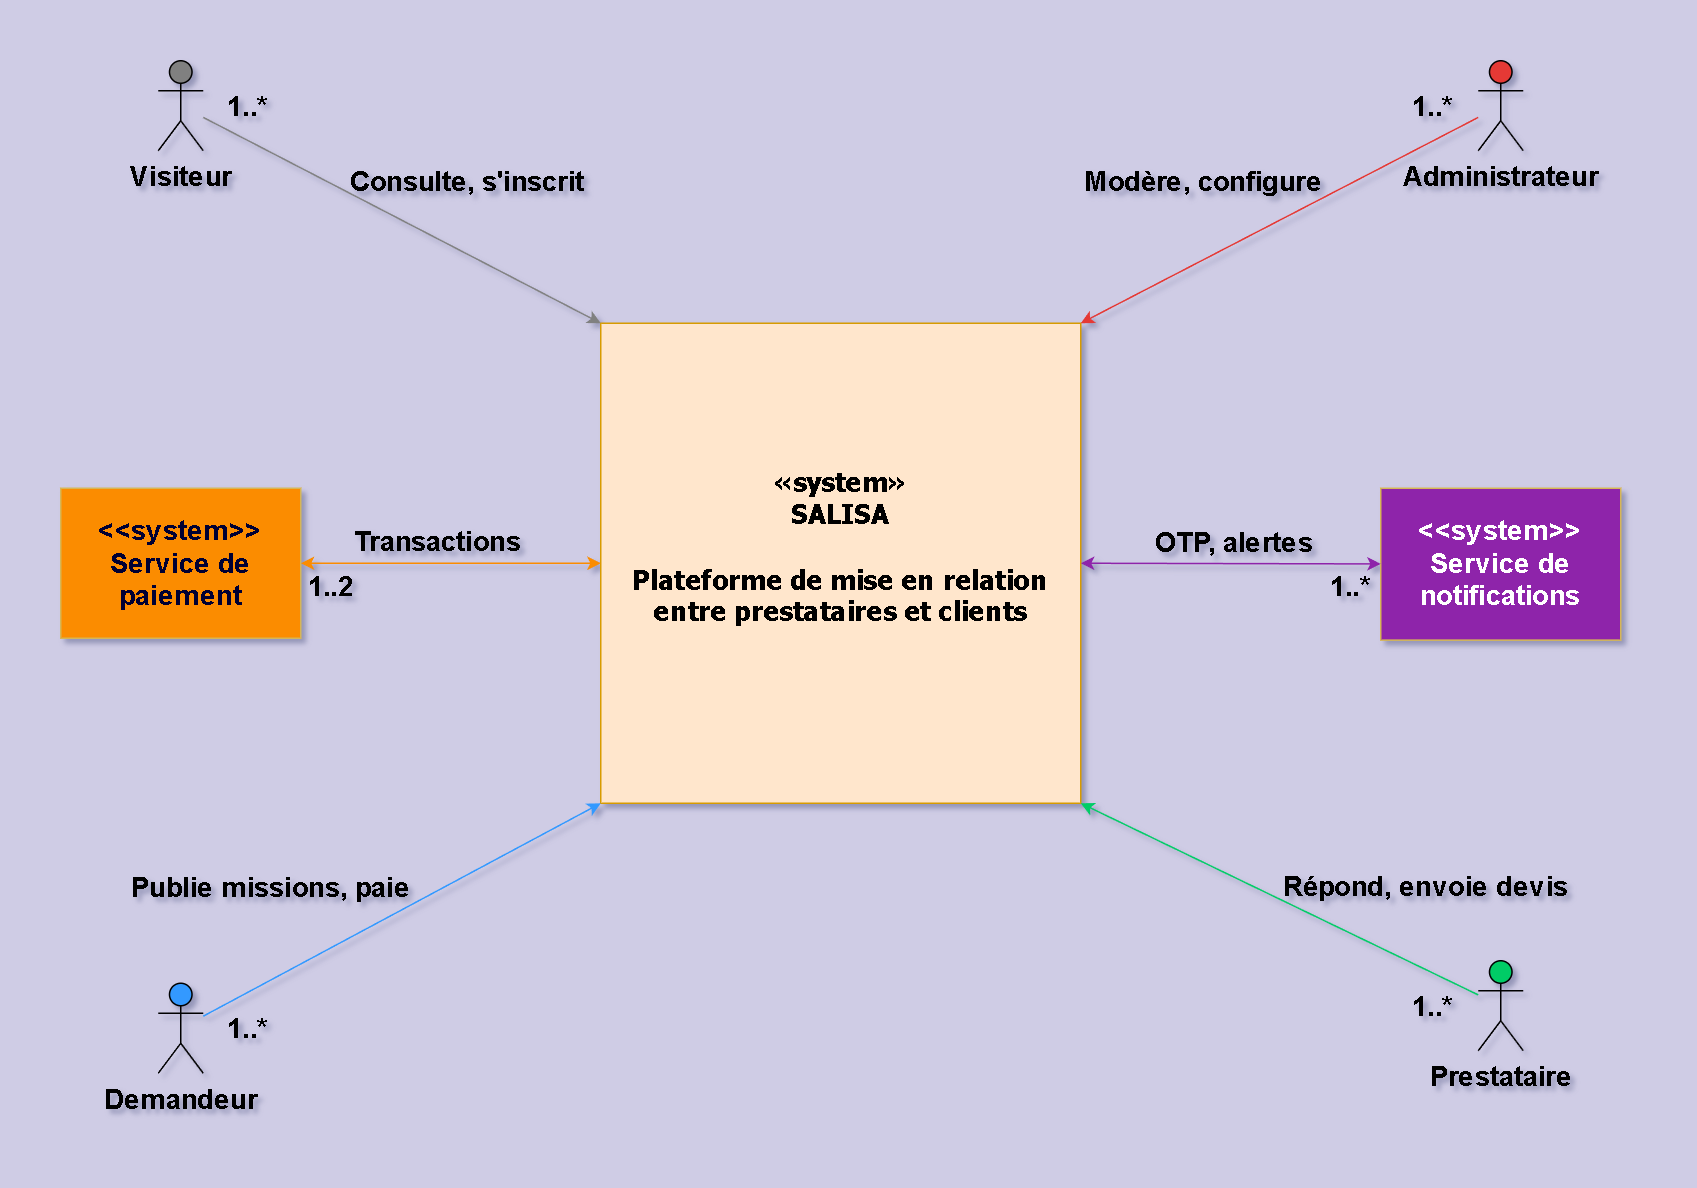
\includegraphics[width=0.95\textwidth]{diagramme_contexte_statique.png}
	\caption{Diagramme de contexte statique de «~SALISA~»}
	\label{fig:contexte_statique}
\end{figure}

Au centre se trouve le système «~SALISA~» représenté par un rectangle. Autour, les quatre acteurs humains (symbole stickman UML) interagissent avec lui : le Visiteur s'inscrit sur la plateforme ; le Demandeur publie des missions, paie et note ; le Prestataire crée son profil, répond et envoie des devis ; l'Administrateur administre et configure. Les deux acteurs systèmes (rectangles avec stéréotype \textit{$\langle\langle$système$\rangle\rangle$}) sont : le service de paiement pour les transactions, et le service de notifications pour les alertes SMS et WhatsApp.

\subsubsection{Identification des cas d'utilisation}

Un cas d'utilisation décrit une interaction entre un acteur et le système pour accomplir un objectif précis. Pour «~SALISA~», nous avons recensé 39 cas d'utilisation, regroupés en neuf familles selon les acteurs concernés. Les tableaux~\ref{tab:cu_f1} à~\ref{tab:cu_f9} présentent le détail de chacune de ces familles.

\begin{table}[H]
	\centering
	\begin{tabular}{|p{3cm}|p{10.5cm}|}
		\hline
		\multicolumn{2}{|c|}{\cellcolor{vertCongo}\textcolor{white}{\textbf{Famille 1 : Authentification et gestion du compte}}} \\
		\hline
		\rowcolor{vertCongo}
		\textcolor{white}{\textbf{Cas d'utilisation}} & \textcolor{white}{\textbf{Définition}} \\
		\hline
		\textbf{UC-01} & s'inscrire via numéro de téléphone (Visiteur) \\
		\hline
		\textbf{UC-02} & valider le code OTP (Visiteur) \\
		\hline
		\textbf{UC-03} & choisir son rôle lors de l'inscription (Visiteur) \\
		\hline
		\textbf{UC-04} & se connecter (Demandeur, Prestataire, Administrateur) \\
		\hline
		\textbf{UC-05} & se déconnecter (Demandeur, Prestataire, Administrateur) \\
		\hline
	\end{tabular}
	\caption{Cas d'utilisation de la famille F1 : Authentification et gestion du compte}
	\label{tab:cu_f1}
\end{table}

\begin{table}[H]
	\centering
	\begin{tabular}{|p{3cm}|p{10.5cm}|}
		\hline
		\multicolumn{2}{|c|}{\cellcolor{vertCongo}\textcolor{white}{\textbf{Famille 2 : Gestion du profil prestataire}}} \\
		\hline
		\rowcolor{vertCongo}
		\textcolor{white}{\textbf{Cas d'utilisation}} & \textcolor{white}{\textbf{Définition}} \\
		\hline
		\textbf{UC-06} & compléter son profil prestataire (Prestataire) \\
		\hline
		\textbf{UC-07} & gérer son portfolio (Prestataire) \\
		\hline
		\textbf{UC-08} & définir ses tarifs et sa disponibilité (Prestataire) \\
		\hline
		\textbf{UC-09} & gérer ses catégories et compétences (Prestataire) \\
		\hline
		\textbf{UC-10} & faire vérifier son identité pour obtenir le badge Vérifié (Prestataire, Administrateur) \\
		\hline
	\end{tabular}
	\caption{Cas d'utilisation de la famille F2 : Gestion du profil prestataire}
	\label{tab:cu_f2}
\end{table}

\begin{table}[H]
	\centering
	\begin{tabular}{|p{3cm}|p{10.5cm}|}
		\hline
		\multicolumn{2}{|c|}{\cellcolor{vertCongo}\textcolor{white}{\textbf{Famille 3 : Gestion des missions}}} \\
		\hline
		\rowcolor{vertCongo}
		\textcolor{white}{\textbf{Cas d'utilisation}} & \textcolor{white}{\textbf{Définition}} \\
		\hline
		\textbf{UC-11} & publier une mission (Demandeur) \\
		\hline
		\textbf{UC-12} & utiliser l'assistant IA pour la description (Demandeur) \\
		\hline
		\textbf{UC-13} & gérer ses missions publiées (Demandeur) \\
		\hline
	\end{tabular}
	\caption{Cas d'utilisation de la famille F3 : Gestion des missions}
	\label{tab:cu_f3}
\end{table}

\begin{table}[H]
	\centering
	\begin{tabular}{|p{3cm}|p{10.5cm}|}
		\hline
		\multicolumn{2}{|c|}{\cellcolor{vertCongo}\textcolor{white}{\textbf{Famille 4 : Recherche et matching}}} \\
		\hline
		\rowcolor{vertCongo}
		\textcolor{white}{\textbf{Cas d'utilisation}} & \textcolor{white}{\textbf{Définition}} \\
		\hline
		\textbf{UC-14} & rechercher un prestataire (Demandeur) \\
		\hline
		\textbf{UC-15} & filtrer les résultats de recherche (Demandeur) \\
		\hline
		\textbf{UC-16} & consulter le score de matching (Demandeur) \\
		\hline
		\textbf{UC-17} & recevoir des suggestions proactives de prestataires (Demandeur) \\
		\hline
		\textbf{UC-18} & consulter le profil d'un prestataire (Demandeur) \\
		\hline
	\end{tabular}
	\caption{Cas d'utilisation de la famille F4 : Recherche et matching}
	\label{tab:cu_f4}
\end{table}

\begin{table}[H]
	\centering
	\begin{tabular}{|p{3cm}|p{10.5cm}|}
		\hline
		\multicolumn{2}{|c|}{\cellcolor{vertCongo}\textcolor{white}{\textbf{Famille 5 : Messagerie et devis}}} \\
		\hline
		\rowcolor{vertCongo}
		\textcolor{white}{\textbf{Cas d'utilisation}} & \textcolor{white}{\textbf{Définition}} \\
		\hline
		\textbf{UC-19} & envoyer un message (Demandeur, Prestataire) \\
		\hline
		\textbf{UC-20} & envoyer un devis (Prestataire) \\
		\hline
		\textbf{UC-21} & accepter un devis (Demandeur) \\
		\hline
		\textbf{UC-22} & refuser ou demander une modification de devis (Demandeur) \\
		\hline
	\end{tabular}
	\caption{Cas d'utilisation de la famille F5 : Messagerie et devis}
	\label{tab:cu_f5}
\end{table}

\begin{table}[H]
	\centering
	\begin{tabular}{|p{3cm}|p{10.5cm}|}
		\hline
		\multicolumn{2}{|c|}{\cellcolor{vertCongo}\textcolor{white}{\textbf{Famille 6 : Paiement et escrow}}} \\
		\hline
		\rowcolor{vertCongo}
		\textcolor{white}{\textbf{Cas d'utilisation}} & \textcolor{white}{\textbf{Définition}} \\
		\hline
		\textbf{UC-23} & payer une mission via Mobile Money (Demandeur, service de paiement) \\
		\hline
		\textbf{UC-24} & choisir MTN MoMo comme moyen de paiement (Demandeur) \\
		\hline
		\textbf{UC-25} & choisir Airtel Money comme moyen de paiement (Demandeur) \\
		\hline
		\textbf{UC-26} & valider la mission terminée (Demandeur) \\
		\hline
		\textbf{UC-27} & scanner le code QR de validation sur place (Prestataire) \\
		\hline
		\textbf{UC-28} & ouvrir un litige (Demandeur, Prestataire) \\
		\hline
		\textbf{UC-29} & demander un retrait Mobile Money (Prestataire) \\
		\hline
	\end{tabular}
	\caption{Cas d'utilisation de la famille F6 : Paiement et escrow}
	\label{tab:cu_f6}
\end{table}

\begin{table}[H]
	\centering
	\begin{tabular}{|p{3cm}|p{10.5cm}|}
		\hline
		\multicolumn{2}{|c|}{\cellcolor{vertCongo}\textcolor{white}{\textbf{Famille 7 : Notation et réputation}}} \\
		\hline
		\rowcolor{vertCongo}
		\textcolor{white}{\textbf{Cas d'utilisation}} & \textcolor{white}{\textbf{Définition}} \\
		\hline
		\textbf{UC-30} & laisser un avis après mission (Demandeur, Prestataire) \\
		\hline
		\textbf{UC-31} & signaler un avis abusif (Demandeur, Prestataire) \\
		\hline
	\end{tabular}
	\caption{Cas d'utilisation de la famille F7 : Notation et réputation}
	\label{tab:cu_f7}
\end{table}

\begin{table}[H]
	\centering
	\begin{tabular}{|p{3cm}|p{10.5cm}|}
		\hline
		\multicolumn{2}{|c|}{\cellcolor{vertCongo}\textcolor{white}{\textbf{Famille 8 : Notifications}}} \\
		\hline
		\rowcolor{vertCongo}
		\textcolor{white}{\textbf{Cas d'utilisation}} & \textcolor{white}{\textbf{Définition}} \\
		\hline
		\textbf{UC-32} & recevoir des notifications multi-canaux (Demandeur, Prestataire, service de notifications) \\
		\hline
		\textbf{UC-33} & configurer ses préférences de notification (Demandeur, Prestataire) \\
		\hline
	\end{tabular}
	\caption{Cas d'utilisation de la famille F8 : Notifications}
	\label{tab:cu_f8}
\end{table}

\begin{table}[H]
	\centering
	\begin{tabular}{|p{3cm}|p{10.5cm}|}
		\hline
		\multicolumn{2}{|c|}{\cellcolor{vertCongo}\textcolor{white}{\textbf{Famille 9 : Administration}}} \\
		\hline
		\rowcolor{vertCongo}
		\textcolor{white}{\textbf{Cas d'utilisation}} & \textcolor{white}{\textbf{Définition}} \\
		\hline
		\textbf{UC-34} & accéder au tableau de bord de modération (Administrateur) \\
		\hline
		\textbf{UC-35} & valider ou rejeter une vérification d'identité (Administrateur) \\
		\hline
		\textbf{UC-36} & gérer les signalements (Administrateur) \\
		\hline
		\textbf{UC-37} & suspendre un compte utilisateur (Administrateur) \\
		\hline
		\textbf{UC-38} & configurer le système (Administrateur) \\
		\hline
		\textbf{UC-39} & consulter les statistiques avancées (Administrateur) \\
		\hline
	\end{tabular}
	\caption{Cas d'utilisation de la famille F9 : Administration}
	\label{tab:cu_f9}
\end{table}

\subsubsection{Relation entre les cas d'utilisation}

Les relations entre cas d'utilisation permettent de structurer et de clarifier les dépendances entre les fonctionnalités du système \cite{roques_uml}. On en distingue deux types principaux. La relation \textbf{$\langle\langle$include$\rangle\rangle$} indique qu'un cas d'utilisation est toujours exécuté dans le cadre d'un autre : par exemple, UC-01 (s'inscrire) inclut systématiquement UC-02 (valider le code OTP), car on ne peut pas créer de compte sans valider le code reçu par SMS ; de même, UC-21 (accepter un devis) inclut UC-23 (payer via Mobile Money), car l'acceptation d'un devis déclenche toujours le processus de paiement. La relation \textbf{$\langle\langle$extend$\rangle\rangle$}, quant à elle, indique qu'un cas d'utilisation est exécuté de façon optionnelle dans certaines conditions : par exemple, UC-11 (publier une mission) peut optionnellement étendre vers UC-12 (utiliser l'assistant IA), selon le choix du demandeur, et UC-26 (valider la mission) peut étendre vers UC-27 (scanner le code QR), uniquement pour les missions réalisées en présentiel.

\vspace{0.4cm}
La figure~\ref{fig:cu_global} présente le diagramme de cas d'utilisation global de «~SALISA~», organisé autour des neuf familles fonctionnelles.

\begin{figure}[H]
	\centering
	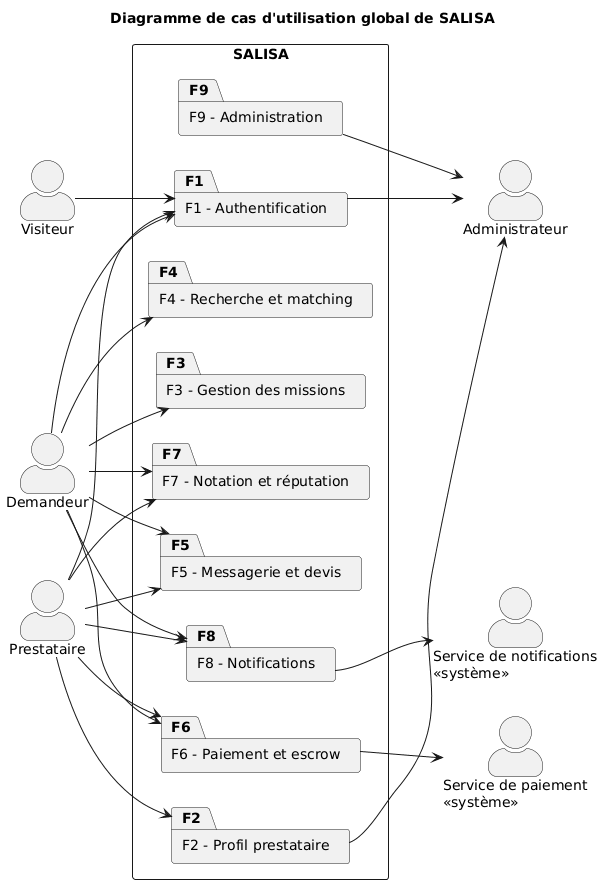
\includegraphics[width=0.95\textwidth]{diagramme_cu_global.png}
	\caption{Diagramme de cas d'utilisation global de «~SALISA~»}
	\label{fig:cu_global}
\end{figure}

Pour une meilleure lisibilité, chaque famille est ensuite détaillée dans un diagramme dédié, présentant les cas d'utilisation et leurs relations avec précision. Les figures~\ref{fig:cu_f1} à~\ref{fig:cu_f9} illustrent ces neuf diagrammes.

\begin{figure}[H]
	\centering
	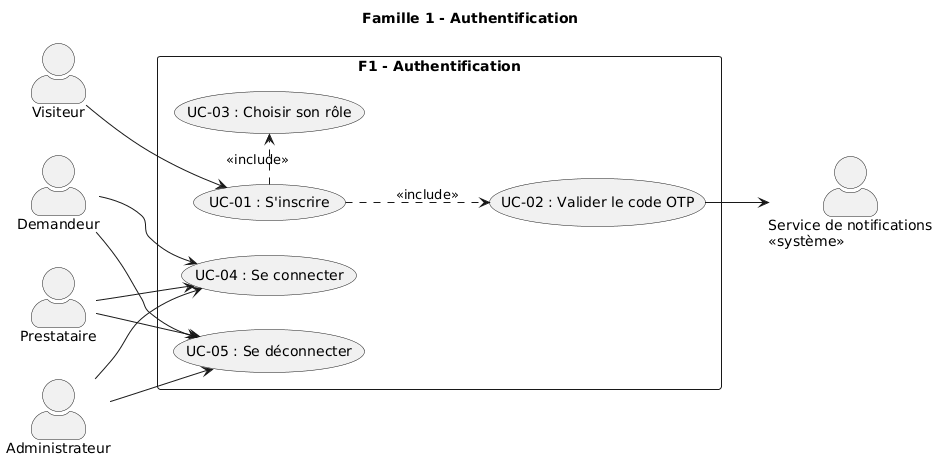
\includegraphics[width=0.85\textwidth]{diagramme_cu_f1.png}
	\caption{Diagramme de cas d'utilisation - F1 : Authentification}
	\label{fig:cu_f1}
\end{figure}

\begin{figure}[H]
	\centering
	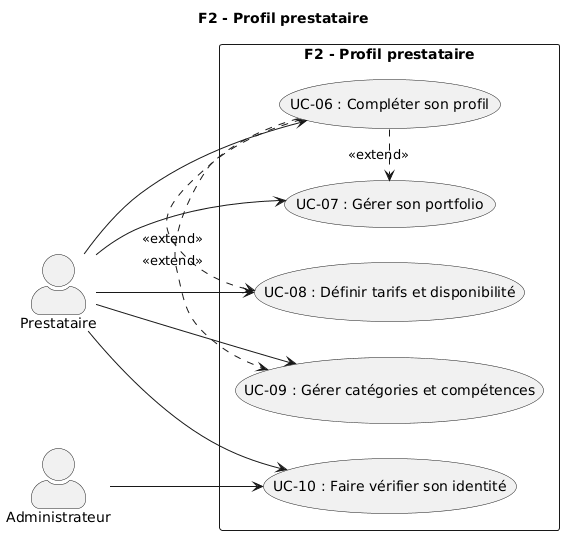
\includegraphics[width=0.85\textwidth]{diagramme_cu_f2.png}
	\caption{Diagramme de cas d'utilisation - F2 : Profil prestataire}
	\label{fig:cu_f2}
\end{figure}

\begin{figure}[H]
	\centering
	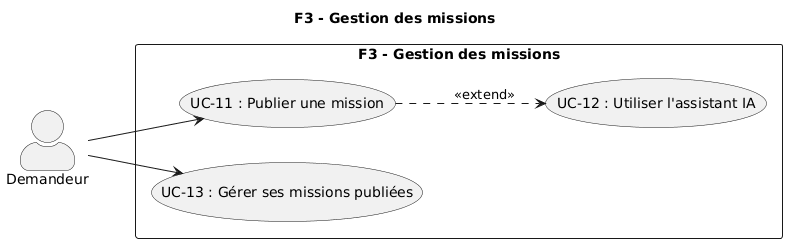
\includegraphics[width=0.85\textwidth]{diagramme_cu_f3.png}
	\caption{Diagramme de cas d'utilisation - F3 : Gestion des missions}
	\label{fig:cu_f3}
\end{figure}

\begin{figure}[H]
	\centering
	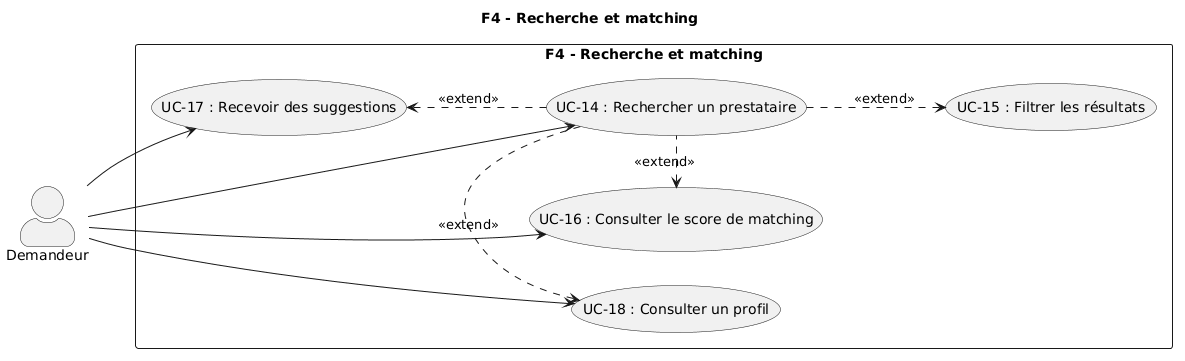
\includegraphics[width=0.85\textwidth]{diagramme_cu_f4.png}
	\caption{Diagramme de cas d'utilisation - F4 : Recherche et matching}
	\label{fig:cu_f4}
\end{figure}

\begin{figure}[H]
	\centering
	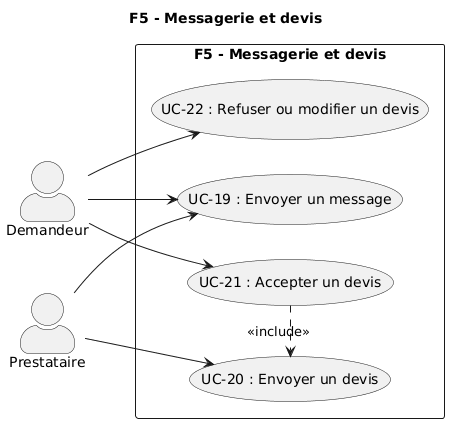
\includegraphics[width=0.85\textwidth]{diagramme_cu_f5.png}
	\caption{Diagramme de cas d'utilisation - F5 : Messagerie et devis}
	\label{fig:cu_f5}
\end{figure}

\begin{figure}[H]
	\centering
	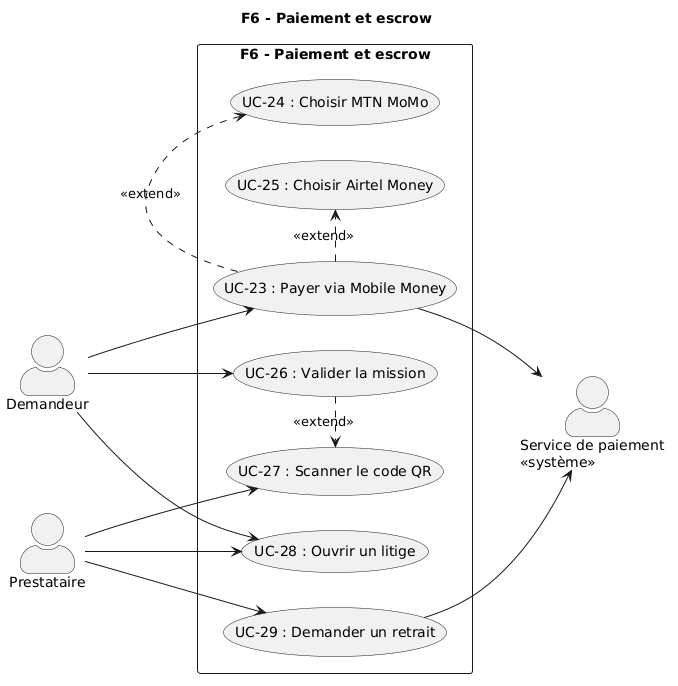
\includegraphics[width=0.85\textwidth]{diagramme_cu_f6.png}
	\caption{Diagramme de cas d'utilisation - F6 : Paiement et escrow}
	\label{fig:cu_f6}
\end{figure}

\begin{figure}[H]
	\centering
	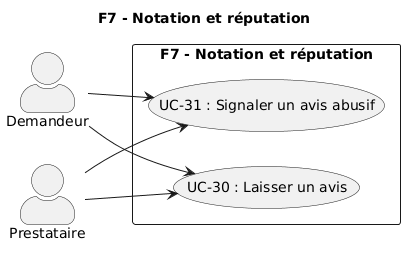
\includegraphics[width=0.85\textwidth]{diagramme_cu_f7.png}
	\caption{Diagramme de cas d'utilisation - F7 : Notation et réputation}
	\label{fig:cu_f7}
\end{figure}

\begin{figure}[H]
	\centering
	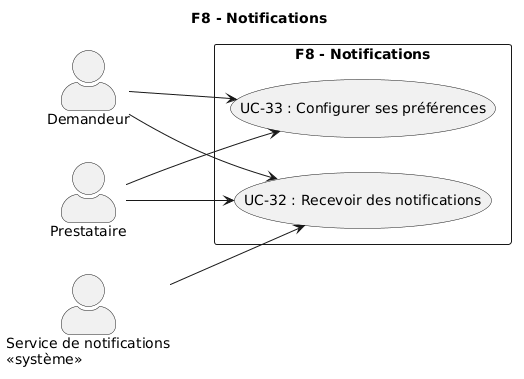
\includegraphics[width=0.85\textwidth]{diagramme_cu_f8.png}
	\caption{Diagramme de cas d'utilisation - F8 : Notifications}
	\label{fig:cu_f8}
\end{figure}

\begin{figure}[H]
	\centering
	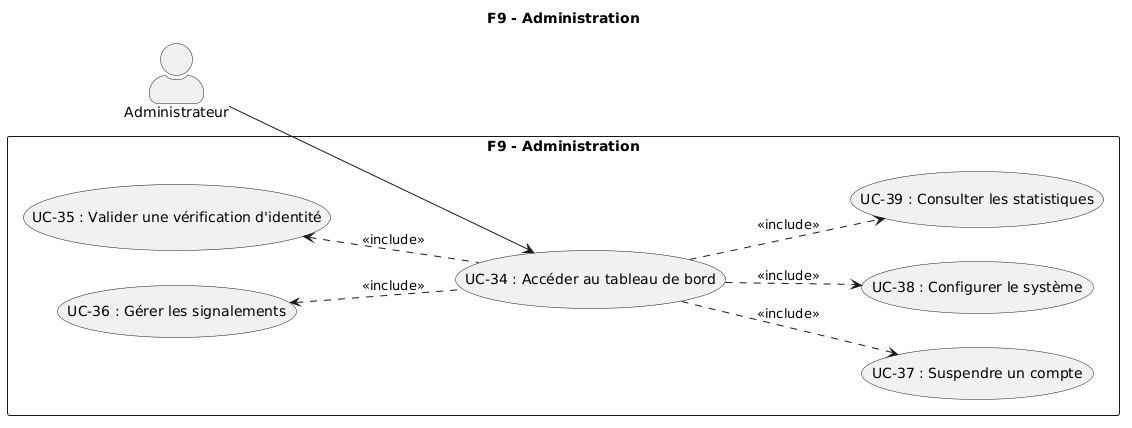
\includegraphics[width=0.85\textwidth]{diagramme_cu_f9.png}
	\caption{Diagramme de cas d'utilisation - F9 : Administration}
	\label{fig:cu_f9}
\end{figure}

\subsubsection{Classification des cas d'utilisation (priorités, risques et itérations)}

Le tableau~\ref{tab:classification_cu} présente la classification des principaux cas d'utilisation selon leur priorité fonctionnelle, leur niveau de risque technique et l'itération de développement dans laquelle ils s'inscrivent. L'itération 1 regroupe les fonctionnalités essentielles au fonctionnement minimal du système. L'itération 2 contient les fonctionnalités importantes mais non bloquantes. L'itération 3 rassemble les fonctionnalités souhaitables à plus long terme.

\begin{table}[H]
	\centering
	\begin{tabular}{|c|p{4.5cm}|c|c|c|}
		\hline
		\rowcolor{vertCongo}
		\textcolor{white}{\textbf{UC}} &
		\textcolor{white}{\textbf{Libellé}} &
		\textcolor{white}{\textbf{Priorité}} &
		\textcolor{white}{\textbf{Risque}} &
		\textcolor{white}{\textbf{Itération}} \\
		\hline
		UC-01 & s'inscrire & Élevée & Élevé & 1 \\
		\hline
		UC-02 & valider le code OTP & Élevée & Élevé & 1 \\
		\hline
		UC-03 & choisir son rôle & Élevée & Faible & 1 \\
		\hline
		UC-06 & compléter son profil & Élevée & Moyen & 1 \\
		\hline
		UC-11 & publier une mission & Élevée & Moyen & 1 \\
		\hline
		UC-14 & rechercher un prestataire & Élevée & Moyen & 1 \\
		\hline
		UC-19 & envoyer un message & Élevée & Moyen & 1 \\
		\hline
		UC-20 & envoyer un devis & Élevée & Moyen & 1 \\
		\hline
		UC-23 & payer via Mobile Money & Élevée & Élevé & 1 \\
		\hline
		UC-26 & valider la mission & Élevée & Élevé & 1 \\
		\hline
		UC-30 & laisser un avis & Élevée & Faible & 1 \\
		\hline
		UC-32 & recevoir des notifications & Élevée & Moyen & 1 \\
		\hline
		UC-34 & tableau de bord admin & Élevée & Moyen & 1 \\
		\hline
		UC-12 & utiliser l'assistant IA & Moyenne & Élevé & 2 \\
		\hline
		UC-16 & score de matching & Moyenne & Élevé & 2 \\
		\hline
		UC-28 & ouvrir un litige & Moyenne & Moyen & 2 \\
		\hline
		UC-38 & configurer le système & Basse & Faible & 3 \\
		\hline
	\end{tabular}
	\caption{Classification des principaux cas d'utilisation de «~SALISA~»}
	\label{tab:classification_cu}
\end{table}

\subsection{Spécification détaillée}

\subsubsection{Description textuelle des cas d'utilisation (au plus 2 cu)}

\noindent\textbf{a- Description de UC-01 : s'inscrire via numéro de téléphone}

\vspace{0.2cm}
\begin{table}[H]
	\centering
	\begin{tabular}{|p{3.5cm}|p{10cm}|}
		\hline
		\rowcolor{vertClair}
		\textbf{Cas d'utilisation} & UC-01 : s'inscrire via numéro de téléphone \\
		\hline
		\textbf{Acteur principal} & Visiteur \\
		\hline
		\textbf{Précondition} & le visiteur n'a pas encore de compte sur «~SALISA~» \\
		\hline
		\textbf{Déclencheur} & le visiteur clique sur le bouton «~S'inscrire~» \\
		\hline
		\textbf{Scénario nominal} &
		\begin{enumerate}
			\item Le visiteur saisit son numéro de téléphone au format +242 XXXXXXXXX.
			\item Le système valide le format et envoie un code OTP par SMS (UC-02).
			\item Le visiteur saisit le code OTP reçu.
			\item Le système vérifie le code (durée de validité : 5 minutes).
			\item Le visiteur choisit son rôle : prestataire, demandeur, ou les deux (UC-03).
			\item Le compte est créé et le visiteur devient un utilisateur connecté.
		\end{enumerate} \\
		\hline
		\textbf{Scénarios alternatifs} &
		\begin{itemize}
			\item Code OTP expiré : le visiteur peut en demander un nouveau.
			\item 3 tentatives échouées : blocage temporaire de 10 minutes.
			\item Numéro déjà existant : redirection vers la page de connexion.
		\end{itemize} \\
		\hline
		\textbf{Postcondition} & le compte est créé ; le visiteur est devenu un utilisateur et peut accéder à toutes les fonctionnalités selon son rôle \\
		\hline
	\end{tabular}
	\caption{Description textuelle de UC-01 : s'inscrire via numéro de téléphone}
	\label{tab:uc01}
\end{table}

\vspace{0.5cm}
\noindent\textbf{b- Description de UC-11 : publier une mission}

\vspace{0.2cm}
\begin{table}[H]
	\centering
	\begin{tabular}{|p{3.5cm}|p{10cm}|}
		\hline
		\rowcolor{vertClair}
		\textbf{Cas d'utilisation} & UC-11 : publier une mission \\
		\hline
		\textbf{Acteur principal} & Demandeur \\
		\hline
		\textbf{Précondition} & l'utilisateur est connecté en tant que demandeur \\
		\hline
		\textbf{Déclencheur} & le demandeur clique sur «~Publier une mission~» \\
		\hline
		\textbf{Scénario nominal} &
		\begin{enumerate}
			\item Le demandeur saisit le titre de la mission.
			\item Il renseigne la description de son besoin (ou utilise l'assistant IA - UC-12).
			\item Il sélectionne la catégorie et l'arrondissement.
			\item Il indique le budget et le délai souhaité.
			\item Il confirme et publie la mission.
			\item Le système lance l'algorithme de matching et notifie les prestataires correspondants.
		\end{enumerate} \\
		\hline
		\textbf{Scénarios alternatifs} &
		\begin{itemize}
			\item Le demandeur n'est pas connecté : redirection vers la page de connexion.
			\item Aucun prestataire ne correspond : message «~Aucun résultat proche~».
		\end{itemize} \\
		\hline
		\textbf{Postcondition} & la mission est publiée et les prestataires correspondants sont notifiés \\
		\hline
	\end{tabular}
	\caption{Description textuelle de UC-11 : publier une mission}
	\label{tab:uc11}
\end{table}

\subsubsection{Diagramme de séquence (au plus 2)}

La figure~\ref{fig:seq_inscription} illustre le diagramme de séquence du cas d'utilisation UC-01 (s'inscrire via numéro de téléphone).

\begin{figure}[H]
	\centering
	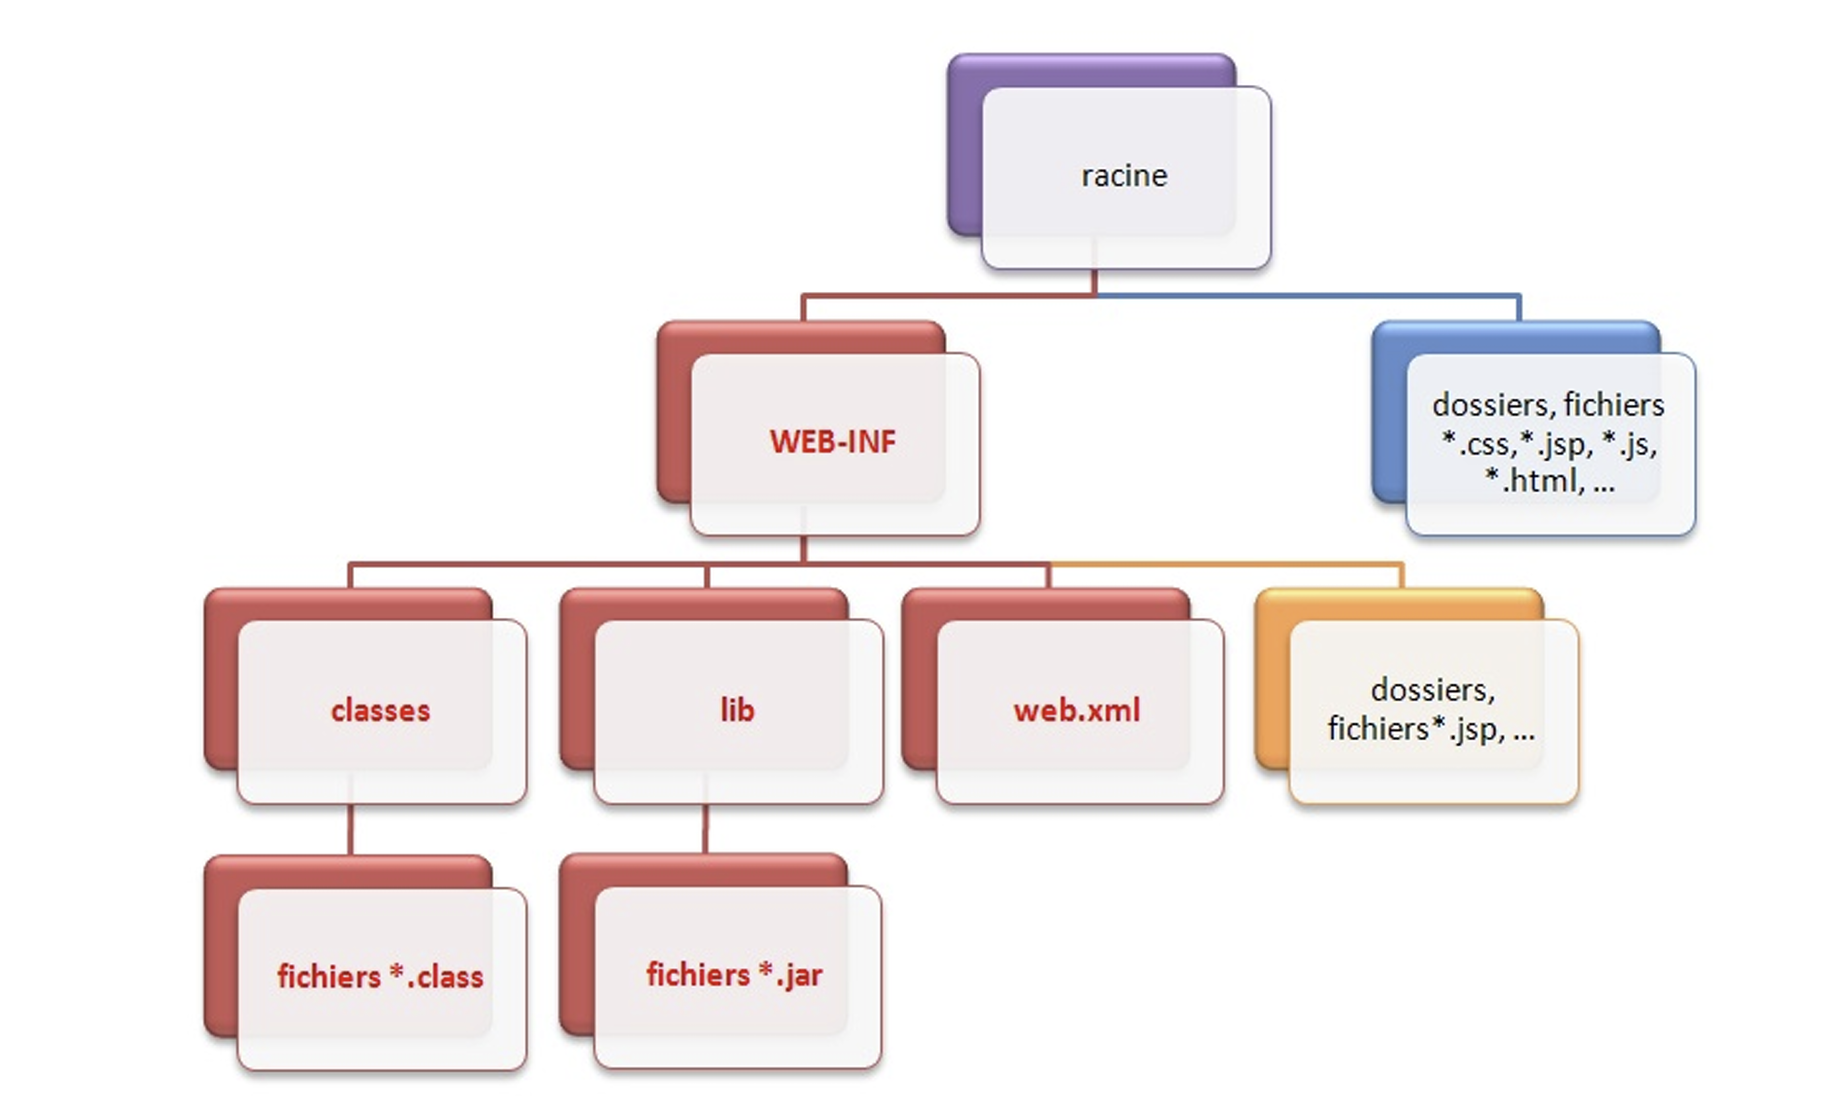
\includegraphics[width=0.95\textwidth]{diagramme_sequence_inscription.png}
	\caption{Diagramme de séquence - inscription via numéro de téléphone (UC-01)}
	\label{fig:seq_inscription}
\end{figure}

La figure~\ref{fig:seq_paiement} illustre le diagramme de séquence du scénario de paiement et de libération des fonds (UC-23 et UC-26).

\begin{figure}[H]
	\centering
	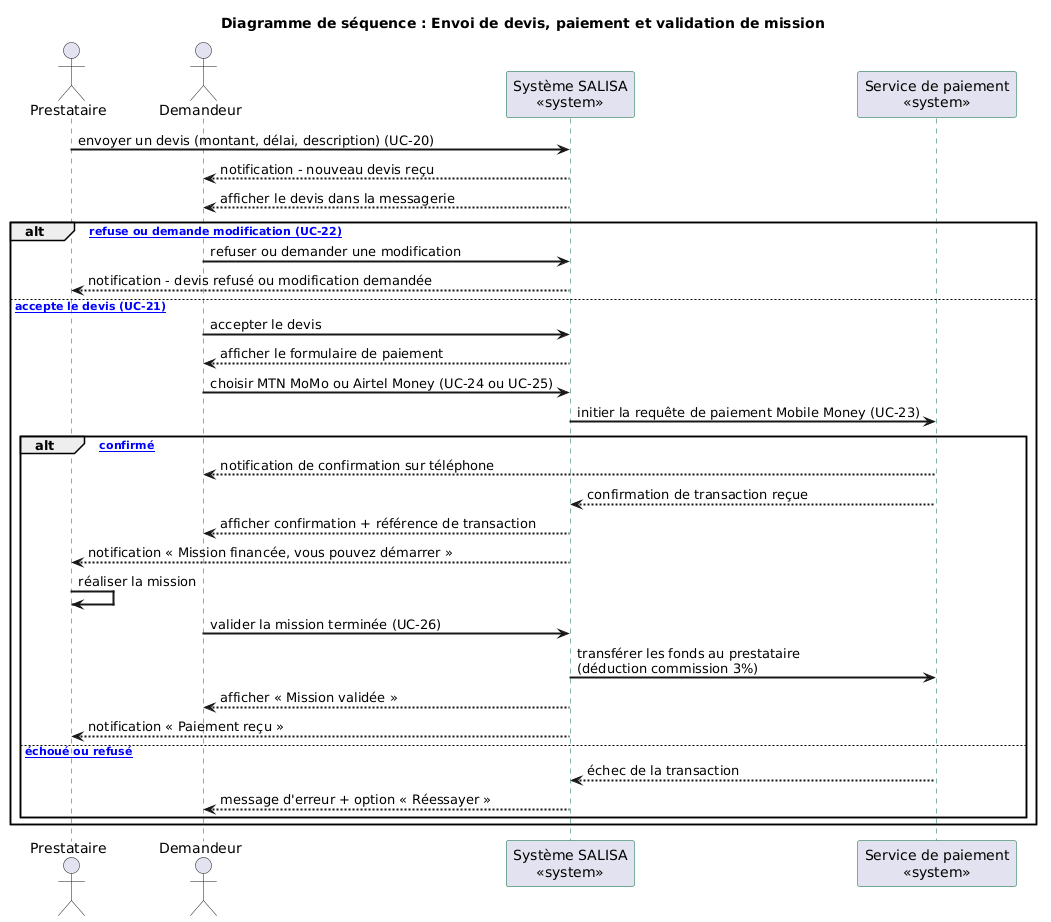
\includegraphics[width=0.95\textwidth]{diagramme_sequence_paiement.png}
	\caption{Diagramme de séquence - paiement et libération des fonds (UC-23 et UC-26)}
	\label{fig:seq_paiement}
\end{figure}

\subsubsection{Diagramme d'activités (au plus 2)}

La figure~\ref{fig:act_publication} présente le diagramme d'activités du processus de publication d'une mission.

\begin{figure}[H]
	\centering
	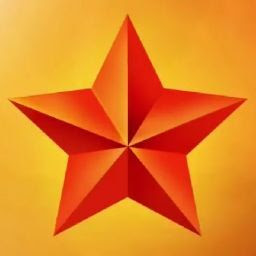
\includegraphics[width=0.95\textwidth]{diagramme_activites_mission.png}
	\caption{Diagramme d'activités - publication de mission et sélection du prestataire}
	\label{fig:act_publication}
\end{figure}

La figure~\ref{fig:act_paiement} illustre le diagramme d'activités du processus de paiement sécurisé par escrow.

\begin{figure}[H]
	\centering
	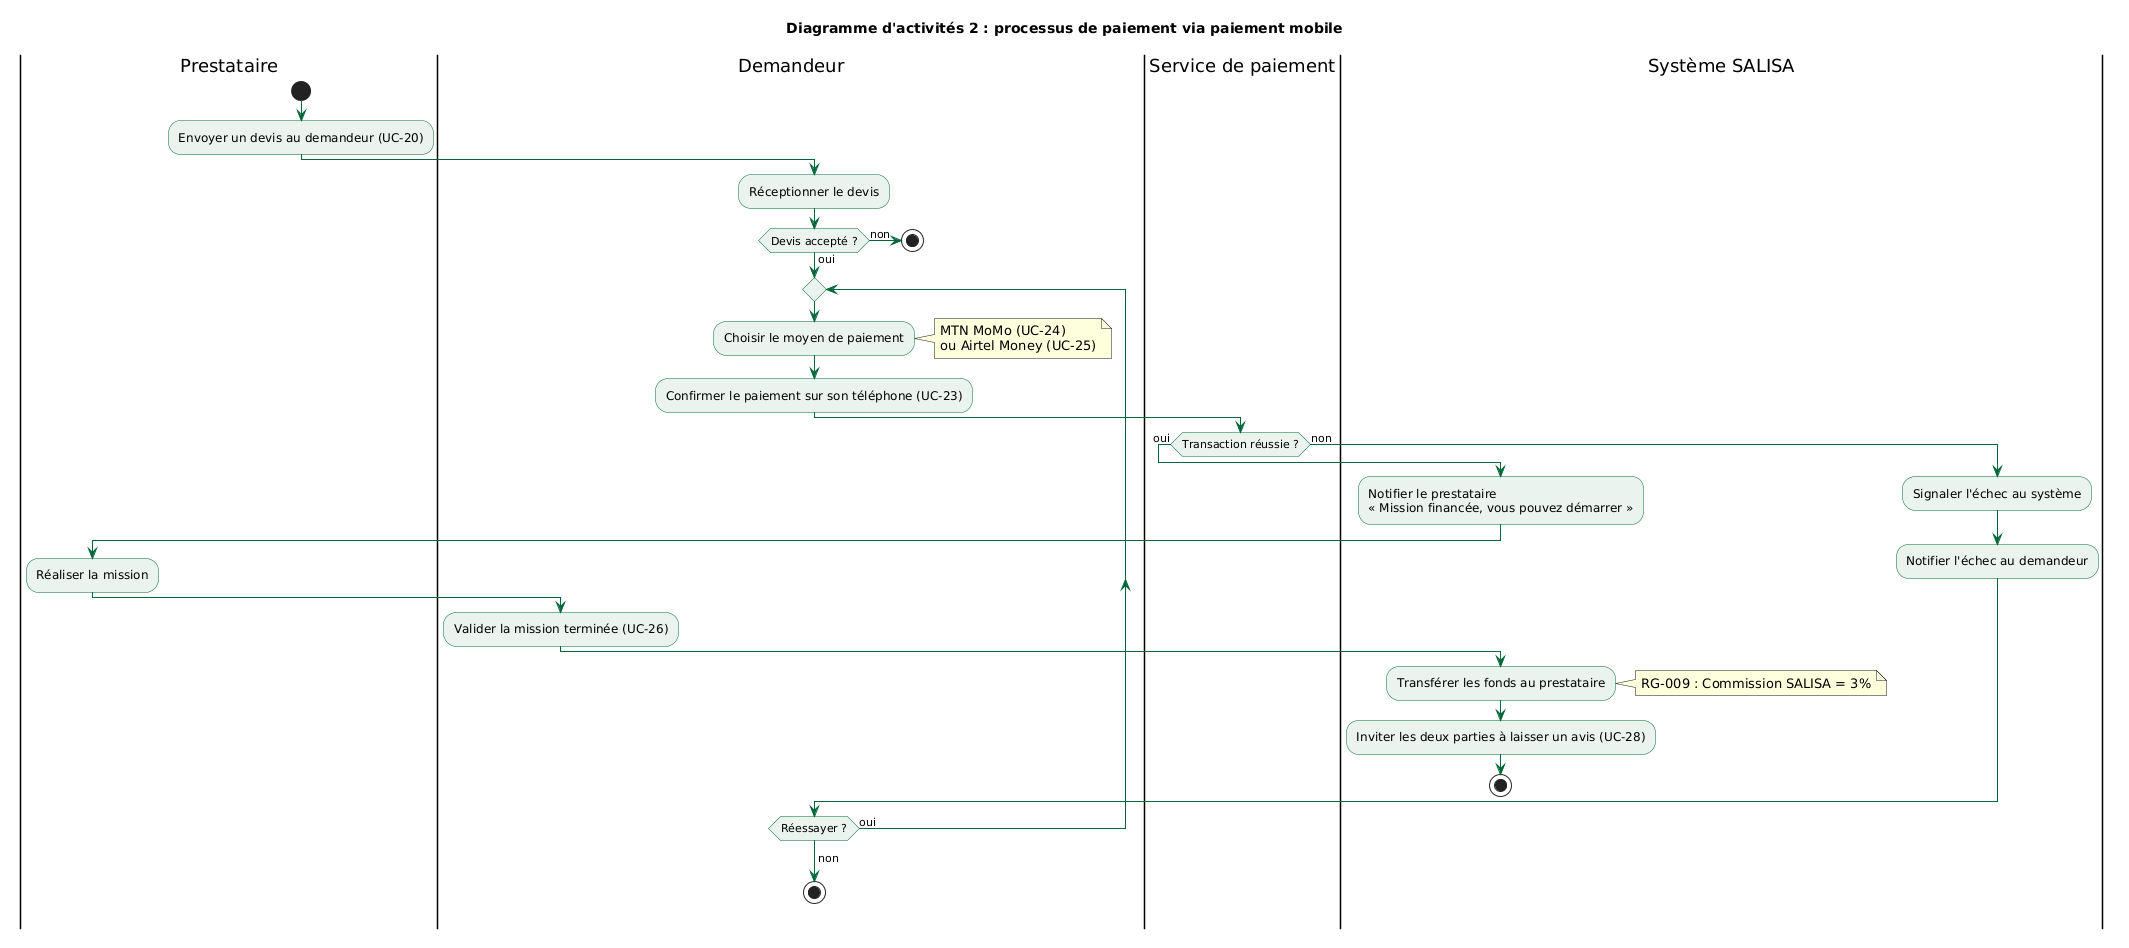
\includegraphics[width=0.95\textwidth]{diagramme_activites_paiement.png}
	\caption{Diagramme d'activités - paiement sécurisé par escrow}
	\label{fig:act_paiement}
\end{figure}

\subsection{Réalisation des cas d'utilisation}

\subsubsection{Quelques règles de gestion}

Les règles de gestion définissent le comportement du système «~SALISA~» dans des situations précises \cite{roques_uml}. Elles garantissent la cohérence des données et la fiabilité des transactions.

\vspace{0.2cm}
\noindent\textbf{Gestion des comptes}

\begin{itemize}
	\item RG-001 : un numéro de téléphone ne peut être associé qu'à un seul compte ;
	\item RG-002 : un même compte peut avoir simultanément les rôles de prestataire et de demandeur ;
	\item RG-003 : un compte est suspendu automatiquement après trois signalements validés par un administrateur ;
	\item RG-004 : lors de la suppression d'un compte, les données sont conservées 30 jours avant effacement définitif.
\end{itemize}

\noindent\textbf{Gestion des missions et des prestataires}

\begin{itemize}
	\item RG-010 : un profil prestataire n'est visible dans la recherche qu'à partir de 70\% de complétion ;
	\item RG-011 : un prestataire avec un compte gratuit ne peut postuler qu'à 3 missions par mois ;
	\item RG-012 : une mission sans activité depuis 30 jours est archivée automatiquement ;
	\item RG-013 : au maximum 10 prestataires sont notifiés par mission (les 10 meilleurs scores de matching).
\end{itemize}

\noindent\textbf{Gestion des paiements}

\begin{itemize}
	\item RG-020 : la commission de «~SALISA~» est de 8\% du montant total de chaque transaction ;
	\item RG-021 : le montant minimum d'une transaction est de 2 000 FCFA ;
	\item RG-022 : si le demandeur ne valide pas la mission dans les 7 jours suivant la livraison, les fonds sont libérés automatiquement au prestataire ;
	\item RG-023 : un litige doit être ouvert dans les 48 heures suivant la date de livraison prévue.
\end{itemize}

\noindent\textbf{Gestion des avis}

\begin{itemize}
	\item RG-030 : un avis ne peut être laissé qu'après une mission avec transaction validée ;
	\item RG-031 : le délai pour laisser un avis est de 14 jours après la validation de la mission ;
	\item RG-032 : les avis sont définitifs et ne peuvent jamais être supprimés par le prestataire ou le demandeur.
\end{itemize}

\subsubsection{Modèle du domaine (Diagramme de classe du système)}

La figure~\ref{fig:diag_classes} présente le diagramme de classes de «~SALISA~», qui représente les entités principales du système, leurs attributs, leurs méthodes et les relations qui les unissent \cite{booch_uml}.

\begin{figure}[H]
	\centering
	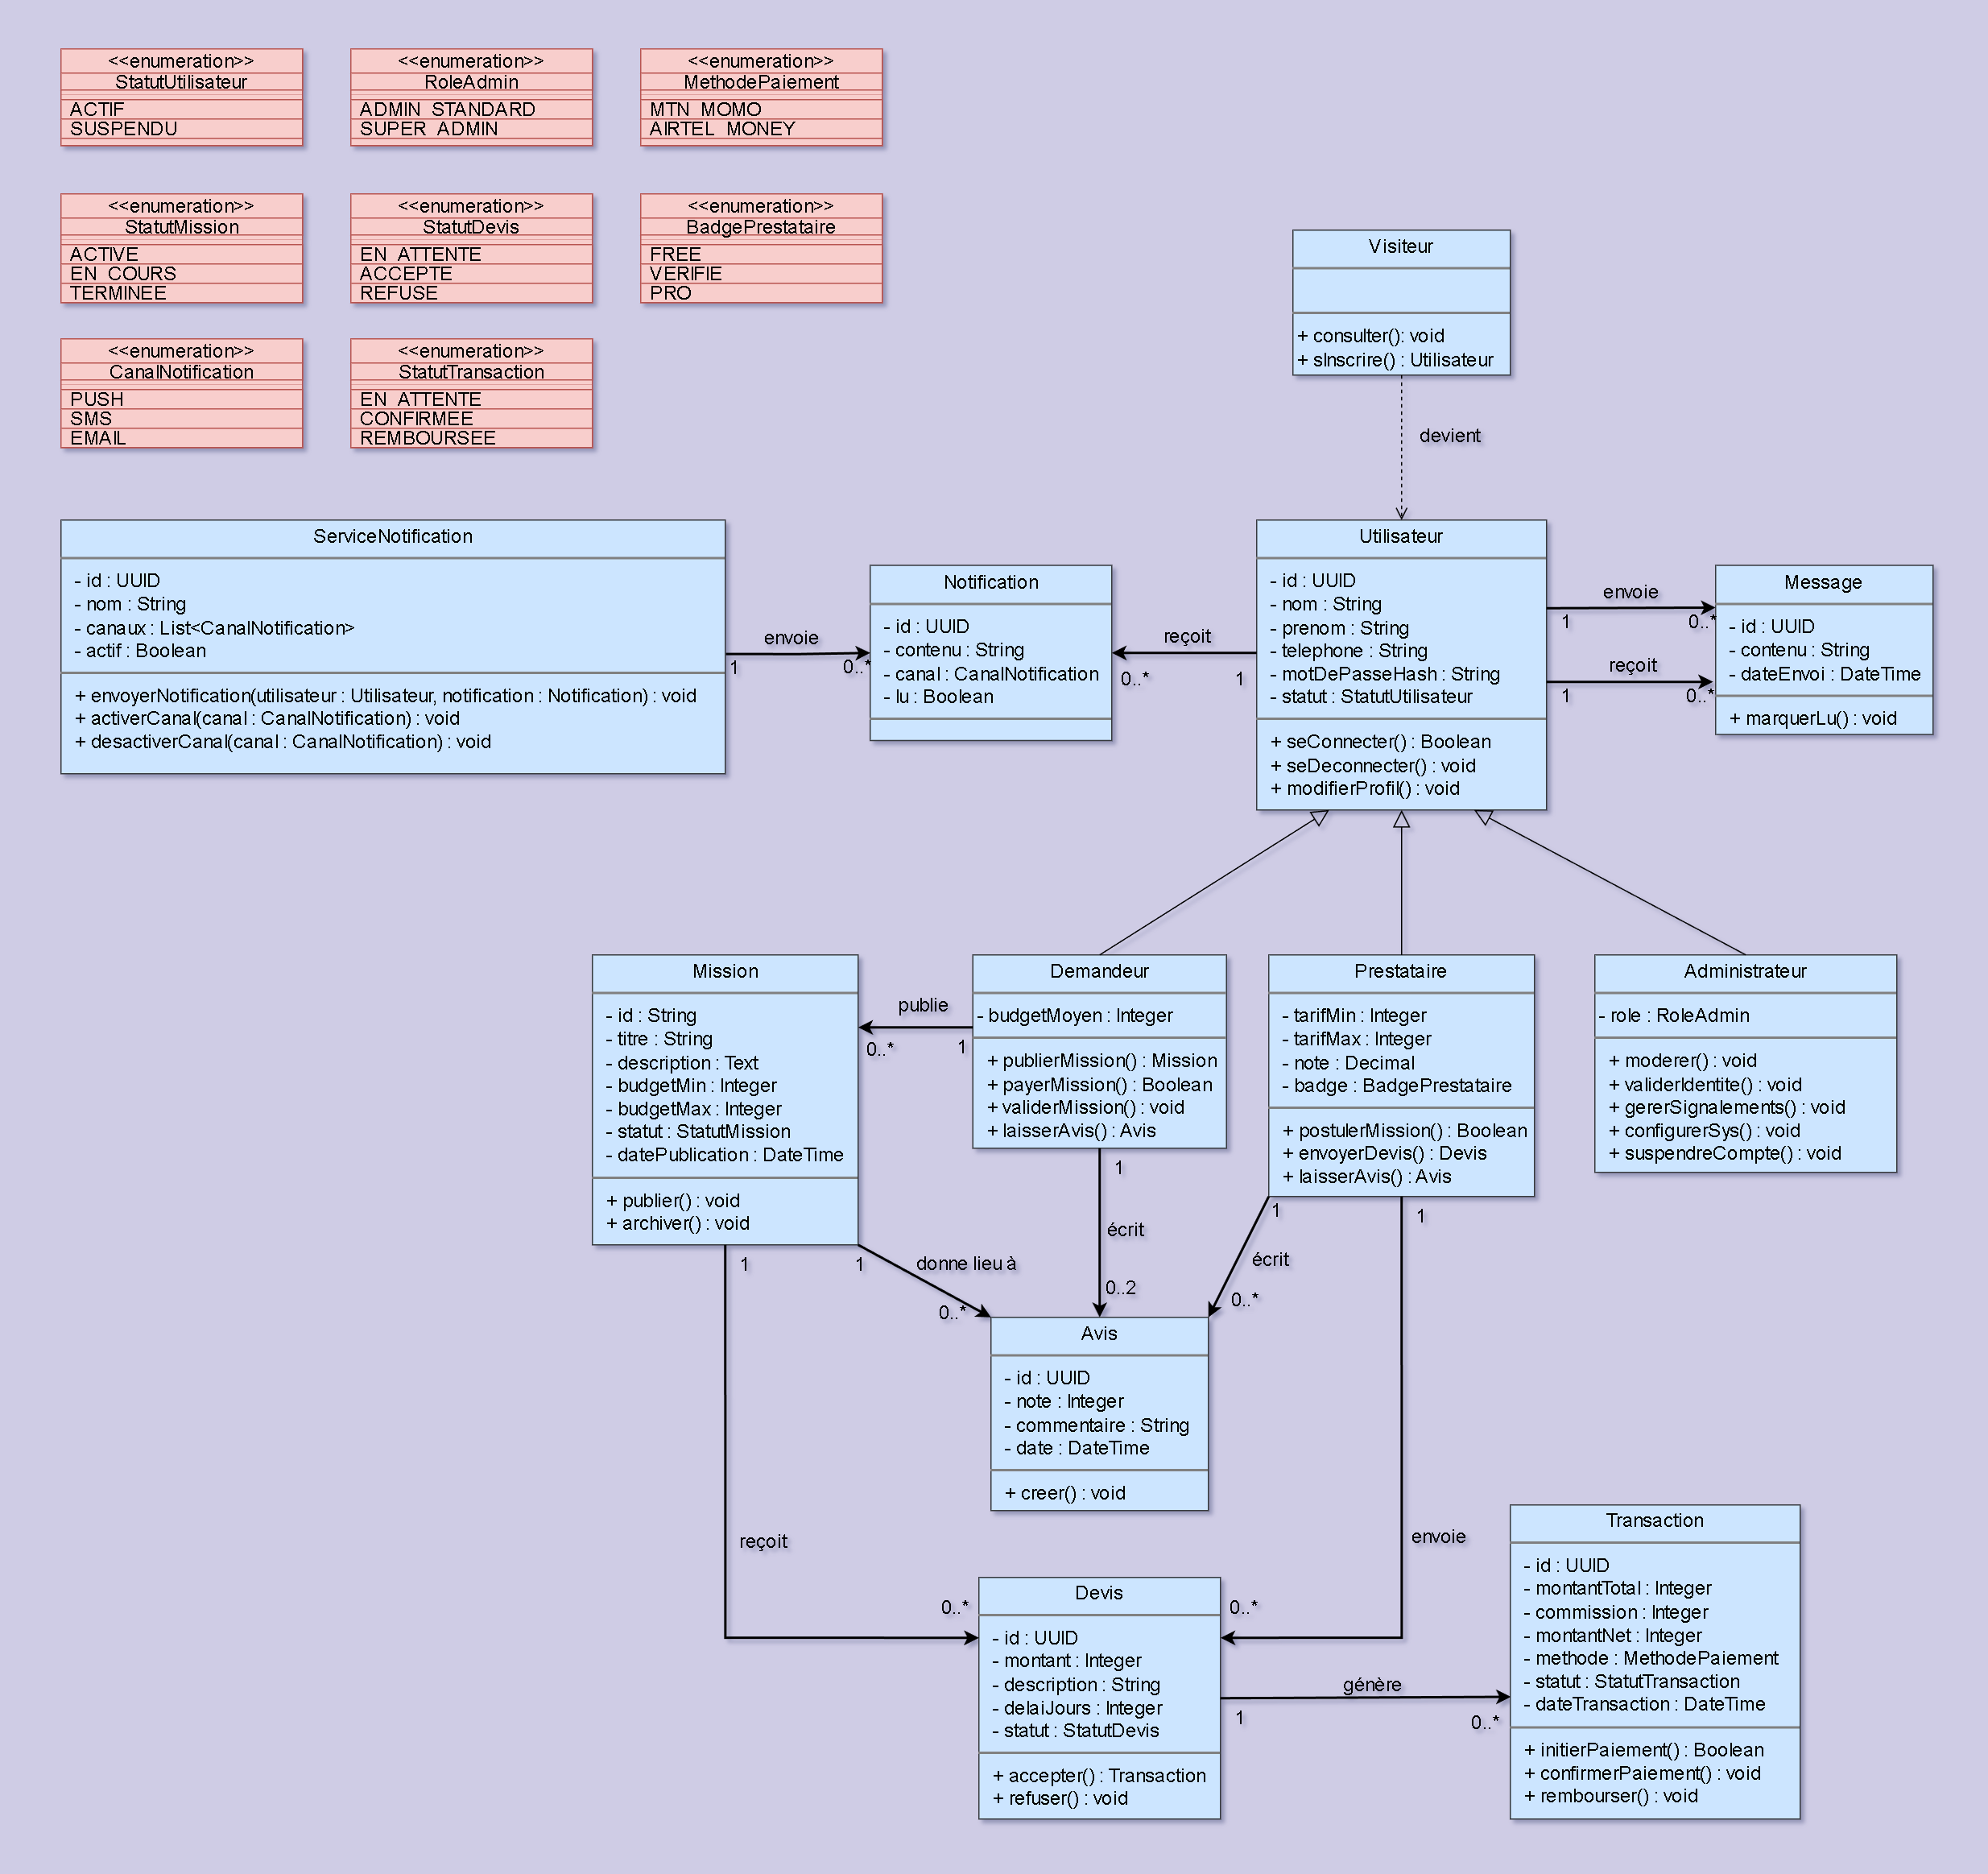
\includegraphics[width=0.95\textwidth]{diagramme_classes.png}
	\caption{Diagramme de classes du système «~SALISA~»}
	\label{fig:diag_classes}
\end{figure}

\subsubsection{Diagramme d'Objets}

La figure~\ref{fig:diag_objets} illustre un exemple d'instanciation du système «~SALISA~», correspondant au scénario où un demandeur publie une mission, un prestataire y répond avec un devis, et le paiement est sécurisé par escrow.

\begin{figure}[H]
	\centering
	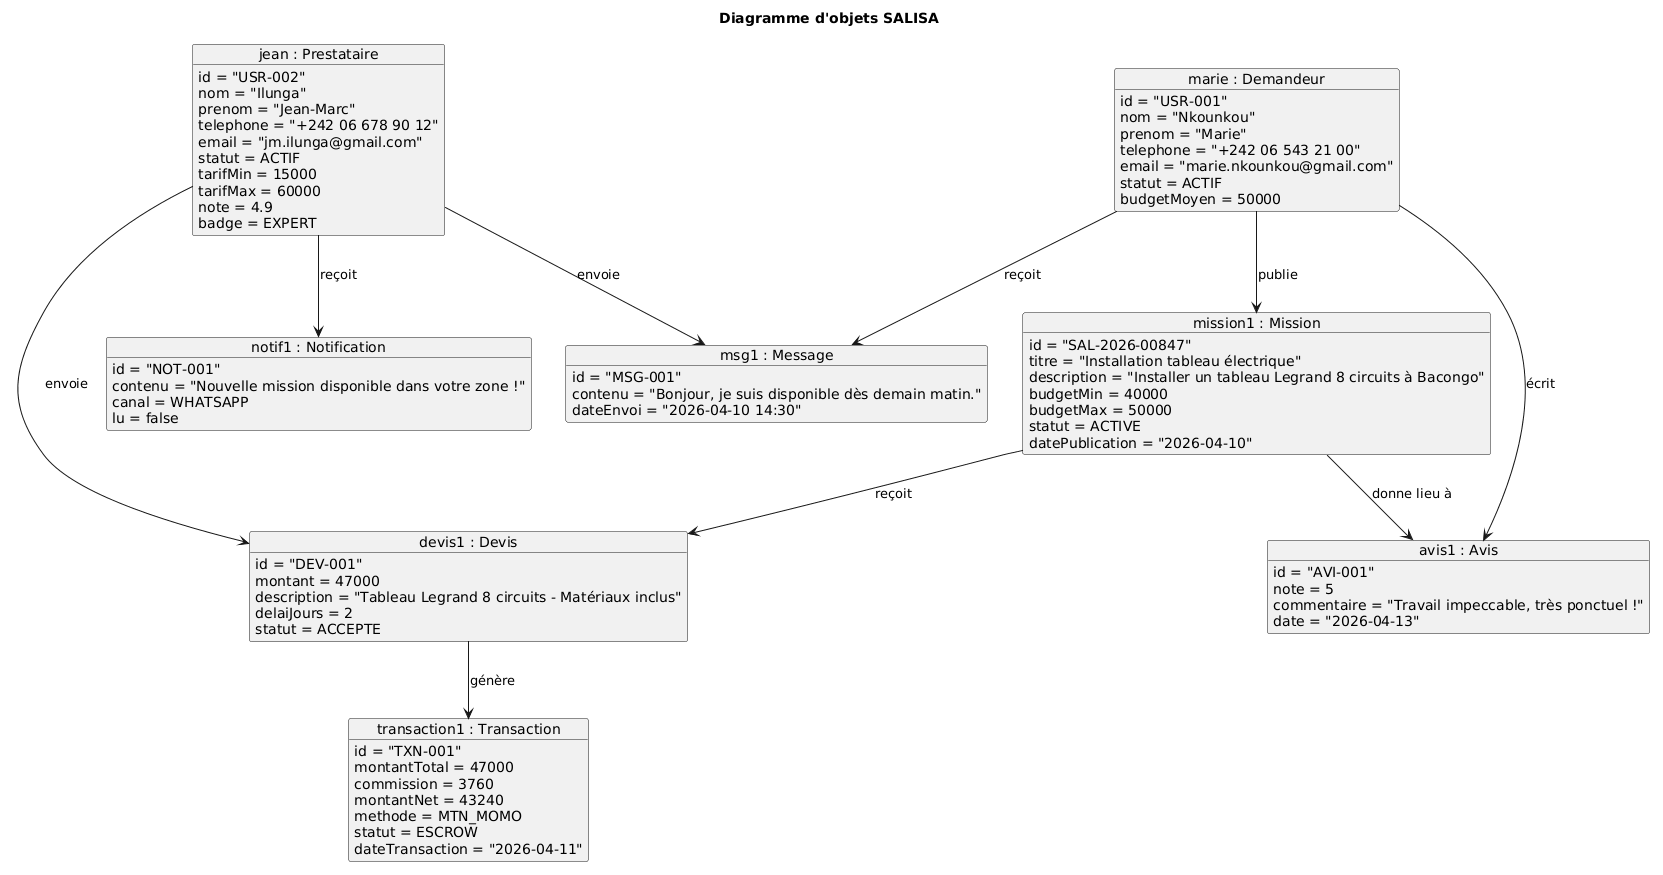
\includegraphics[width=0.95\textwidth]{diagramme_objets.png}
	\caption{Diagramme d'objets - scénario de publication et réponse à une mission}
	\label{fig:diag_objets}
\end{figure}

\subsection{Conception architecturale}

\subsubsection{Architecture logicielle}

«~SALISA~» repose sur une architecture modulaire organisée autour de cinq couches principales.

Le \textbf{front-end} est développé en Next.js 14 \cite{next_js}, un framework React qui permet de générer des pages côté serveur (SSR) et des pages statiques (SSG). Il assure l'aspect PWA mobile-first et l'optimisation pour les réseaux lents.

Le \textbf{back-end} est développé en Node.js avec Express.js. Il expose une API REST pour toutes les opérations classiques et utilise Socket.io pour la messagerie en temps réel via WebSocket.

La \textbf{base de données} principale est PostgreSQL \cite{postgresql}, qui stocke toutes les données persistantes (utilisateurs, missions, transactions, avis). Redis est utilisé comme cache pour les sessions et les résultats de recherche fréquents.

Le \textbf{service de matching} est un microservice Python développé avec FastAPI. Il calcule les scores de compatibilité entre les missions et les prestataires sur la base de huit critères pondérés : localisation, disponibilité, compétences, budget, note, fiabilité, temps de réponse et niveau de badge.

Le \textbf{service de notifications} est un worker asynchrone qui envoie les alertes via trois canaux : les notifications push PWA, les messages WhatsApp et les SMS.

\subsubsection{Architecture globale de la solution (Diagramme de déploiement)}

La figure~\ref{fig:diag_deploiement} présente le diagramme de déploiement de «~SALISA~», qui montre la répartition des composants sur les équipements matériels et les services en ligne.

\begin{figure}[H]
	\centering
	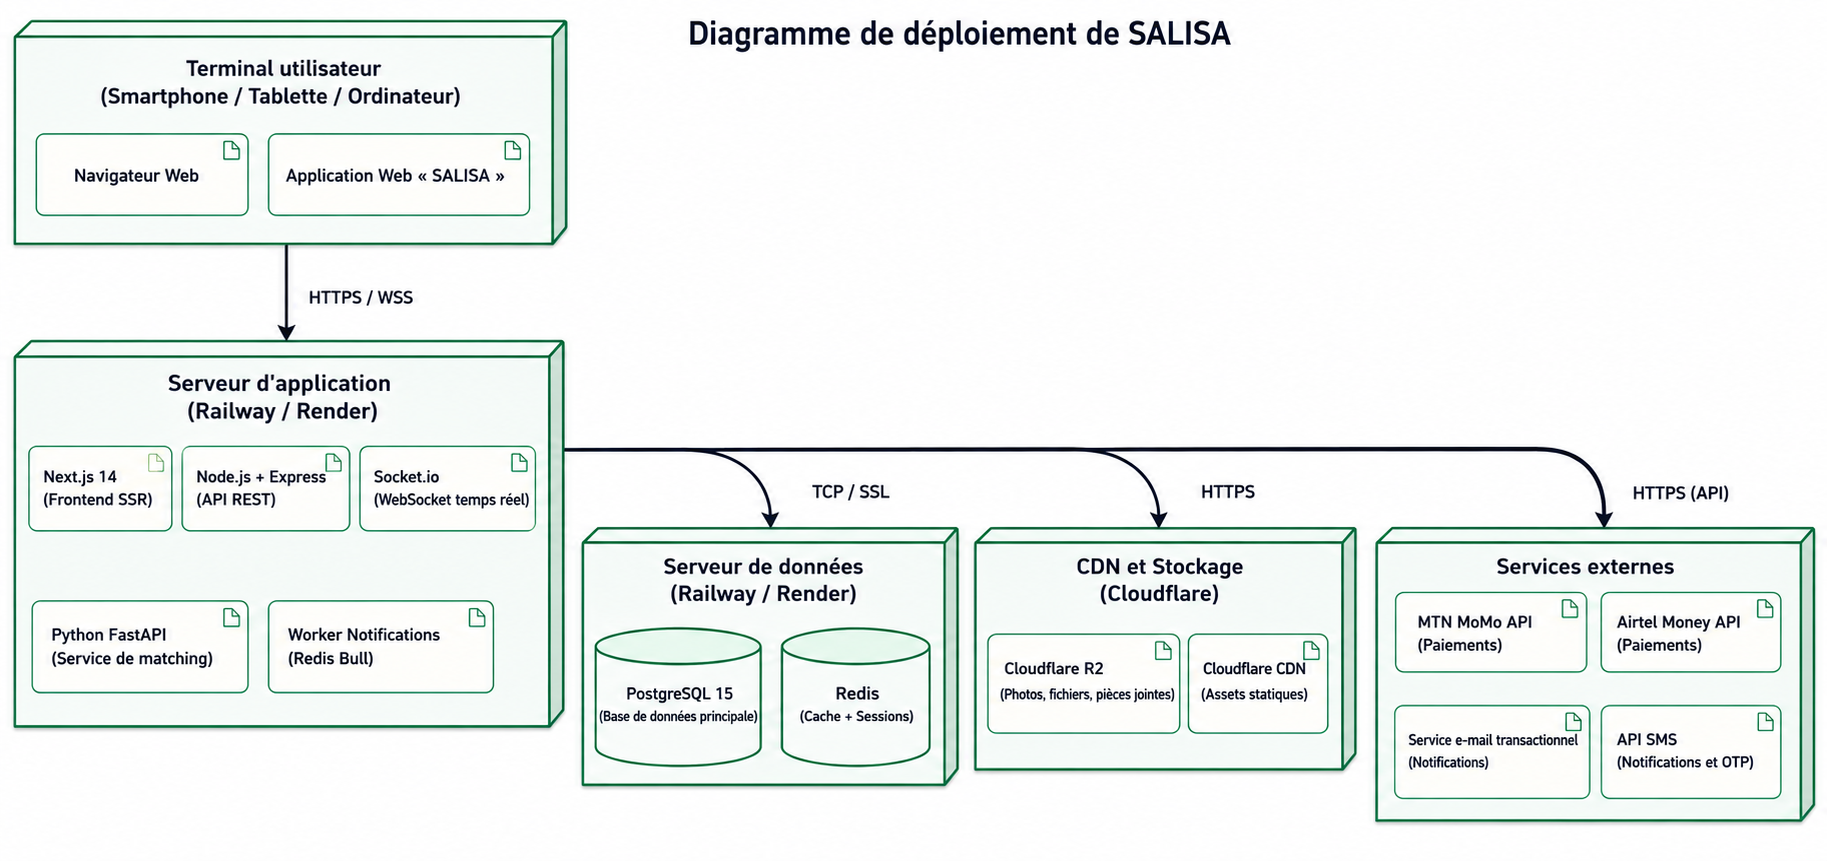
\includegraphics[width=0.95\textwidth]{diagramme_deploiement.png}
	\caption{Diagramme de déploiement de «~SALISA~»}
	\label{fig:diag_deploiement}
\end{figure}
	
	% ---- TROISIEME PARTIE ----
	\pagePartieAnnonce%
	{Troisième Partie}%
	{ÉVALUATION ET RÉALISATION DU PROJET}%
	{Troisième Partie : Évaluation et Réalisation du Projet}
	\setcounter{chapter}{0}
	
	% ============================================================
% PARTIE III - CHAPITRE I : L'évaluation du projet
% ============================================================
\chapter{L'évaluation du projet}
\pagestyle{styleGlobal}
\label{chap:evaluation}

% ============================================================
\section{Organisation du projet}
% ============================================================

« SALISA » a été réalisé dans le cadre de l'obtention du diplôme de Licence Professionnelle
en Génie Logiciel à l'École Supérieure de Gestion et d'Administration des Entreprises (ESGAE)
de Brazzaville. Il s'agit d'un projet de fin d'études mené en binôme, sous la supervision d'un
Directeur de Projet (DP).

La conduite du projet repose sur des séances de travail hebdomadaires avec le Directeur de
Projet, tenues chaque samedi. Ces séances permettent de faire le point sur l'avancement, de
valider les livrables et d'orienter les prochaines étapes. La méthode de développement adoptée
est le \textbf{2TUP}, combinée au langage de modélisation \textbf{UML}.

% ============================================================
\section{Intervenants}
% ============================================================

Plusieurs acteurs ont participé à la réalisation de « SALISA ». Le tableau~\ref{tab:intervenants}
les présente avec leur fonction et leur rôle dans le projet.

\begin{table}[H]
	\centering
	\begin{tabular}{|p{5.5cm}|p{4cm}|p{4cm}|}
		\hline
		\rowcolor{vertCongo}
		\textcolor{white}{\textbf{Intervenant}} &
		\textcolor{white}{\textbf{Fonction}} &
		\textcolor{white}{\textbf{Titre / Rôle}} \\
		\hline
		M. Christophe Darly MASSAMBA BOUESSO & Étudiant en LPGL & Concepteur et développeur \\
		\hline
		M. Grâce Deo BATA & Étudiant en LPGL & Concepteur et développeur \\
		\hline
		M. Ornel Djenifer KIGOMA & Ingénieur informaticien & Directeur de projet, enseignant à l'ESGAE \\
		\hline
	\end{tabular}
	\caption{Intervenants du projet « SALISA »}
	\label{tab:intervenants}
\end{table}

% ============================================================
\section{Planification des tâches}
% ============================================================

La réalisation de « SALISA » a été découpée en plusieurs phases, couvrant la période allant
du 5 janvier 2026, date d'affichage officiel des binômes et de leurs thèmes, jusqu'à la soutenance
prévue le samedi 20 juin 2026. Le tableau~\ref{tab:planification} présente les grandes étapes
de ce planning.

\begin{table}[H]
	\centering
	\begin{tabular}{|p{7cm}|p{2.8cm}|p{2.8cm}|}
		\hline
		\rowcolor{vertCongo}
		\textcolor{white}{\textbf{Tâche}} &
		\textcolor{white}{\textbf{Début}} &
		\textcolor{white}{\textbf{Fin}} \\
		\hline
		Cadrage du projet et du thème & 05/01/2026 & 14/02/2026 \\
		\hline
		Étude de l'existant et analyse des besoins & 14/02/2026 & 15/03/2026 \\
		\hline
		Maquette et prototype de l'interface & 20/02/2026 & 20/03/2026 \\
		\hline
		Modélisation UML (diagrammes) & 15/03/2026 & 30/04/2026 \\
		\hline
		Modélisation de la base de données & 01/04/2026 & 15/04/2026 \\
		\hline
		Rédaction du rapport de soutenance & 20/02/2026 & 05/06/2026 \\
		\hline
		Développement back-end & \multicolumn{2}{c|}{\textit{à renseigner}} \\
		\hline
		Développement front-end & \multicolumn{2}{c|}{\textit{à renseigner}} \\
		\hline
		Intégration et déploiement & \multicolumn{2}{c|}{\textit{à renseigner}} \\
		\hline
		Tests et corrections & \multicolumn{2}{c|}{\textit{à renseigner}} \\
		\hline
		Préparation de la présentation & 05/06/2026 & 15/06/2026 \\
		\hline
		Révision finale et dépôt du dossier & \multicolumn{2}{c|}{avant le 02/06/2026} \\
		\hline
		Préparation et répétitions de soutenance & 10/06/2026 & 19/06/2026 \\
		\hline
		\rowcolor{vertClair}
		\textbf{Soutenance} & \textbf{20/06/2026} & \textbf{20/06/2026} \\
		\hline
	\end{tabular}
	\caption{Planification des tâches du projet « SALISA »}
	\label{tab:planification}
\end{table}

% ============================================================
\section{Diagramme de Gantt}
% ============================================================

\textit{[À insérer : diagramme de Gantt représentant le planning détaillé du projet, réalisé avec MS Project]}

% ============================================================
\section{Estimation des charges}
% ============================================================

L'estimation des charges regroupe l'ensemble des ressources nécessaires à la réalisation de
« SALISA ». Elle prend en compte les ressources humaines, les services en ligne, les logiciels
et les équipements matériels. Les montants sont exprimés en francs CFA.

\begin{table}[H]
	\centering
	\begin{tabular}{|p{4.5cm}|c|p{4.5cm}|p{3.2cm}|}
		\hline
		\rowcolor{vertCongo}
		\textcolor{white}{\textbf{Ressources}} &
		\textcolor{white}{\textbf{Quantité / Mois}} &
		\textcolor{white}{\textbf{Prix unitaire (en FCFA)}} &
		\textcolor{white}{\textbf{Prix total (en FCFA)}} \\
		\hline
		\rowcolor{grisclair}
		\multicolumn{4}{|l|}{\textbf{Ressources humaines}} \\
		\hline
		2 Développeurs & 5 & \raggedleft 300 000 & \raggedleft 3 000 000 \tabularnewline
		\hline
		\rowcolor{grisclair}
		\multicolumn{4}{|l|}{\textbf{Services en ligne}} \\
		\hline
		Connexion internet & 12 & \raggedleft 25 000 & \raggedleft 300 000 \tabularnewline
		\hline
		Serveur VPS (hébergement) & 12 & \raggedleft 15 000 & \raggedleft 180 000 \tabularnewline
		\hline
		\rowcolor{grisclair}
		\multicolumn{4}{|l|}{\textbf{Ressources logicielles}} \\
		\hline
		LaTeX / TeXstudio & 1 & \raggedleft Gratuit & \raggedleft Gratuit \tabularnewline
		\hline
		VS Code & 1 & \raggedleft Gratuit & \raggedleft Gratuit \tabularnewline
		\hline
		PostgreSQL & 1 & \raggedleft Gratuit & \raggedleft Gratuit \tabularnewline
		\hline
		Node.js / Redis & 1 & \raggedleft Gratuit & \raggedleft Gratuit \tabularnewline
		\hline
		Git et GitHub & 1 & \raggedleft Gratuit & \raggedleft Gratuit \tabularnewline
		\hline
		Docker & 1 & \raggedleft Gratuit & \raggedleft Gratuit \tabularnewline
		\hline
		Draw.io Desktop & 1 & \raggedleft Gratuit & \raggedleft Gratuit \tabularnewline
		\hline
		Postman (tests API) & 1 & \raggedleft Gratuit & \raggedleft Gratuit \tabularnewline
		\hline
		PlantUML & 1 & \raggedleft Gratuit & \raggedleft Gratuit \tabularnewline
		\hline
		MS Project (abonnement annuel Plan 1) & 12 & \raggedleft 6 250 & \raggedleft 75 000 \tabularnewline
		\hline
		\rowcolor{grisclair}
		\multicolumn{4}{|l|}{\textbf{Ressources matérielles}} \\
		\hline
		Ordinateur portable & 2 & \raggedleft 650 000 & \raggedleft 1 300 000 \tabularnewline
		\hline
		\rowcolor{vertCongo}
		\multicolumn{3}{|r|}{\textcolor{white}{\textbf{Montant total}}} &
		\multicolumn{1}{r|}{\textcolor{white}{\textbf{4 855 000}}} \\
		\hline
	\end{tabular}
	\caption{Estimation des charges du projet « SALISA »}
	\label{tab:estimation_charges}
\end{table}
	% ============================================================
% PARTIE III - CHAPITRE II : Les outils et les techniques utilisés
% ============================================================
\chapter{Les outils et les techniques utilisés}
\pagestyle{styleGlobal}
\label{chap:outils}

Pour concevoir et réaliser « SALISA », nous avons mobilisé un ensemble de techniques et d'outils modernes, choisis pour leur adéquation avec les besoins du projet et le contexte de développement. Ce chapitre présente les approches techniques retenues ainsi que les outils concrets utilisés tout au long du projet.

% ============================================================
\section{Présentation des techniques}
% ============================================================

\subsection*{\textcolor{vertCongo}{Architecture REST}}

L'architecture REST (\textit{Representational State Transfer}) est un style de conception d'API qui repose sur le protocole HTTP. Dans « SALISA », le back-end expose une API REST permettant aux différentes parties de l'application de communiquer de façon structurée : le front-end envoie des requêtes HTTP (GET, POST, PUT, DELETE) et reçoit des réponses au format JSON. Cette architecture facilite la séparation claire entre l'interface utilisateur et la logique métier, et rend le système plus facile à faire évoluer.

\subsection*{\textcolor{vertCongo}{WebSocket}}

Le WebSocket est un protocole de communication qui permet d'établir une connexion permanente et bidirectionnelle entre le navigateur de l'utilisateur et le serveur. Contrairement à HTTP qui fonctionne en mode requête-réponse, le WebSocket permet au serveur d'envoyer des données au client en temps réel, sans que ce dernier n'ait besoin de les demander. Dans « SALISA », cette technologie est utilisée pour la messagerie instantanée entre demandeurs et prestataires, grâce à la bibliothèque Socket.io.

\subsection*{\textcolor{vertCongo}{OTP (One-Time Password)}}

L'OTP est un code à usage unique, valable pendant une courte durée, envoyé à l'utilisateur par SMS lors de son inscription ou de sa connexion. Il remplace le mot de passe classique et renforce la sécurité en s'assurant que la personne qui s'inscrit possède bien le numéro de téléphone qu'elle a renseigné. Dans « SALISA », ce mécanisme est utilisé pour valider les comptes lors de l'inscription (UC-01 et UC-02).

\subsection*{\textcolor{vertCongo}{JWT (JSON Web Token)}}

Le JWT est un format de jeton d'authentification sécurisé. Une fois connecté, l'utilisateur reçoit un JWT que son navigateur joint à chaque requête envoyée au serveur. Cela permet au serveur de vérifier l'identité de l'utilisateur sans avoir à consulter la base de données à chaque appel. Dans « SALISA », le JWT est utilisé pour sécuriser toutes les routes de l'API qui nécessitent d'être authentifié.

\subsection*{\textcolor{vertCongo}{Paiement mobile via API}}

Le paiement mobile repose sur l'intégration des API officielles de MTN MoMo et d'Airtel Money. Lorsqu'un demandeur confirme un paiement, « SALISA » envoie une requête à l'API de l'opérateur concerné, qui déclenche une notification sur le téléphone du demandeur pour qu'il confirme la transaction. Une fois la confirmation reçue, les fonds sont transférés et le prestataire est notifié que la mission est financée.

\subsection*{\textcolor{vertCongo}{Matching par score}}

Le matching est le mécanisme qui permet à « SALISA » de proposer automatiquement les prestataires les plus adaptés à une mission publiée. Il s'appuie sur un microservice Python développé avec FastAPI, qui calcule pour chaque prestataire un score de compatibilité basé sur huit critères pondérés : la localisation, la disponibilité, les compétences, le budget, la note moyenne, le taux de fiabilité, le temps de réponse habituel et le niveau de badge. Les dix prestataires avec les meilleurs scores sont ensuite notifiés.

% ============================================================
\section{Présentation des outils}
% ============================================================

\subsection*{\textcolor{vertCongo}{Next.js 14}}

Next.js est un framework JavaScript basé sur React, développé par Vercel. Il permet de créer des applications web avec rendu côté serveur (SSR) et génération de pages statiques (SSG), ce qui améliore les performances et le référencement. Dans « SALISA », Next.js constitue la couche front-end de l'application et prend en charge l'interface utilisateur accessible depuis tous les types de terminaux.

\subsection*{\textcolor{vertCongo}{Node.js et Express.js}}

Node.js est un environnement d'exécution JavaScript côté serveur, reconnu pour sa légèreté et ses performances sur les applications à forte concurrence. Express.js est un framework minimaliste qui simplifie la création d'API REST avec Node.js. Dans « SALISA », ces deux outils forment le socle du back-end et gèrent l'ensemble des requêtes provenant du front-end.

\subsection*{\textcolor{vertCongo}{PostgreSQL}}

PostgreSQL est un système de gestion de bases de données relationnelles open source, reconnu pour sa robustesse et sa conformité aux standards SQL. Il stocke dans « SALISA » toutes les données persistantes du système, telles que les comptes utilisateurs, les missions, les devis, les transactions et les avis.

\subsection*{\textcolor{vertCongo}{Redis}}

Redis est une base de données en mémoire utilisée principalement comme système de cache. Dans « SALISA », il est utilisé pour stocker les sessions utilisateurs et les résultats de recherche fréquents, ce qui réduit la charge sur PostgreSQL et accélère les temps de réponse de l'application.

\subsection*{\textcolor{vertCongo}{Visual Studio Code}}

Visual Studio Code (VS Code) est un éditeur de code gratuit, développé par Microsoft. Il est utilisé par les deux membres du binôme pour la rédaction du code de l'application, grâce à ses nombreuses extensions qui facilitent le développement JavaScript, Python et la gestion de projets.

\subsection*{\textcolor{vertCongo}{Git et GitHub}}

Git est un outil de gestion de versions qui permet de suivre l'historique des modifications apportées au code source. GitHub est la plateforme en ligne qui héberge le dépôt Git du projet. Ensemble, ils permettent au binôme de travailler en parallèle sur le code, de fusionner les contributions et de conserver une trace de chaque évolution du projet.

\subsection*{\textcolor{vertCongo}{Postman}}

Postman est un outil qui permet de tester les API REST de façon simple et visuelle. Il a été utilisé tout au long du développement de « SALISA » pour vérifier que chaque route de l'API répond correctement avant d'être connectée au front-end.

\subsection*{\textcolor{vertCongo}{Docker}}

Docker est un outil de conteneurisation qui permet d'empaqueter une application et toutes ses dépendances dans un conteneur portable. Il garantit que l'application fonctionne de la même façon sur tous les environnements, que ce soit en développement local ou en production sur le serveur VPS.

\subsection*{\textcolor{vertCongo}{Draw.io Desktop}}

Draw.io est un logiciel de création de diagrammes, disponible en version bureau. Il a été utilisé pour réaliser certains diagrammes UML du projet, notamment le diagramme de contexte statique et le diagramme de packages, qui nécessitaient un contrôle précis de la disposition visuelle des éléments.

\subsection*{\textcolor{vertCongo}{PlantUML}}

PlantUML est un outil open source qui permet de générer des diagrammes UML à partir de scripts texte. Il a été utilisé pour produire la majorité des diagrammes de modélisation du projet, tels que les diagrammes de cas d'utilisation, de séquence, d'activités, de classes et d'objets.

\subsection*{\textcolor{vertCongo}{LaTeX et TeXstudio}}

LaTeX est un système de composition de documents qui permet de produire des documents de haute qualité typographique. TeXstudio est l'éditeur utilisé pour rédiger et compiler ce rapport. Le choix de LaTeX a permis de gérer automatiquement la numérotation des figures et des tableaux, les références croisées et la mise en page générale du document.

\subsection*{\textcolor{vertCongo}{Microsoft Project}}

Microsoft Project (MS Project) est un logiciel de gestion de projet édité par Microsoft. Il a été utilisé pour planifier les tâches du projet, définir leurs dépendances et générer le diagramme de Gantt présenté au point 1.4 de ce chapitre.

% ============================================================
\section{Les captures d'écran}
% ============================================================

Les captures d'écran présentées dans cette section illustrent l'état de l'application « SALISA » au moment du dépôt du présent document. Elles donnent un aperçu concret des principales interfaces réalisées et permettent de vérifier la cohérence entre les fonctionnalités modélisées dans la partie Analyse et Conception et celles effectivement implémentées.

Il convient de préciser qu'en informatique, une application est un produit vivant, amené à évoluer en permanence. Entre la date de dépôt du document et le jour de la soutenance, des améliorations visuelles et fonctionnelles pourront être apportées à l'application. Les captures ci-dessous reflètent donc une version de travail, et non une version figée du produit final.

\vspace{2cm}

% Dimensions calculées pour 2 captures par page
% Hauteur de page utile ≈ 24cm, entête+pied ≈ 4cm, 2 titres ≈ 1cm, espaces ≈ 1cm
% => chaque capture : largeur 0.85\textwidth, hauteur forcée à 9.5cm

\begin{figure}[H]
	\centering
	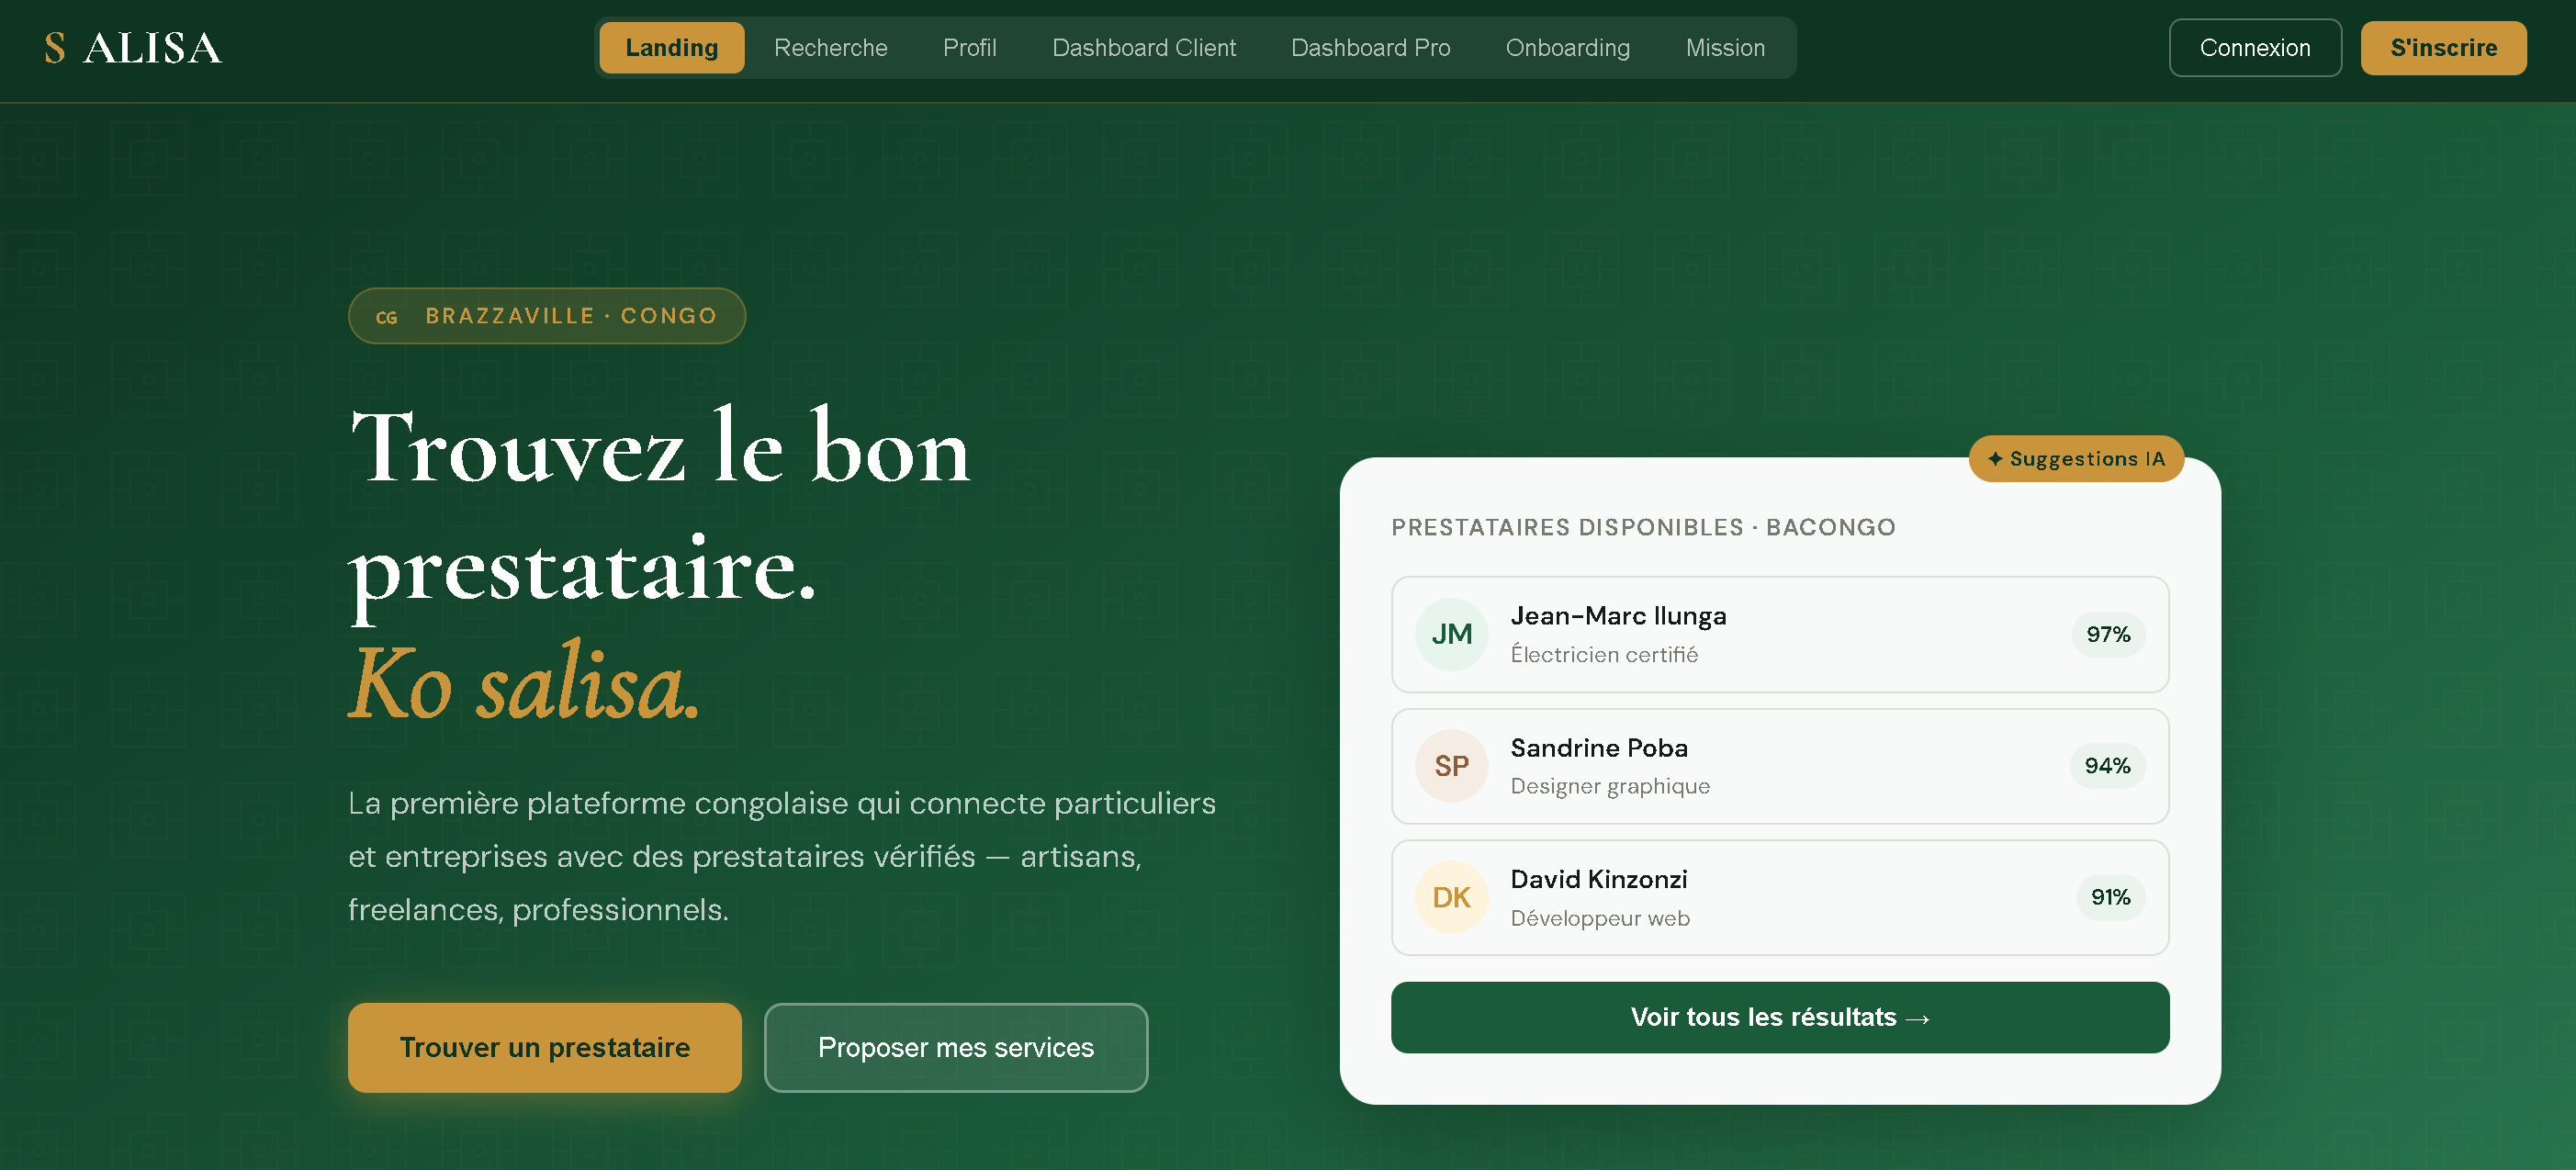
\includegraphics[width=0.85\textwidth, height=9.5cm, keepaspectratio=false]{captures_appli/capture_accueil.png}
	\caption{Page d'accueil de l'application « SALISA »}
	\label{fig:cap_accueil}
\end{figure}

\begin{figure}[H]
	\centering
	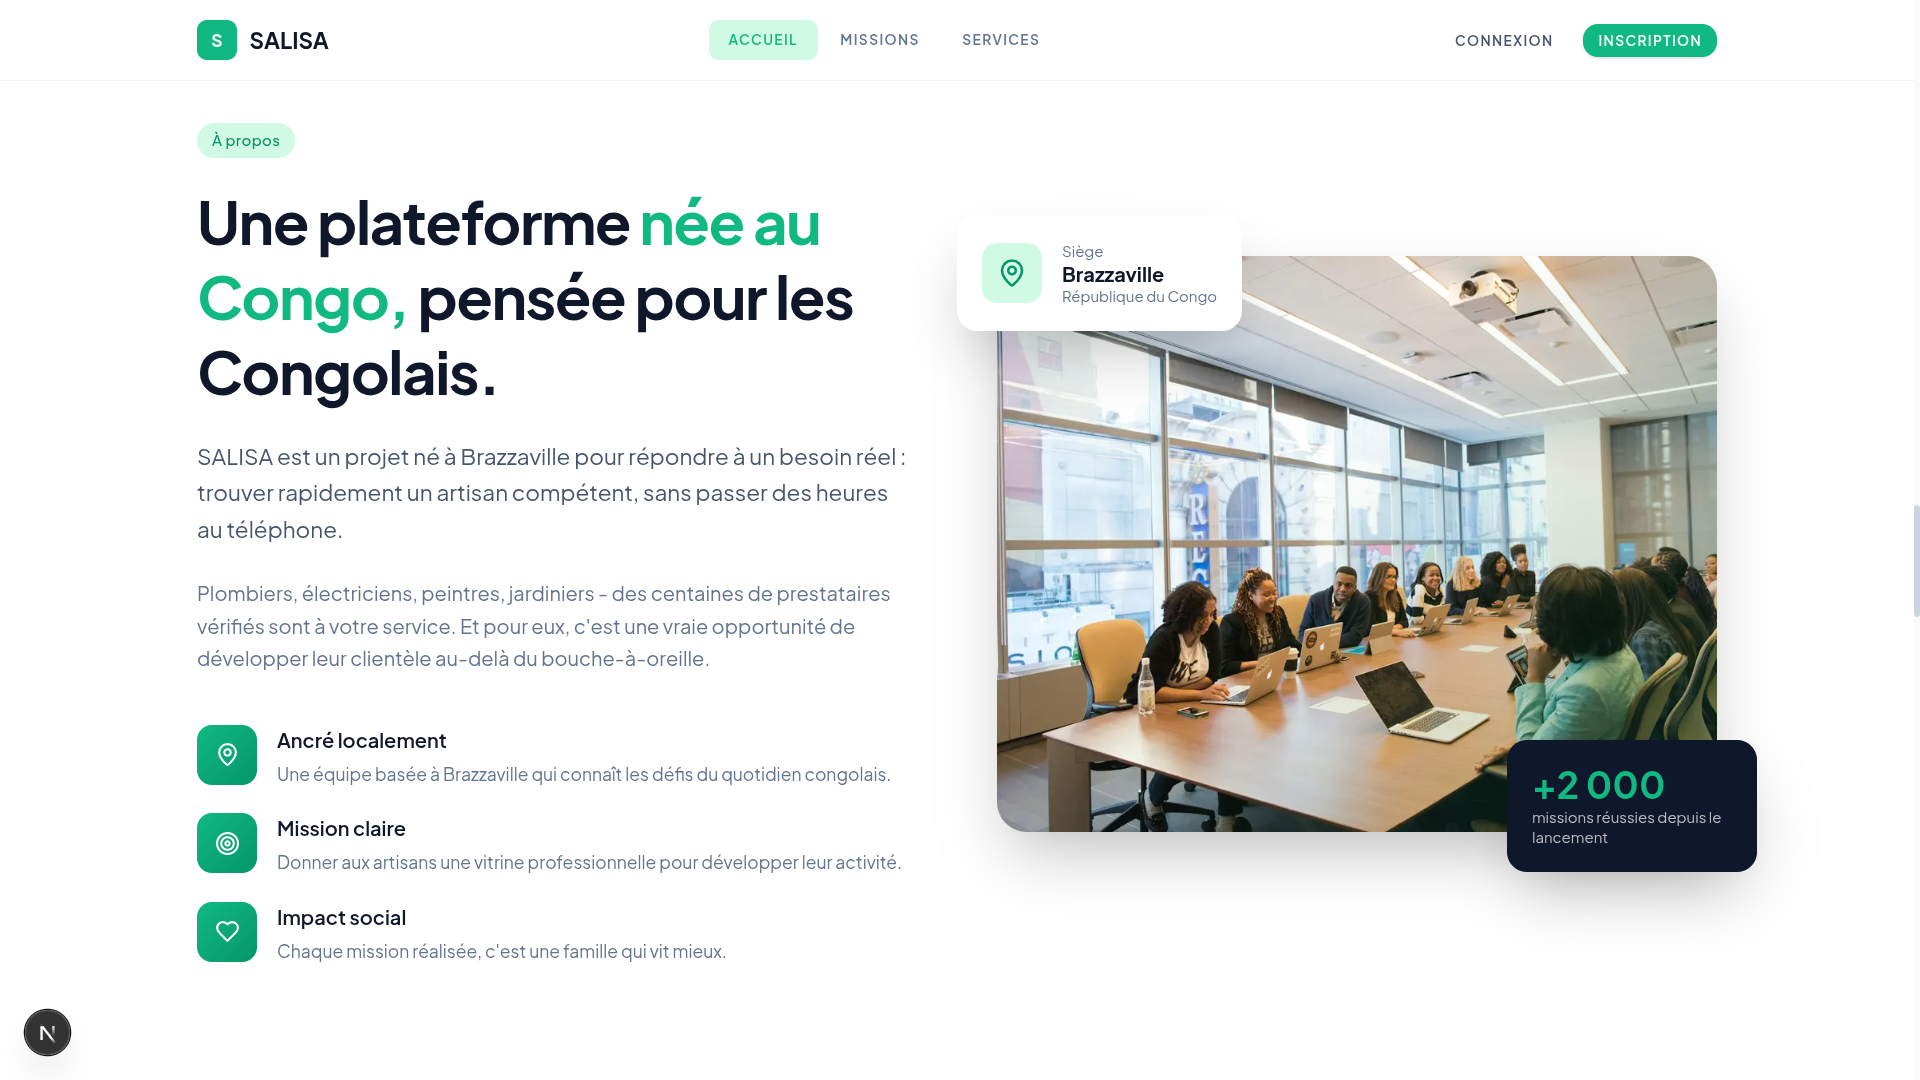
\includegraphics[width=0.85\textwidth, height=9.5cm, keepaspectratio=false]{captures_appli/capture_landing.png}
	\caption{Landing page de l'application « SALISA »}
	\label{fig:cap_landing}
\end{figure}

\begin{figure}[H]
	\centering
	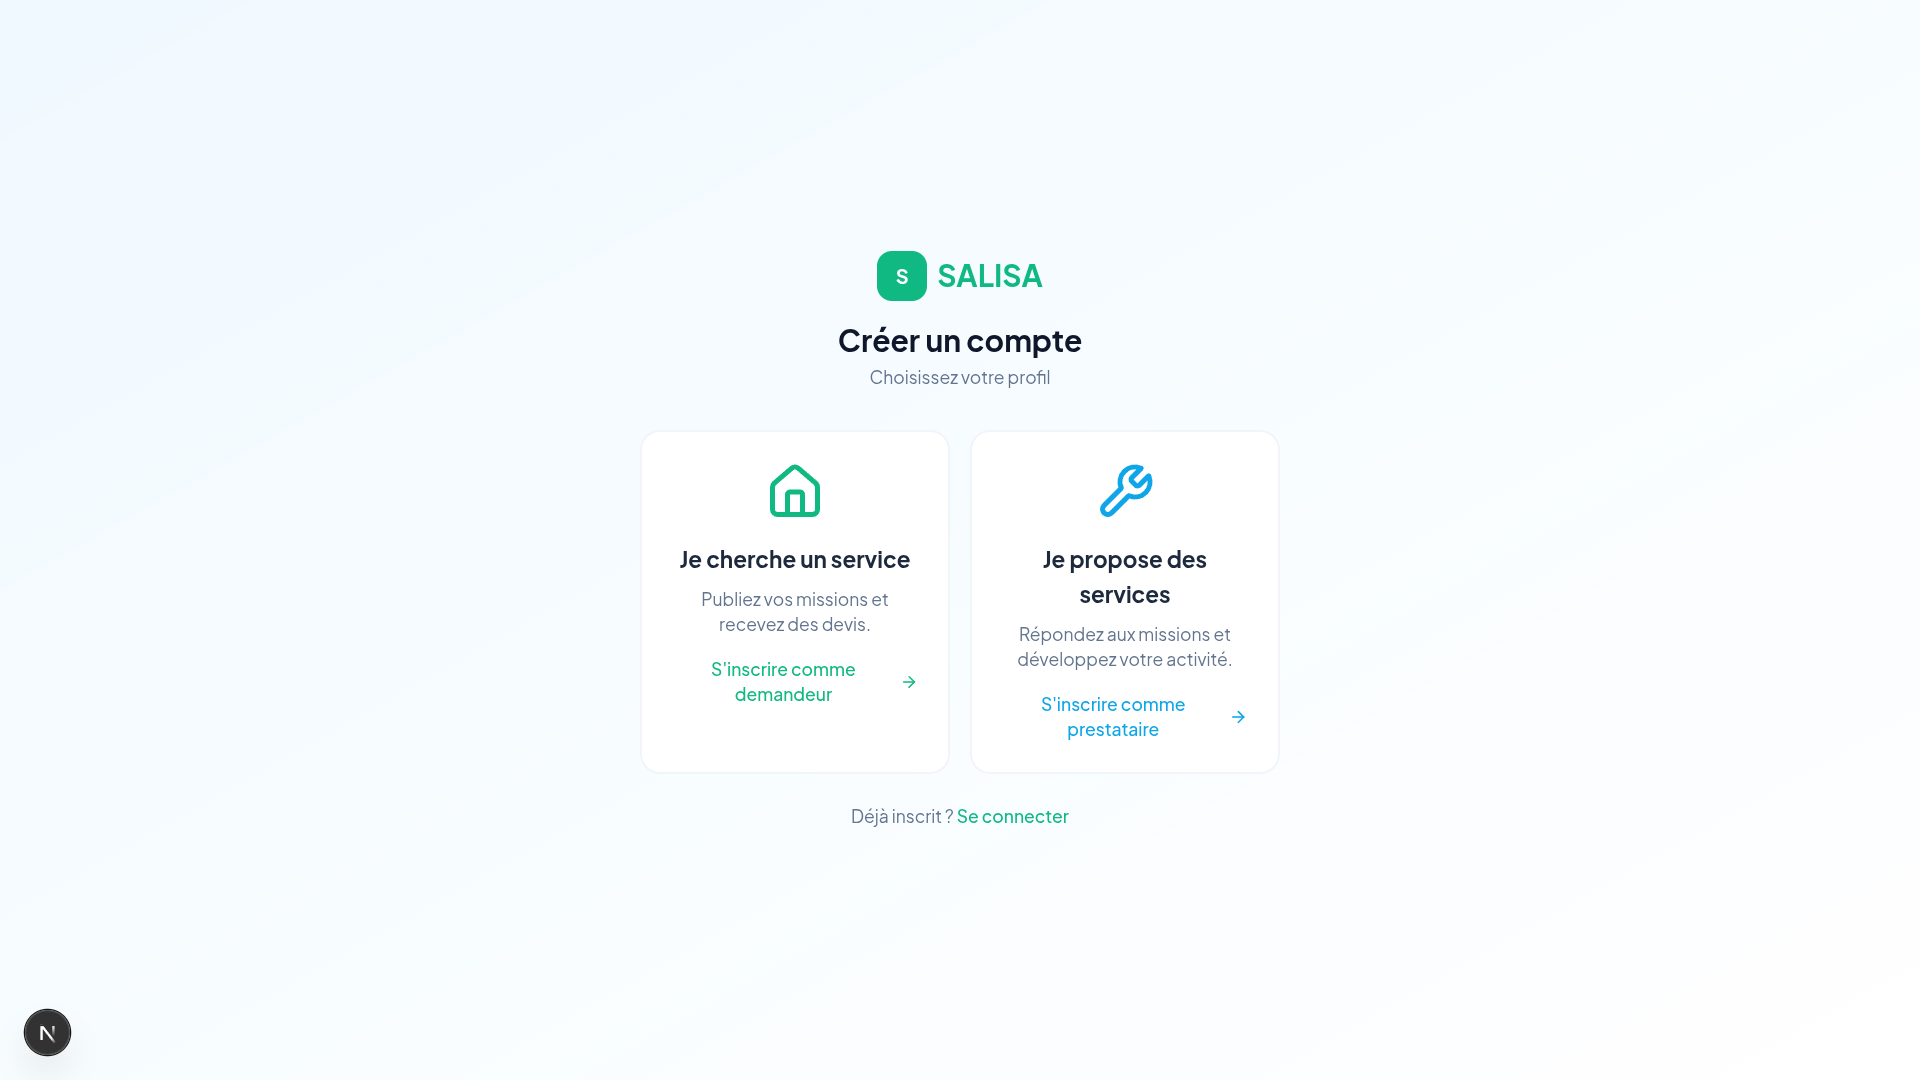
\includegraphics[width=0.85\textwidth, height=9.5cm, keepaspectratio=false]{captures_appli/capture_choix_role.png}
	\caption{Écran de choix du rôle lors de l'inscription}
	\label{fig:cap_role}
\end{figure}

\begin{figure}[H]
	\centering
	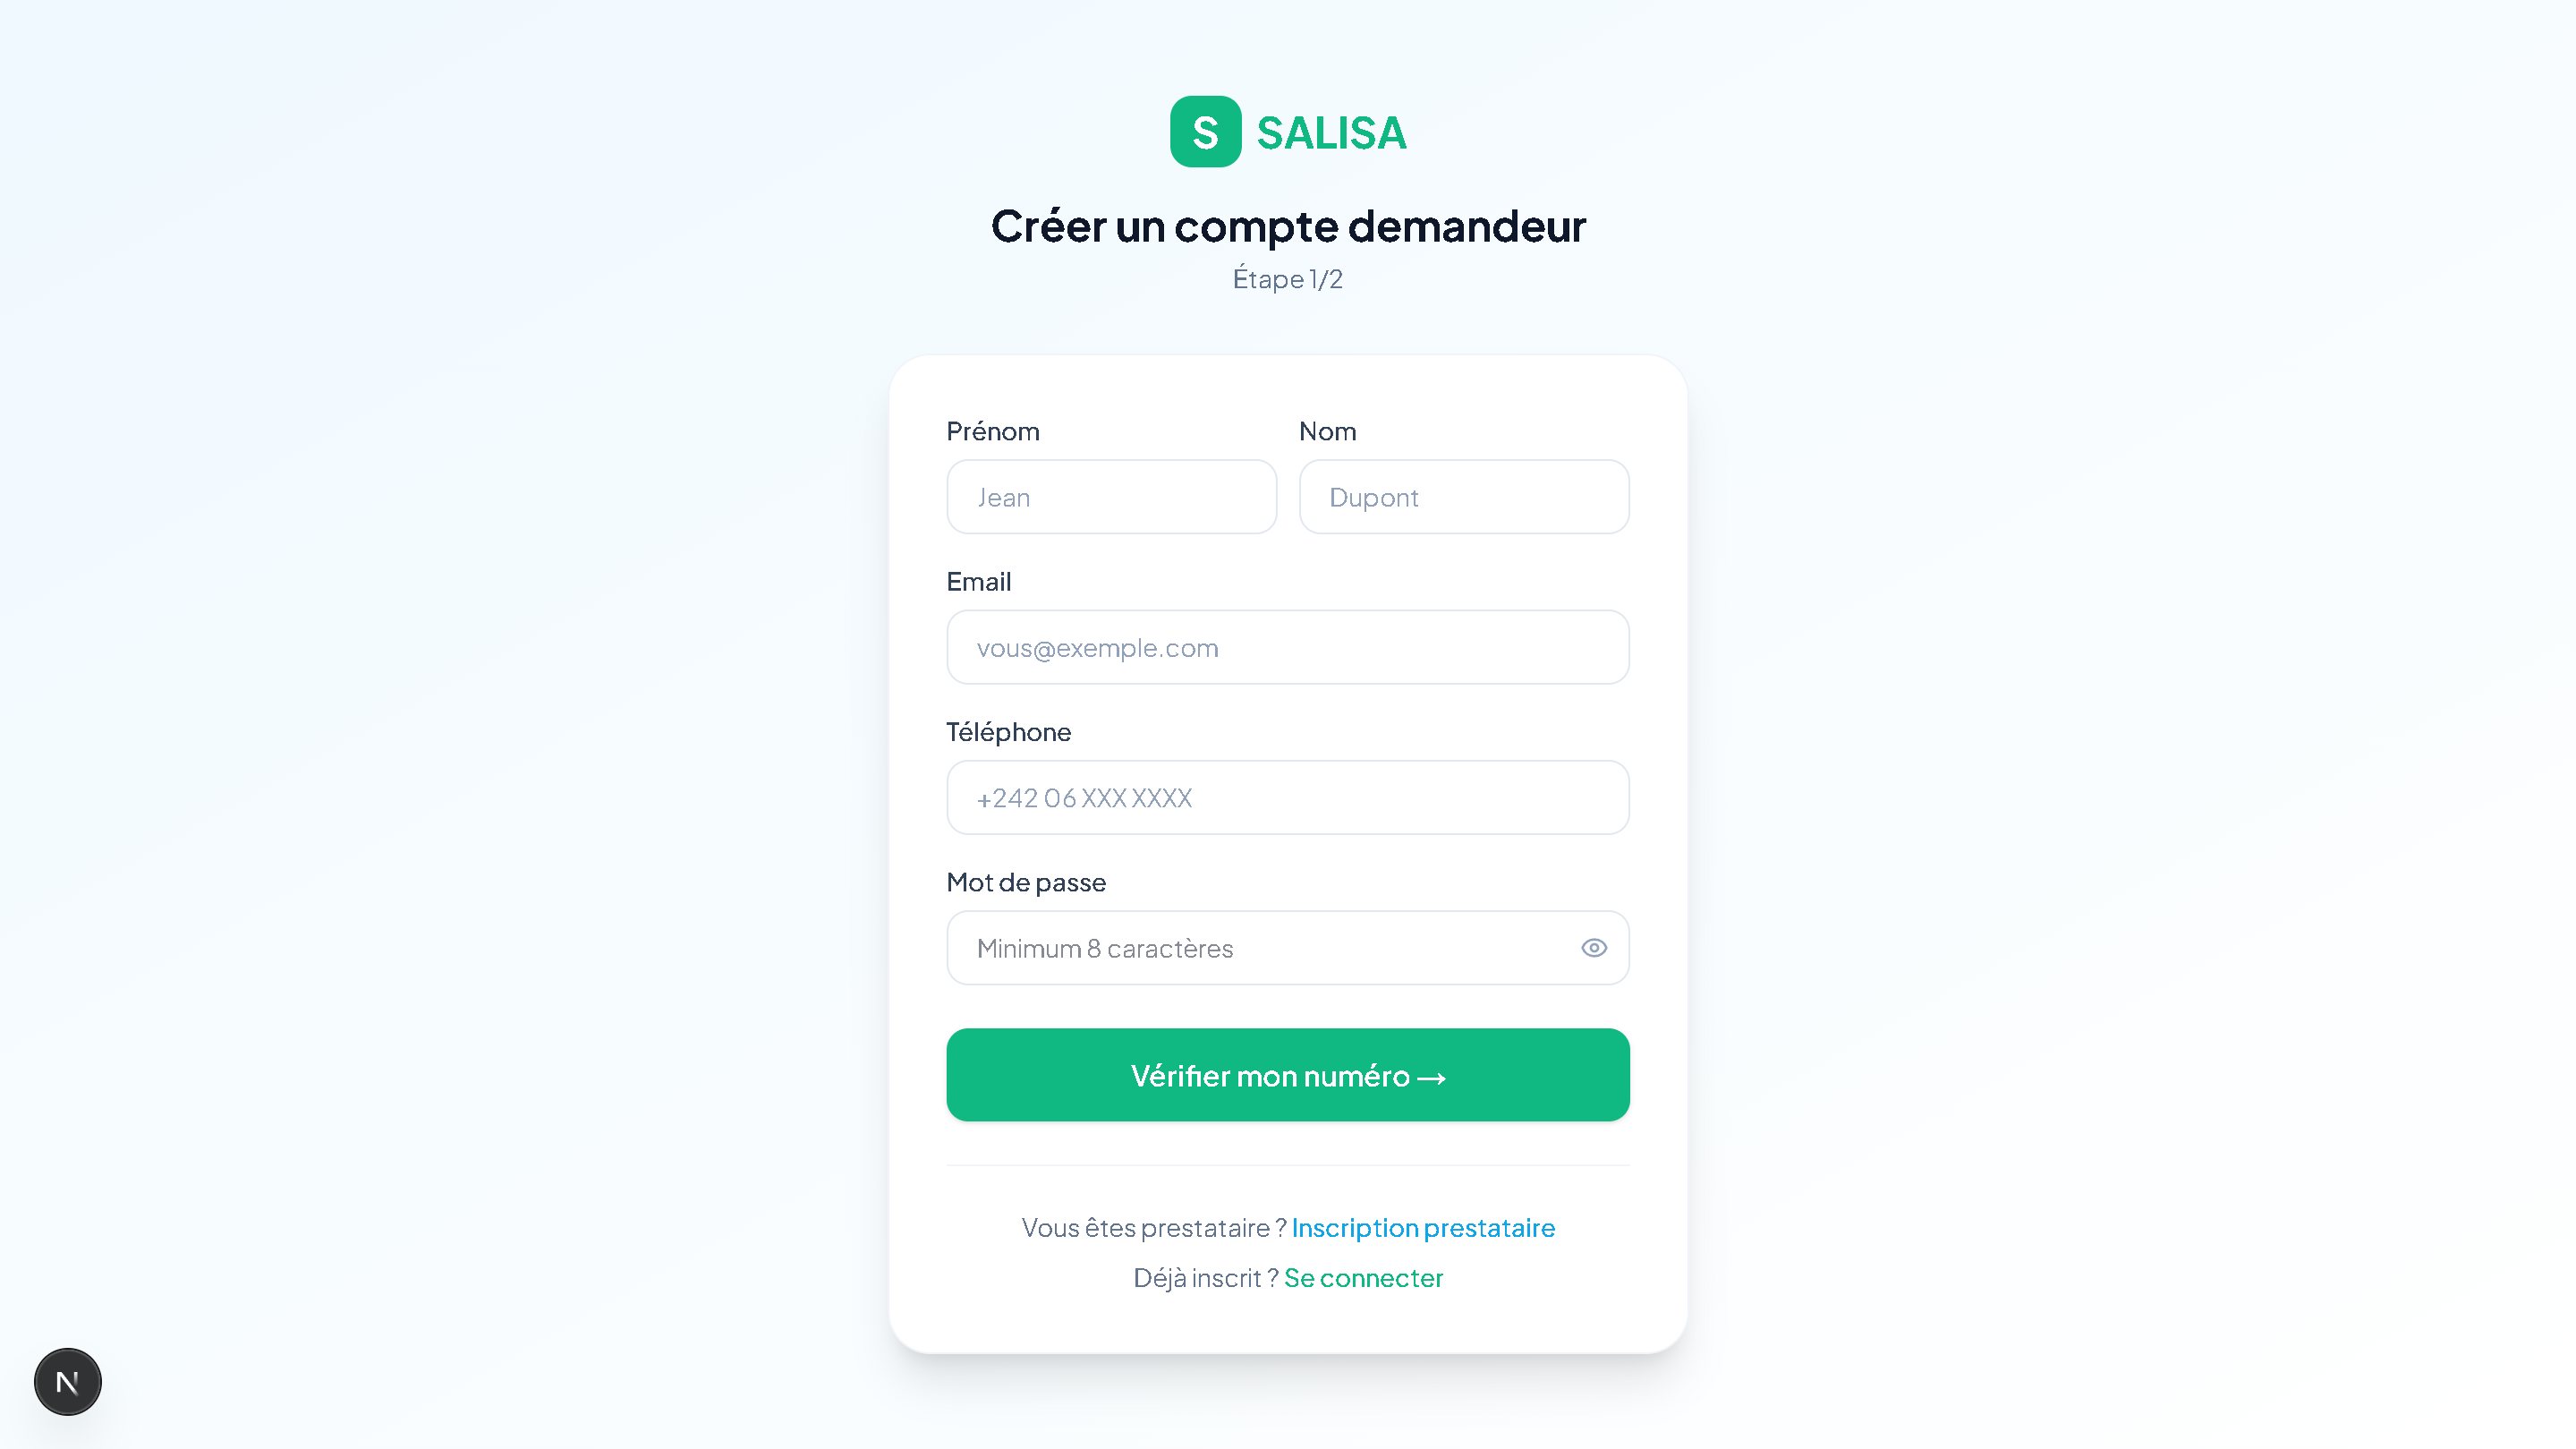
\includegraphics[width=0.85\textwidth, height=9.5cm, keepaspectratio=false]{captures_appli/capture_inscription.png}
	\caption{Écran d'inscription via numéro de téléphone}
	\label{fig:cap_inscription}
\end{figure}

\begin{figure}[H]
	\centering
	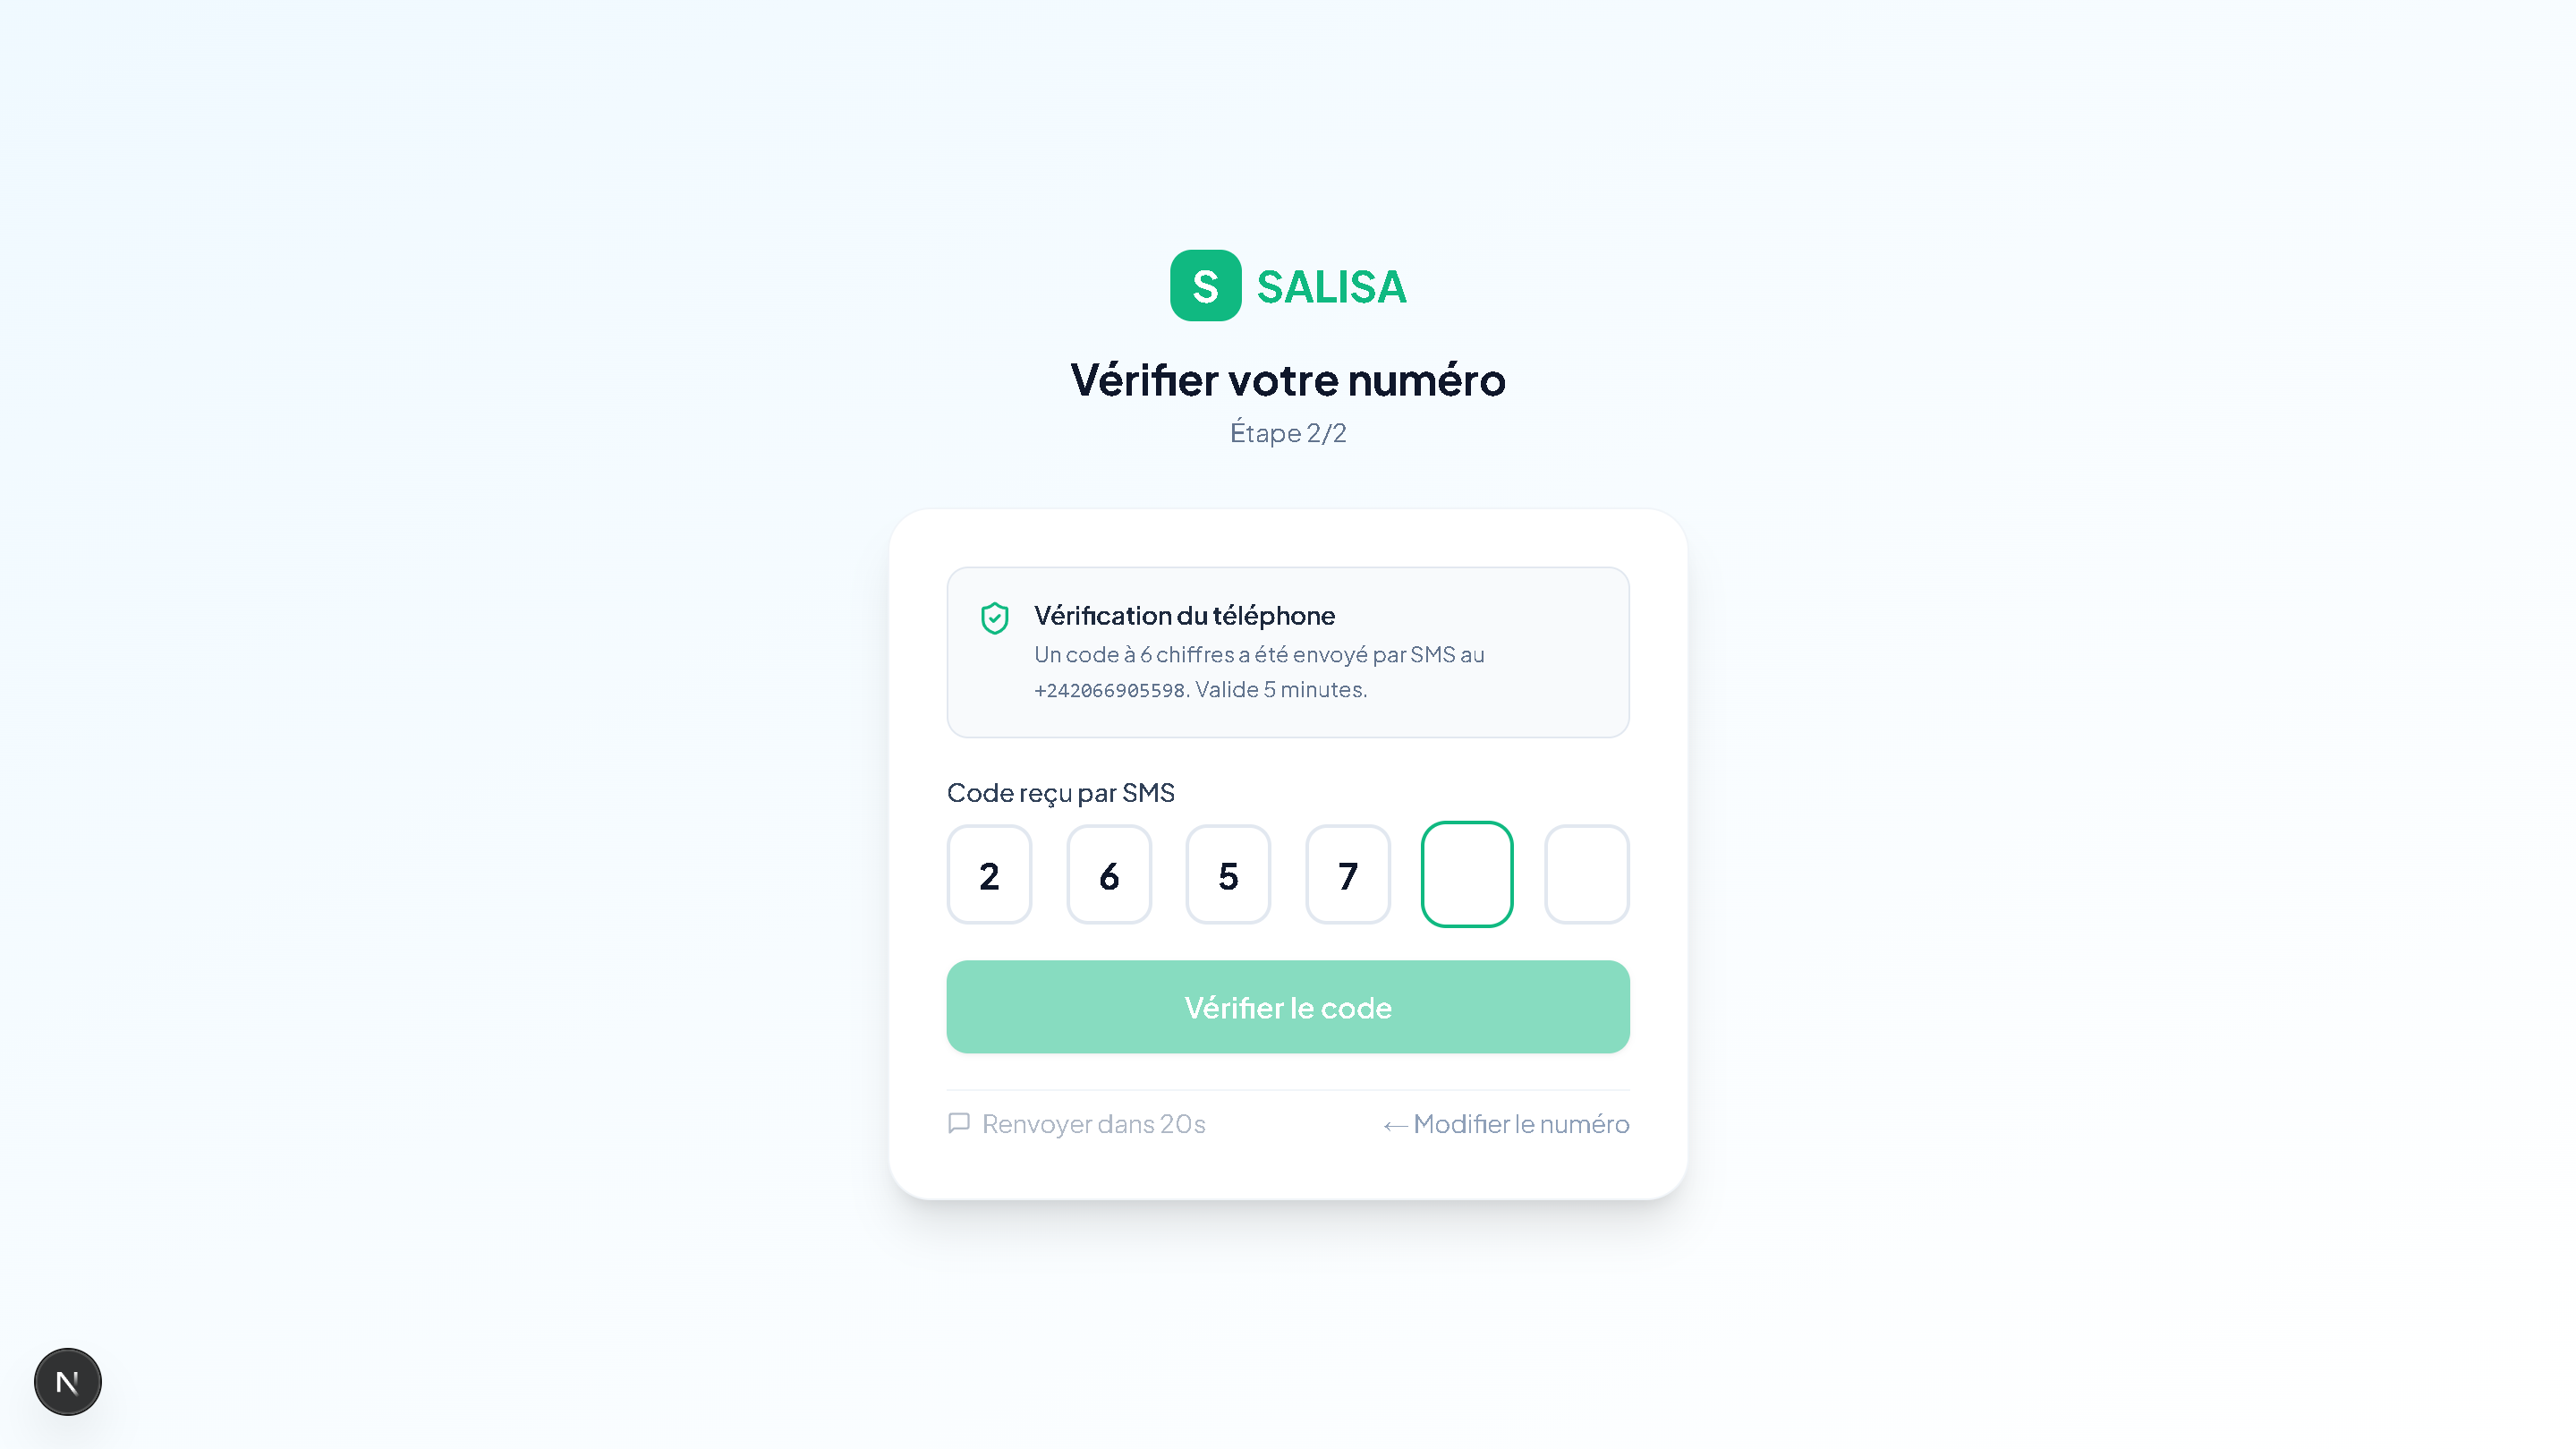
\includegraphics[width=0.85\textwidth, height=9.5cm, keepaspectratio=false]{captures_appli/capture_otp.png}
	\caption{Écran de validation du code OTP}
	\label{fig:cap_otp}
\end{figure}

\begin{figure}[H]
	\centering
	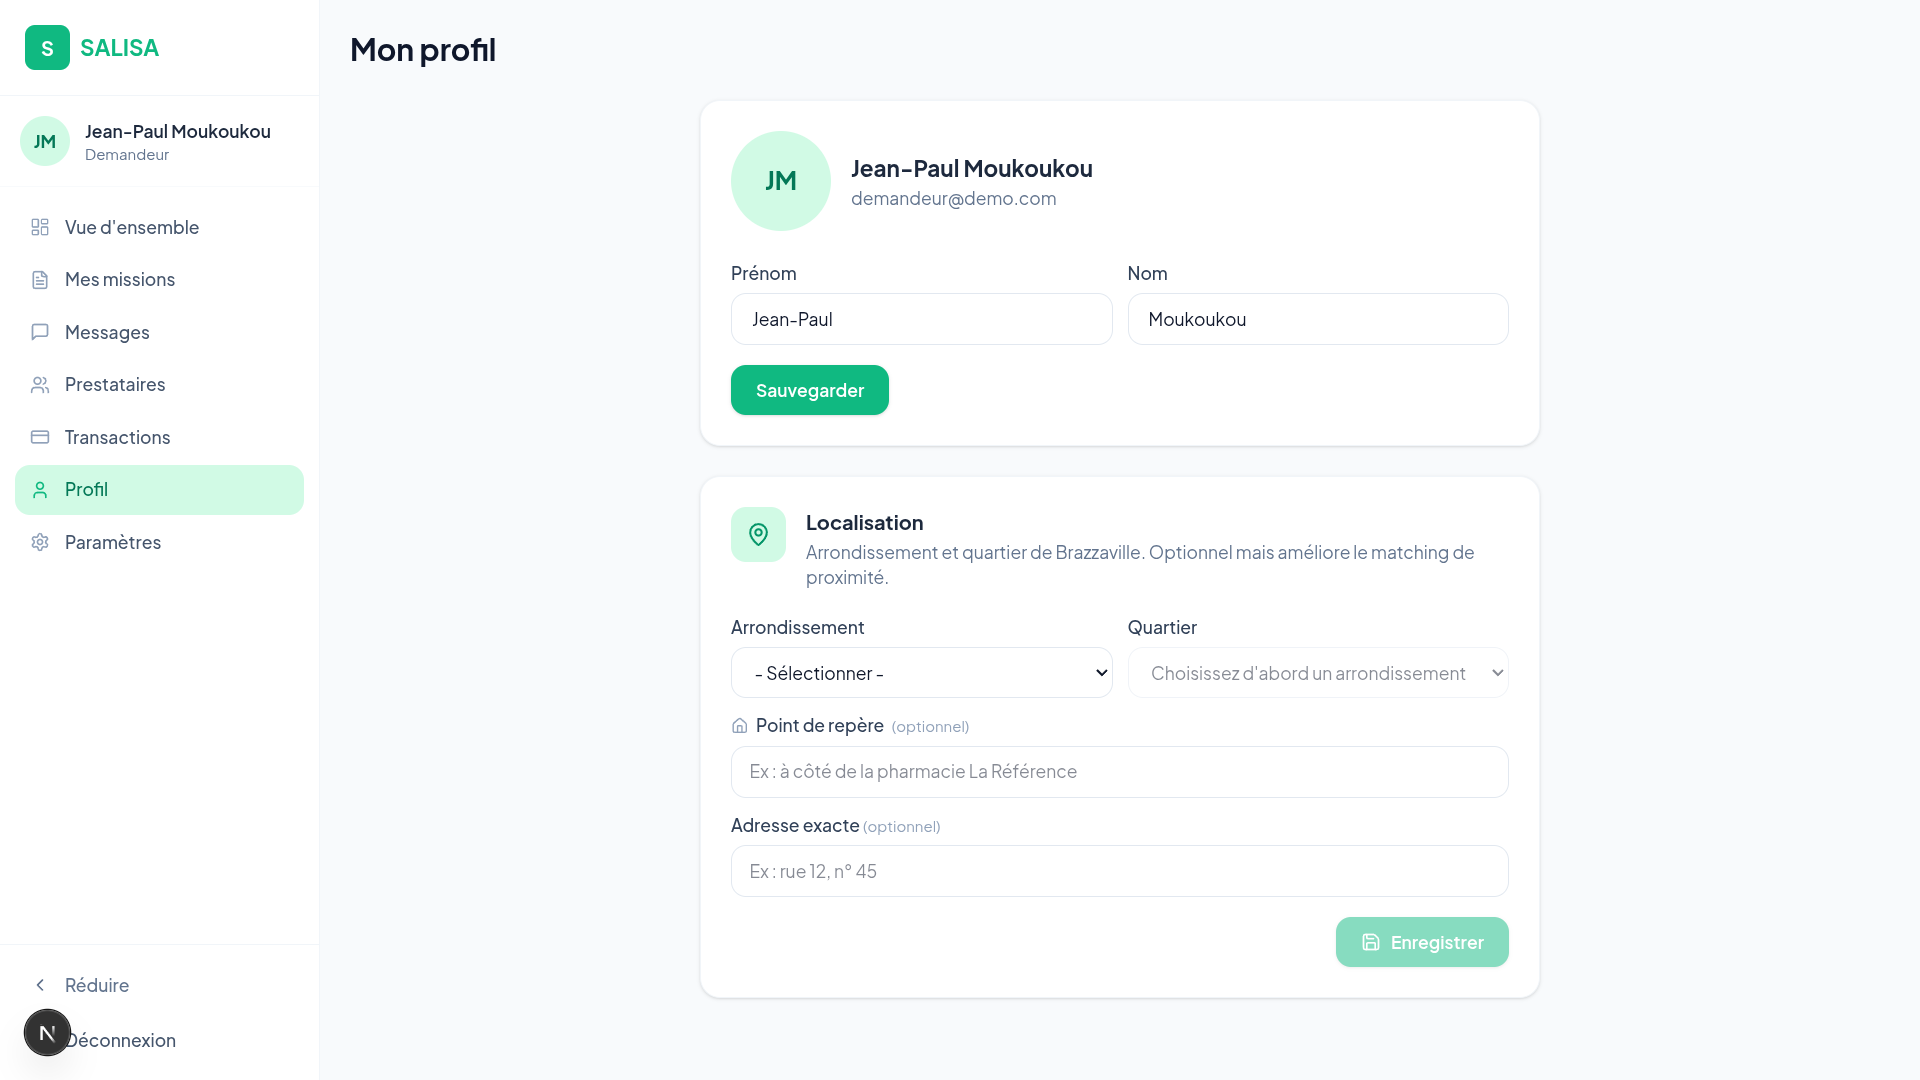
\includegraphics[width=0.85\textwidth, height=9.5cm, keepaspectratio=false]{captures_appli/capture_profil_demandeur.png}
	\caption{Profil du demandeur}
	\label{fig:cap_profil_demandeur}
\end{figure}

\begin{figure}[H]
	\centering
	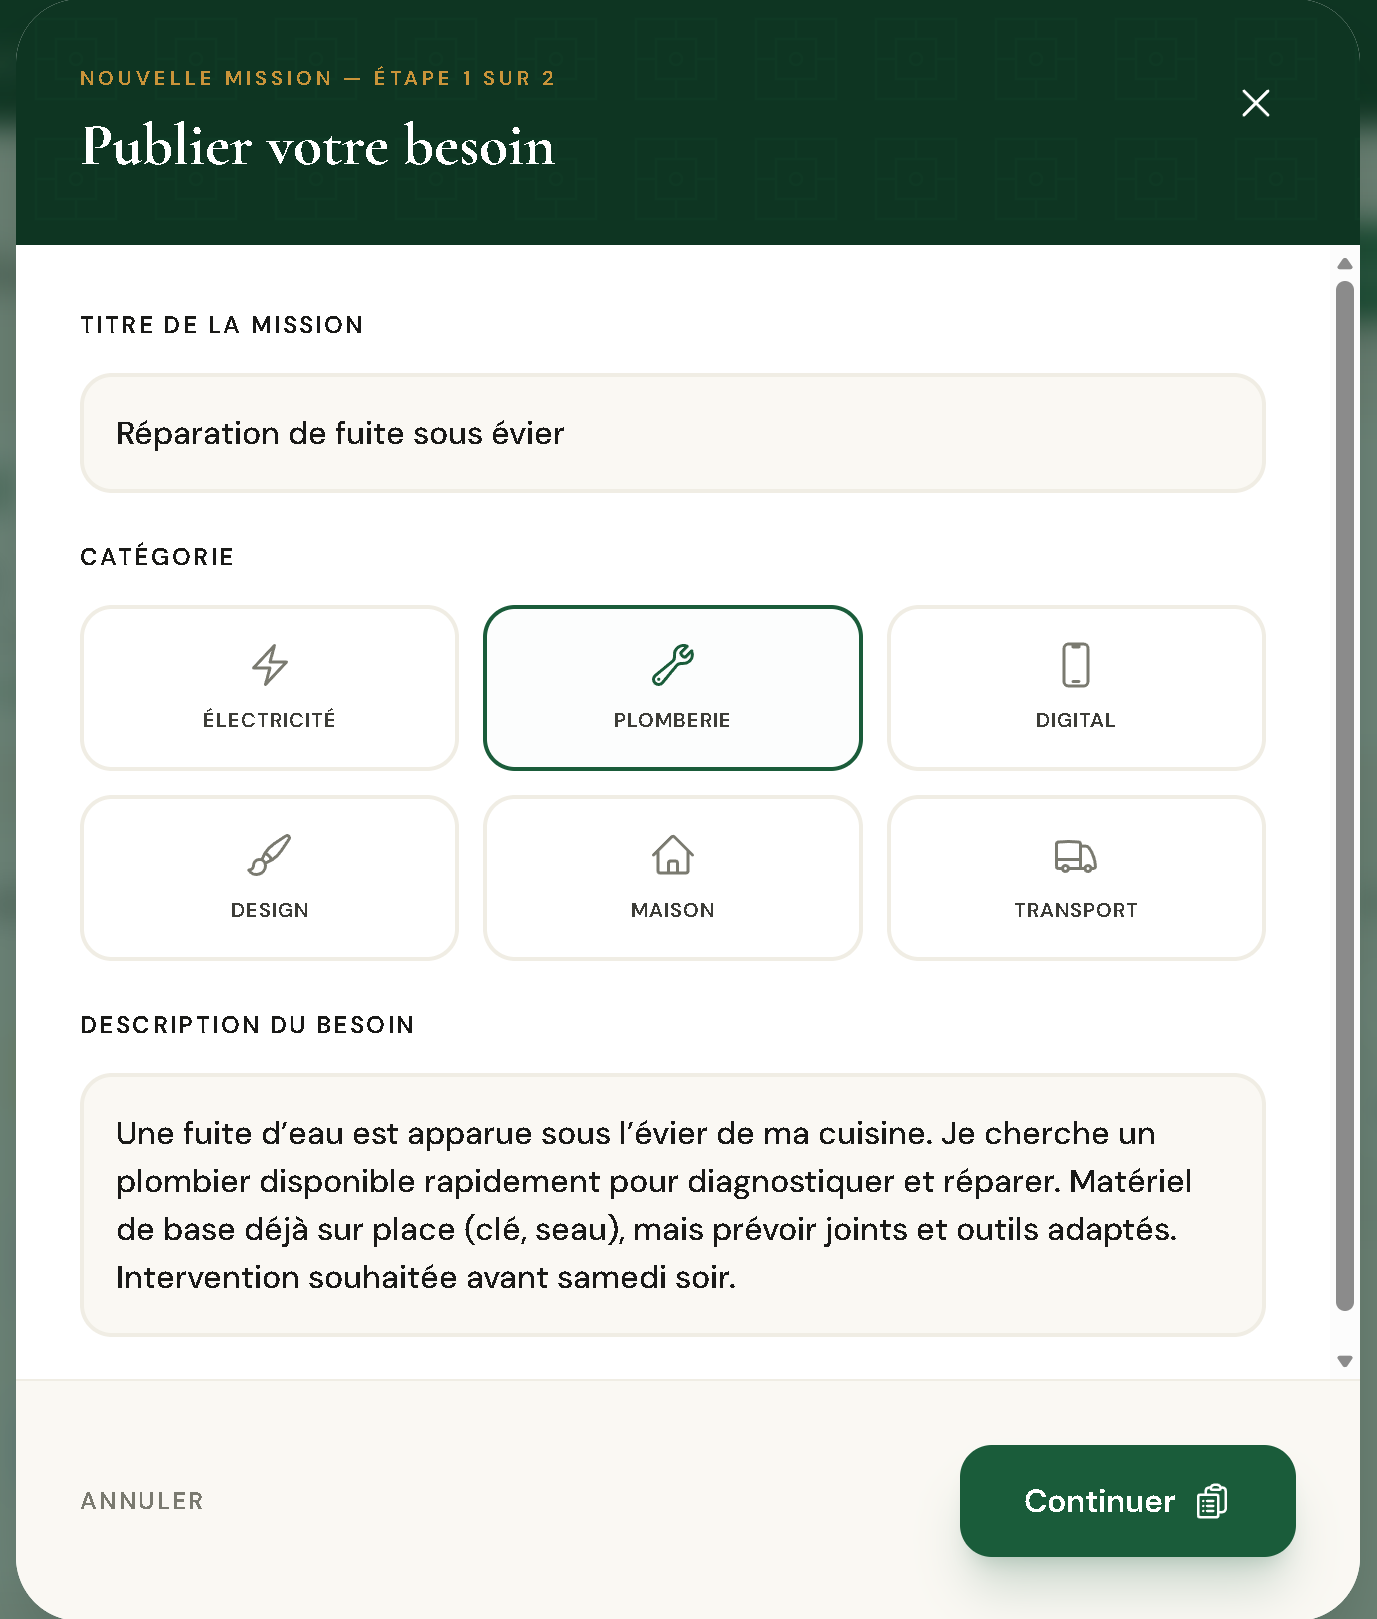
\includegraphics[width=0.85\textwidth, height=9.5cm, keepaspectratio=false]{captures_appli/capture_publication_mission.png}
	\caption{Formulaire de publication d'une mission}
	\label{fig:cap_publication}
\end{figure}

\begin{figure}[H]
	\centering
	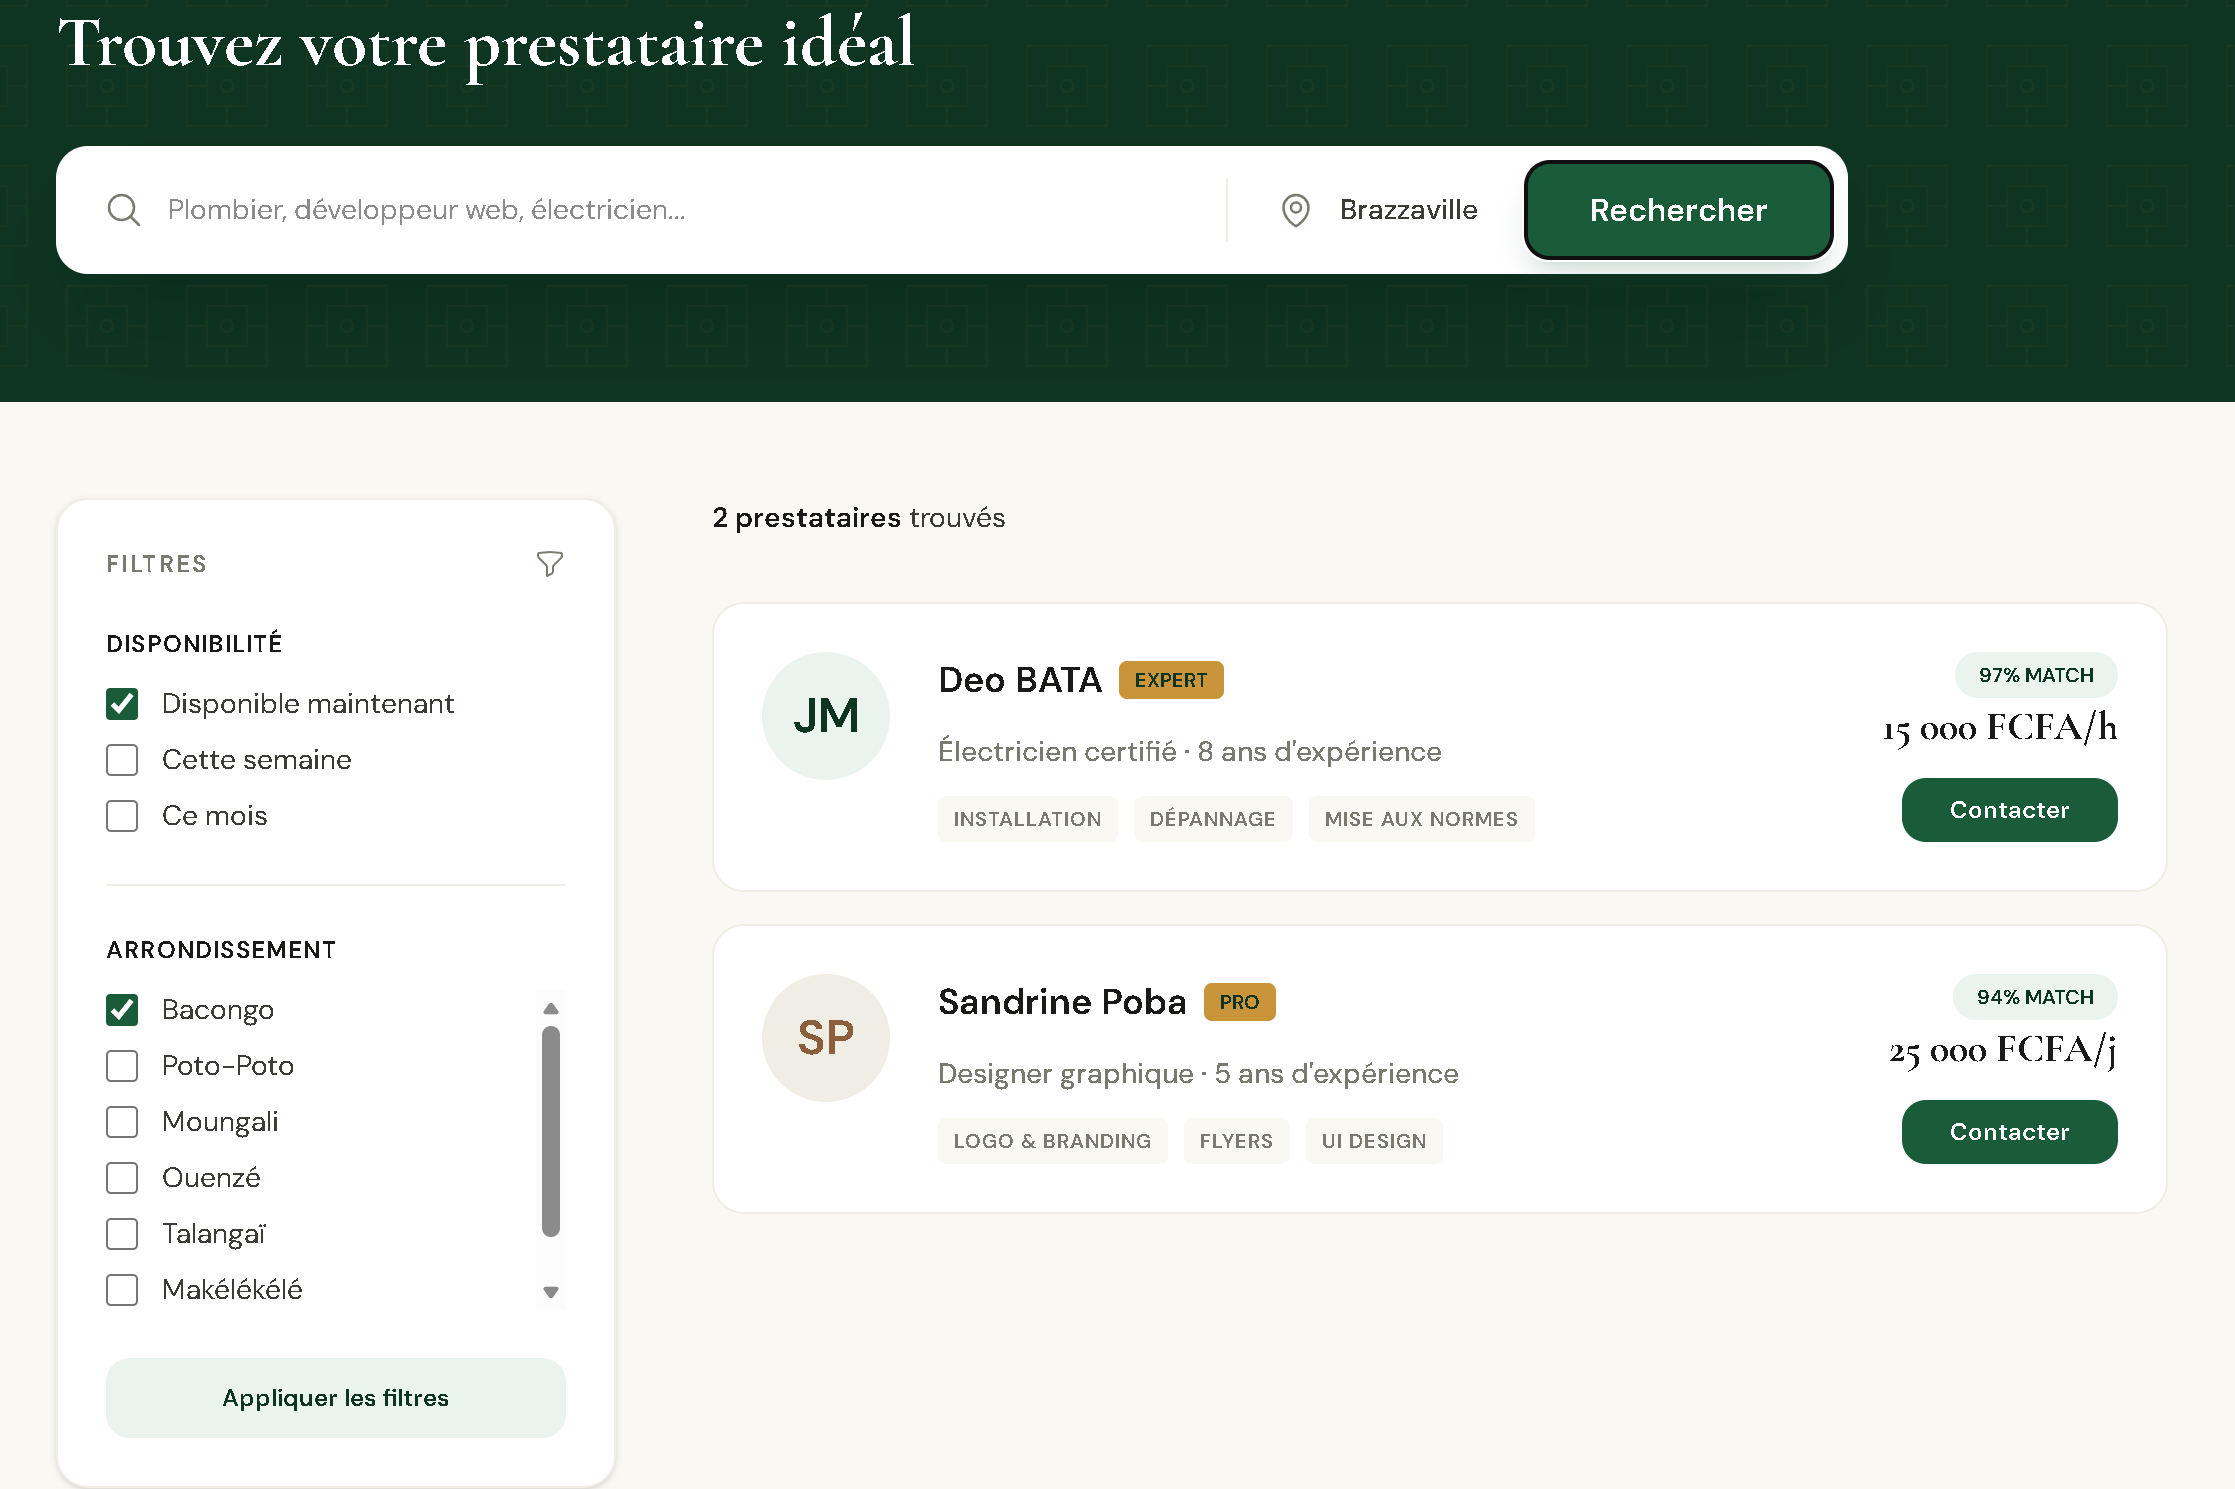
\includegraphics[width=0.85\textwidth, height=9.5cm, keepaspectratio=false]{captures_appli/capture_recherche_prestataires.png}
	\caption{Résultats de recherche de prestataires}
	\label{fig:cap_recherche}
\end{figure}

\begin{figure}[H]
	\centering
	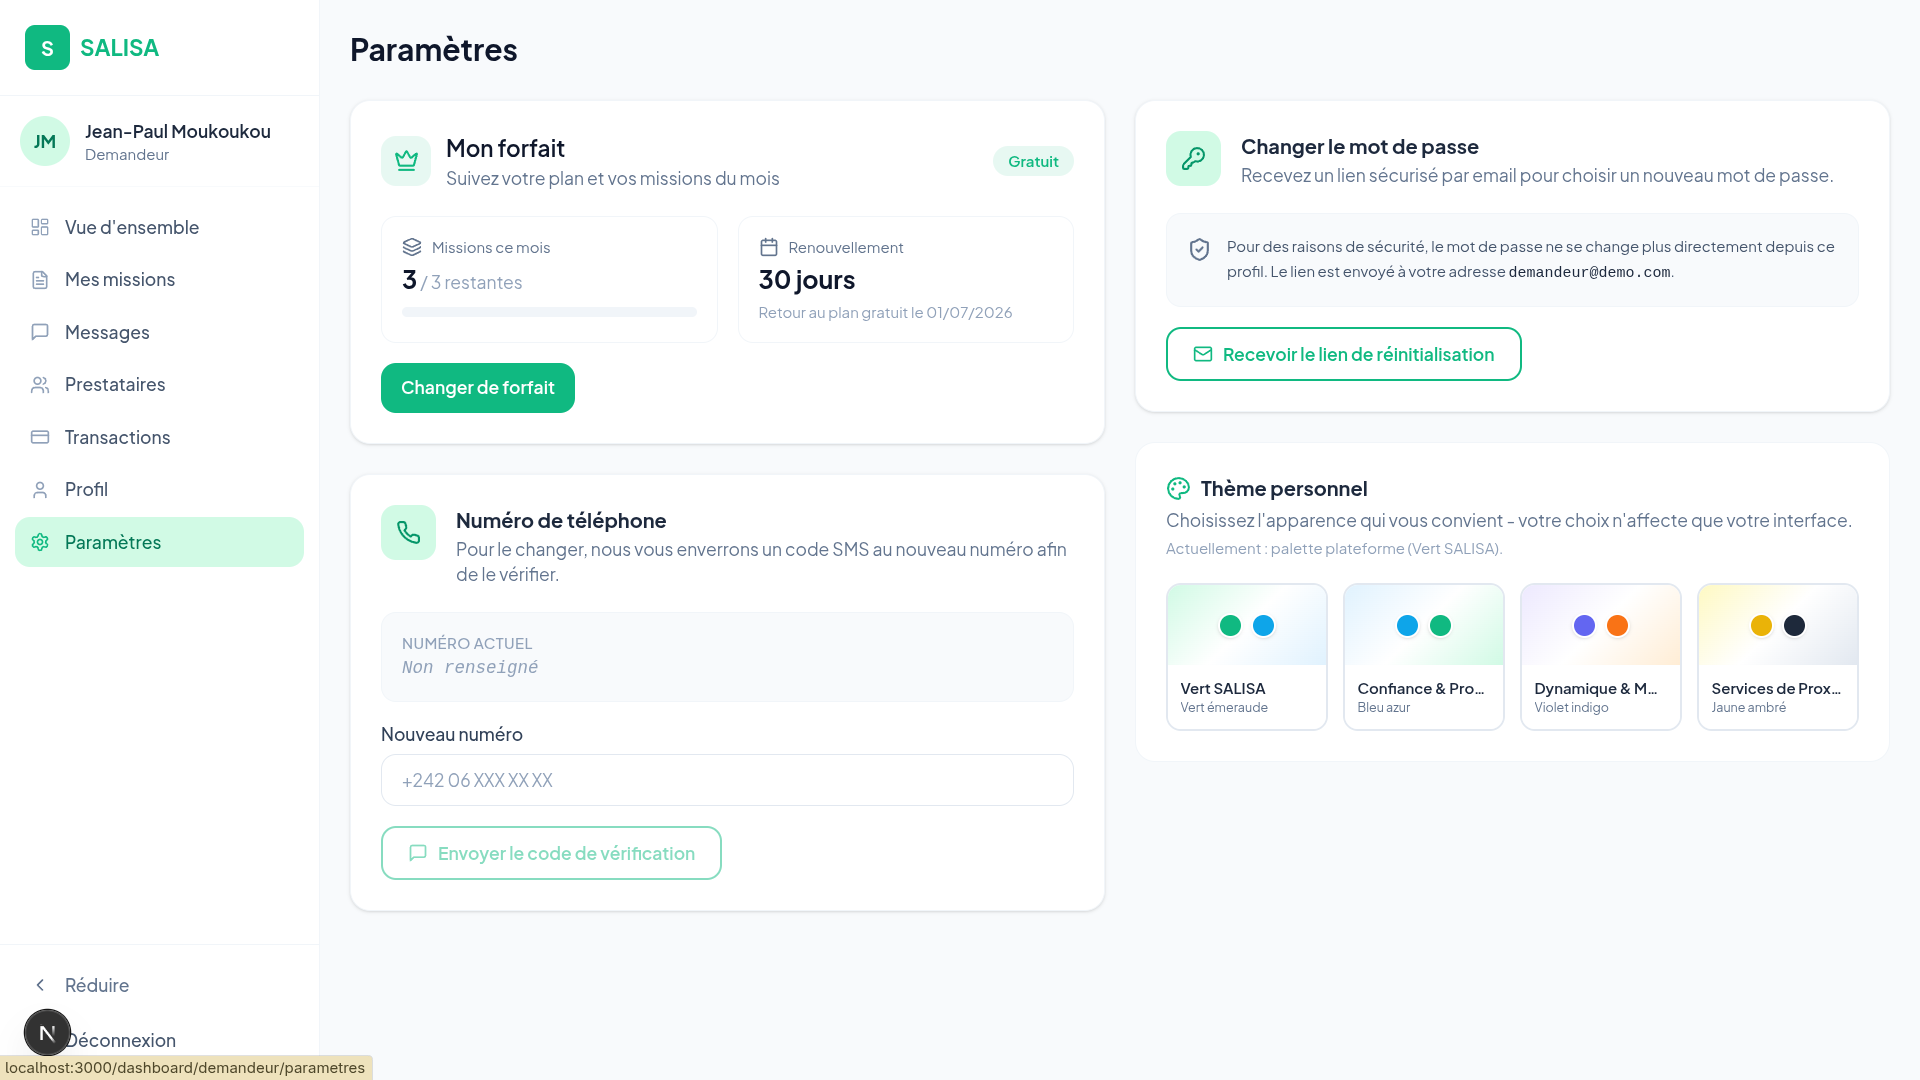
\includegraphics[width=0.85\textwidth, height=9.5cm, keepaspectratio=false]{captures_appli/captures_gestion_parametres.png}
	\caption{Gestion des paramètres}
	\label{fig:cap_parametre}
\end{figure}


%\begin{figure}[H]
%    \centering
%    \includegraphics[width=0.85\textwidth, height=9.5cm, keepaspectratio=false]{captures_appli/capture_paiement.png}
%    \caption{Écran de paiement via MTN MoMo ou Airtel Money}
%    \label{fig:cap_paiement}
%\end{figure}

\begin{figure}[H]
	\centering
	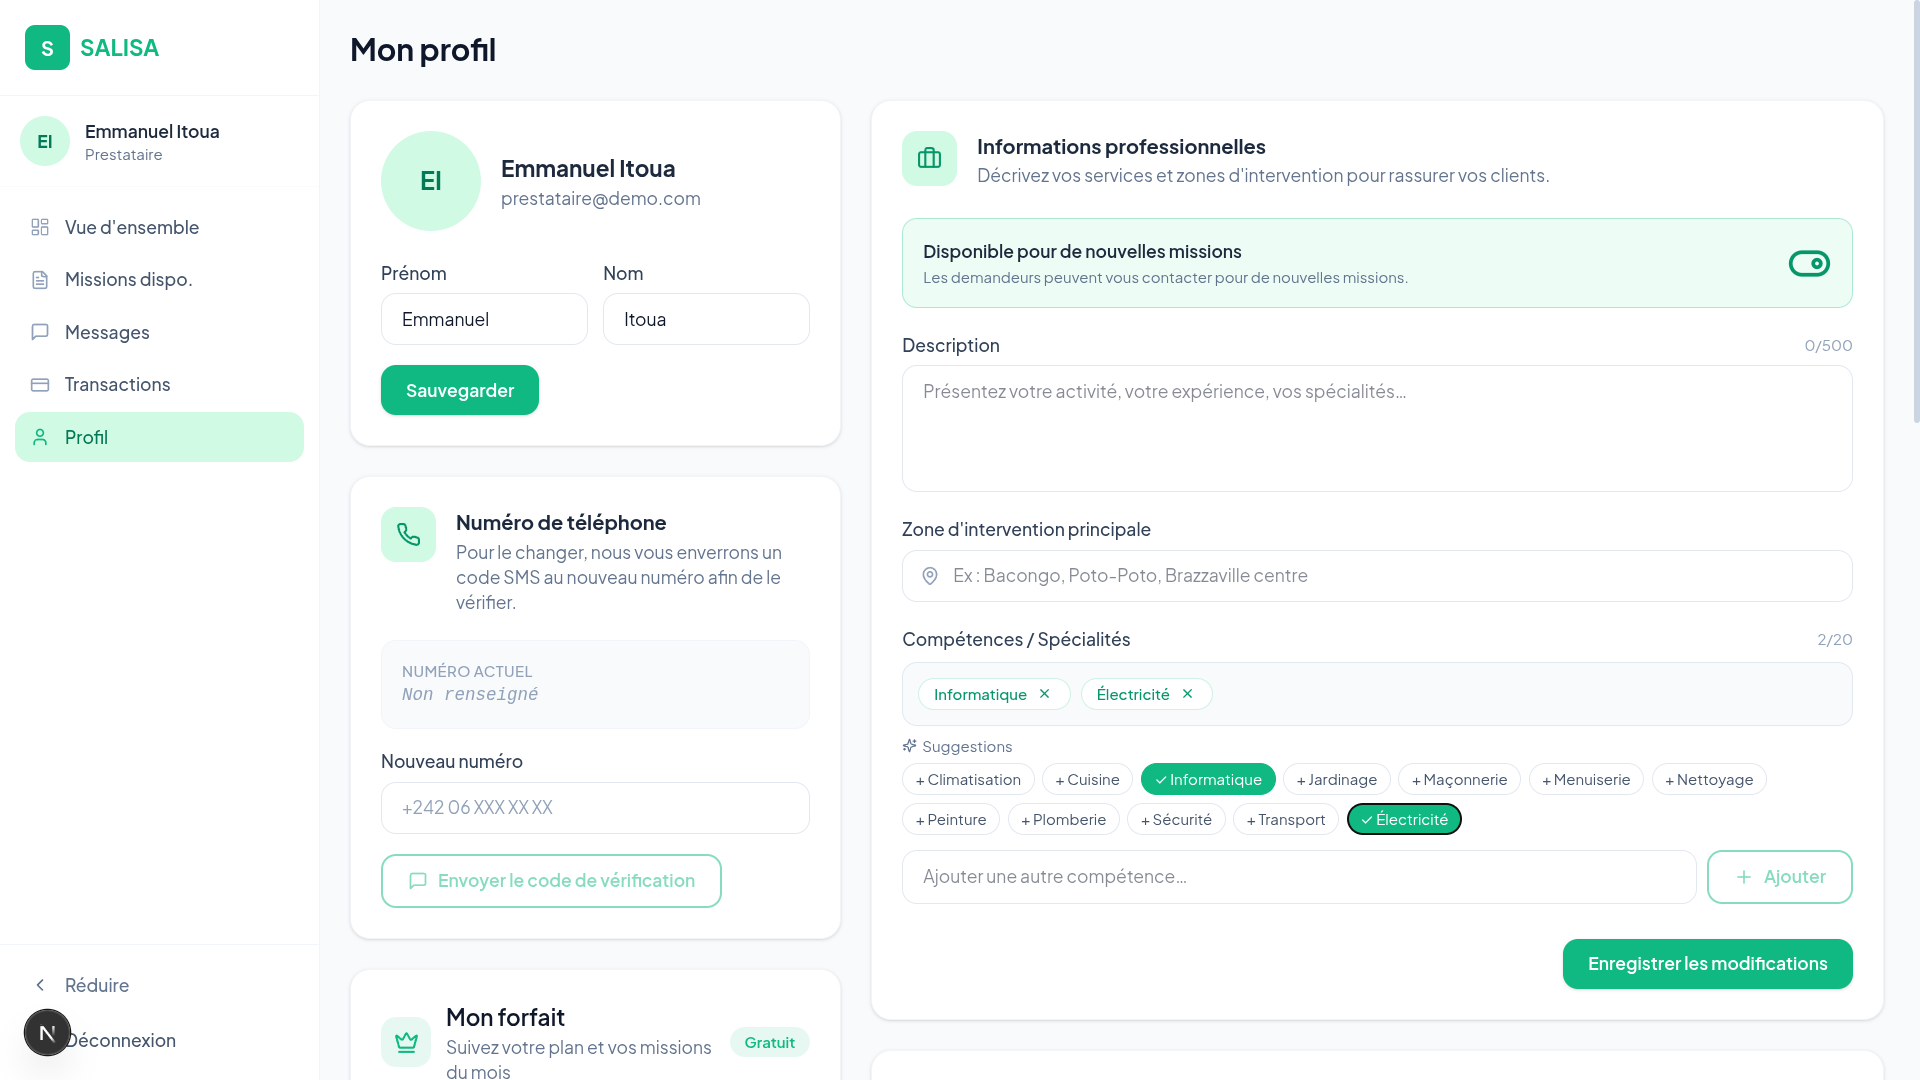
\includegraphics[width=0.85\textwidth, height=9.5cm, keepaspectratio=false]{captures_appli/capture_profil_prestatire.png}
	\caption{Profil du prestataire}
	\label{fig:cap_profil_prestataire}
\end{figure}

\begin{figure}[H]
	\centering
	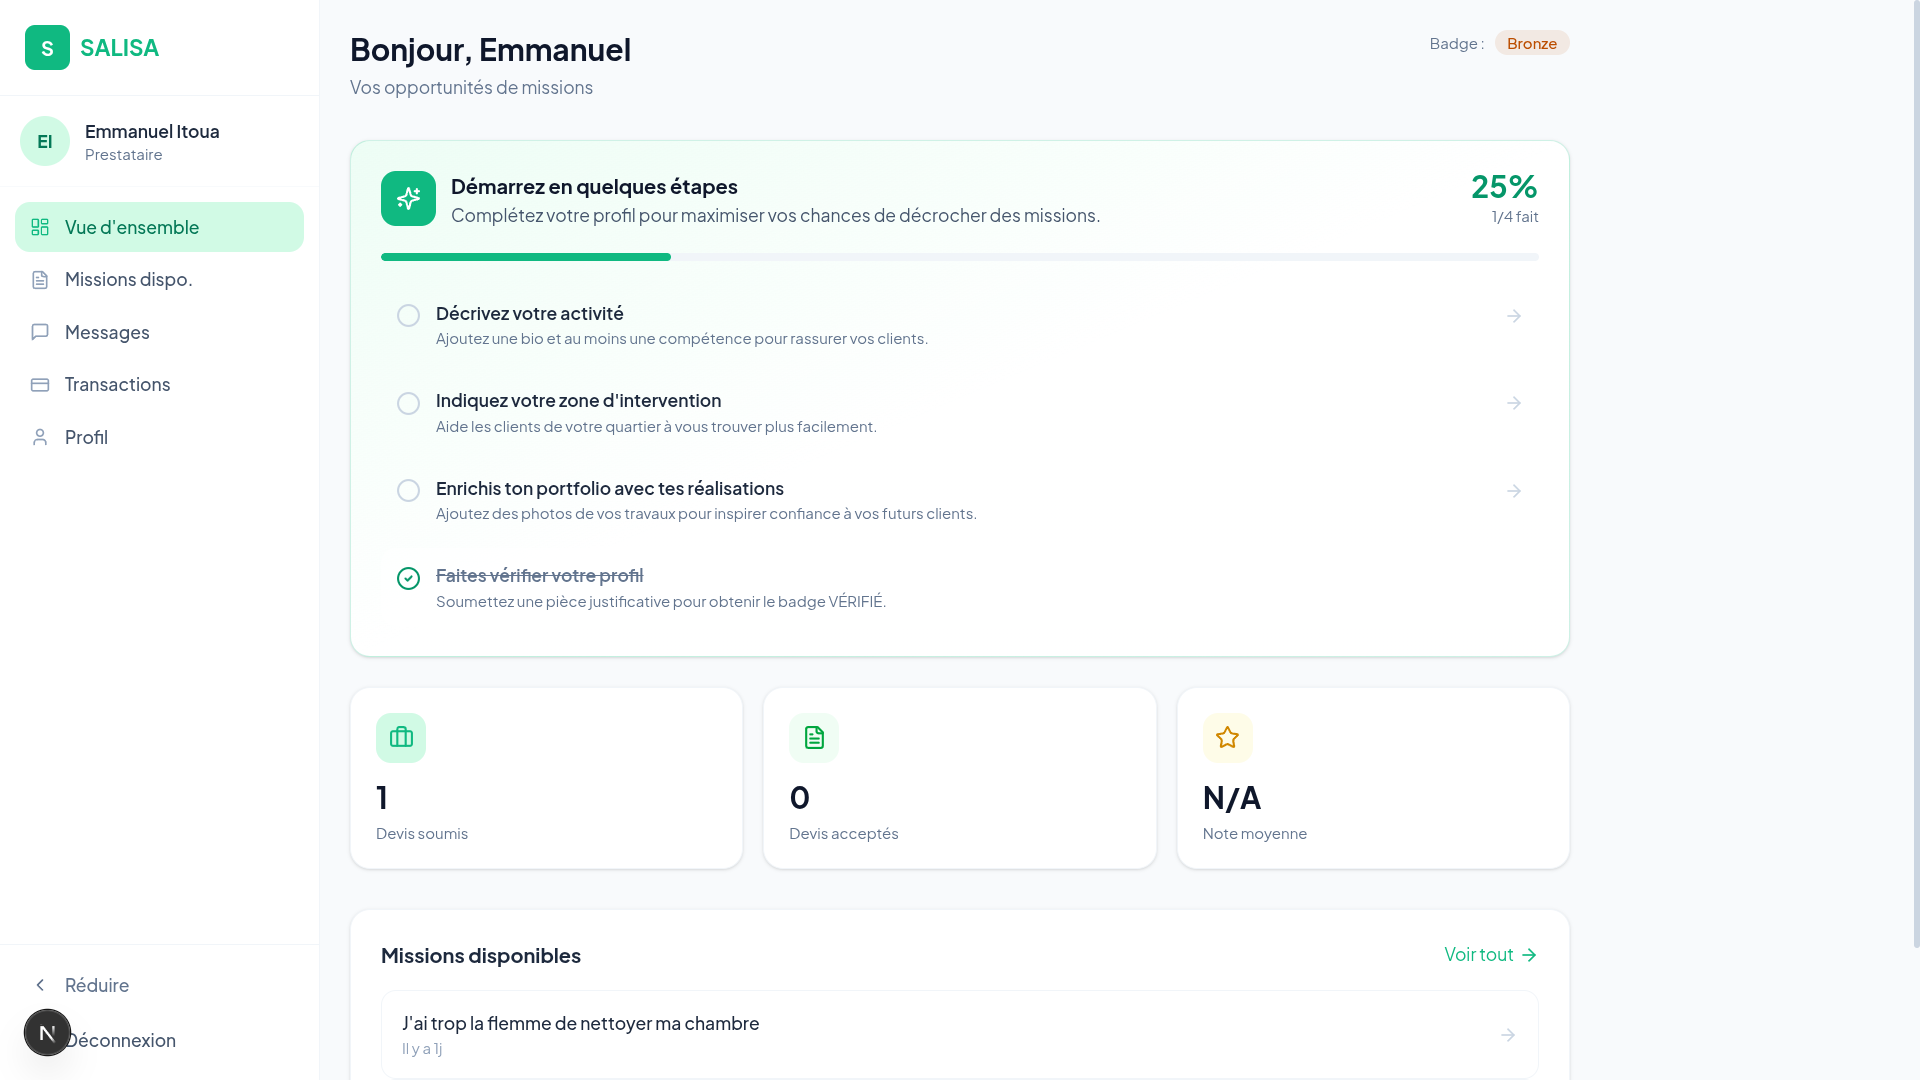
\includegraphics[width=0.85\textwidth, height=9.5cm, keepaspectratio=false]{captures_appli/capture_completion_profil.png}
	\caption{Complétion du profil prestataire}
	\label{fig:cap_complete_profil_prestataire}
\end{figure}

\begin{figure}[H]
	\centering
	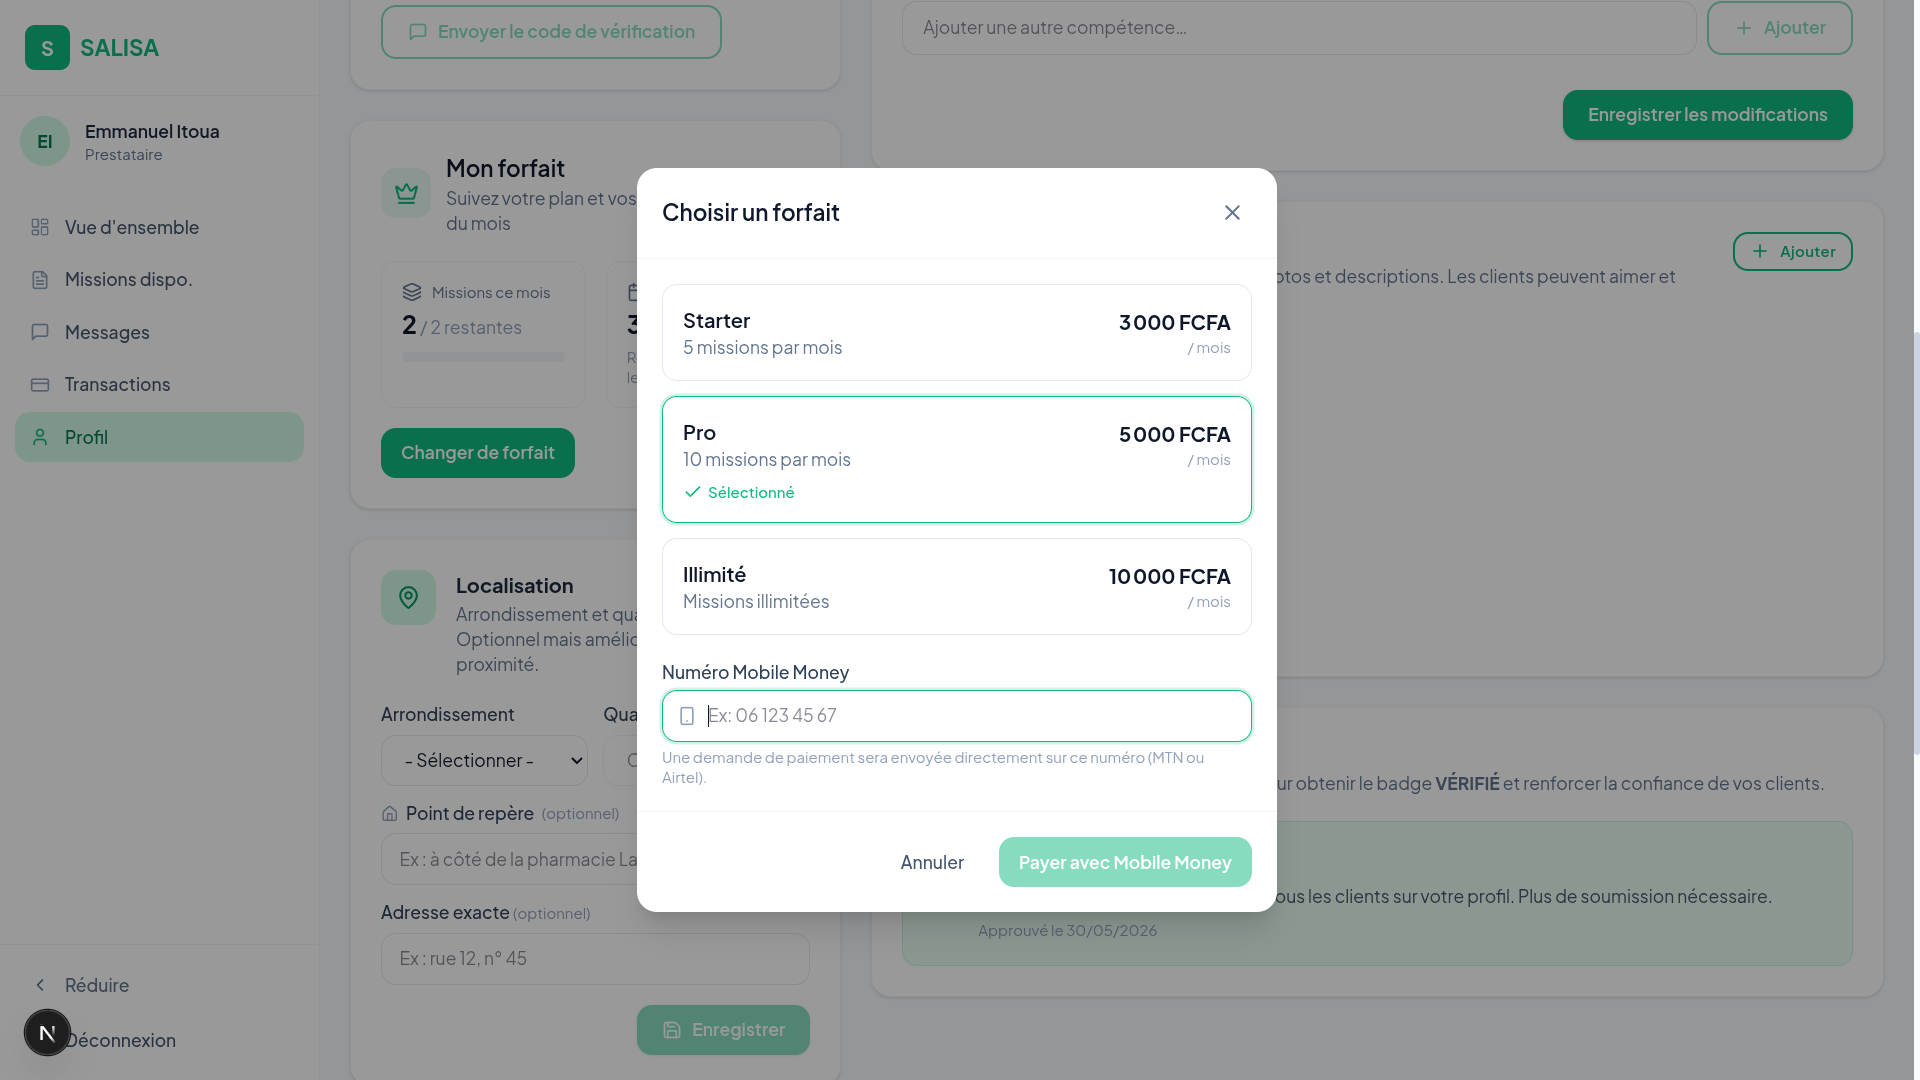
\includegraphics[width=0.85\textwidth, height=9.5cm, keepaspectratio=false]{captures_appli/capture_choix_forfait.png}
	\caption{Choix du forfait}
	\label{fig:cap_choix_forfait}
\end{figure}

\begin{figure}[H]
	\centering
	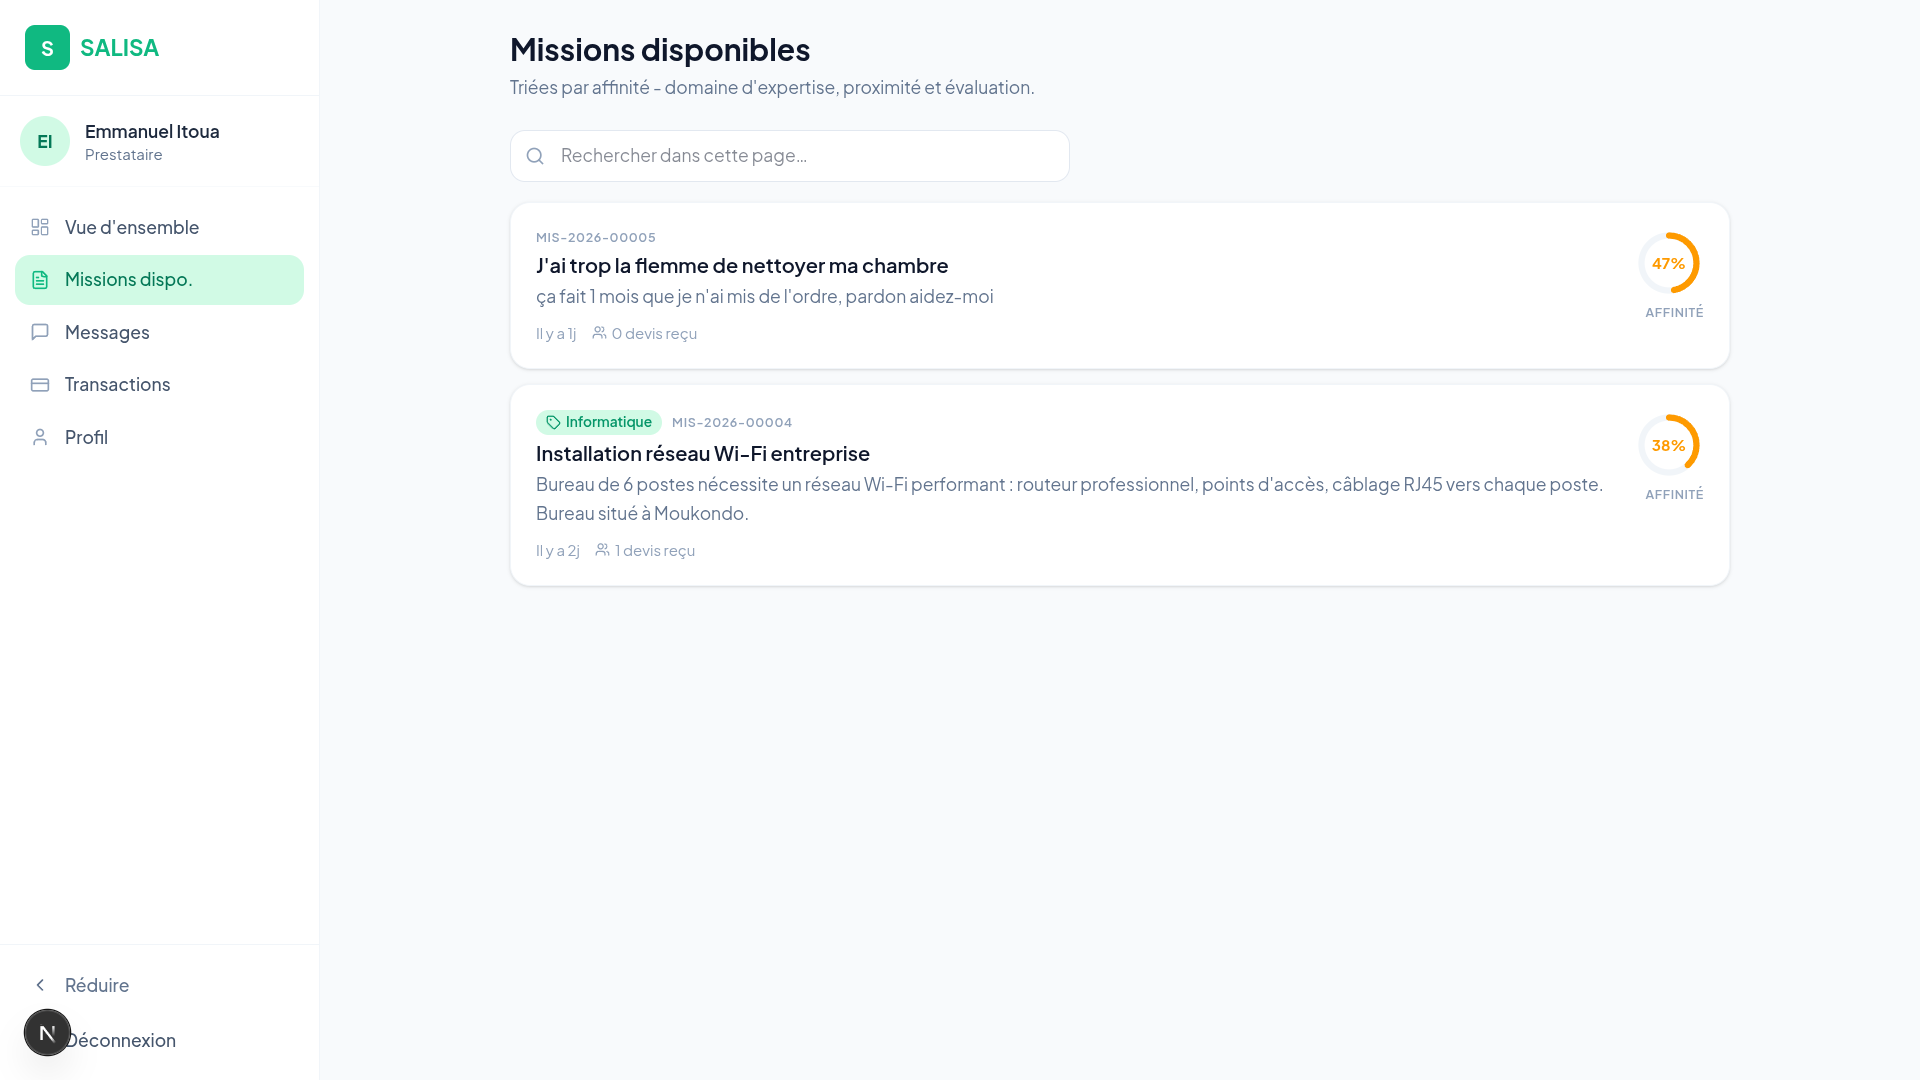
\includegraphics[width=0.85\textwidth, height=9.5cm, keepaspectratio=false]{captures_appli/capture_liste_missions.png}
	\caption{Liste des missions du prestataire}
	\label{fig:cap_liste_missions}
\end{figure}

\begin{figure}[H]
	\centering
	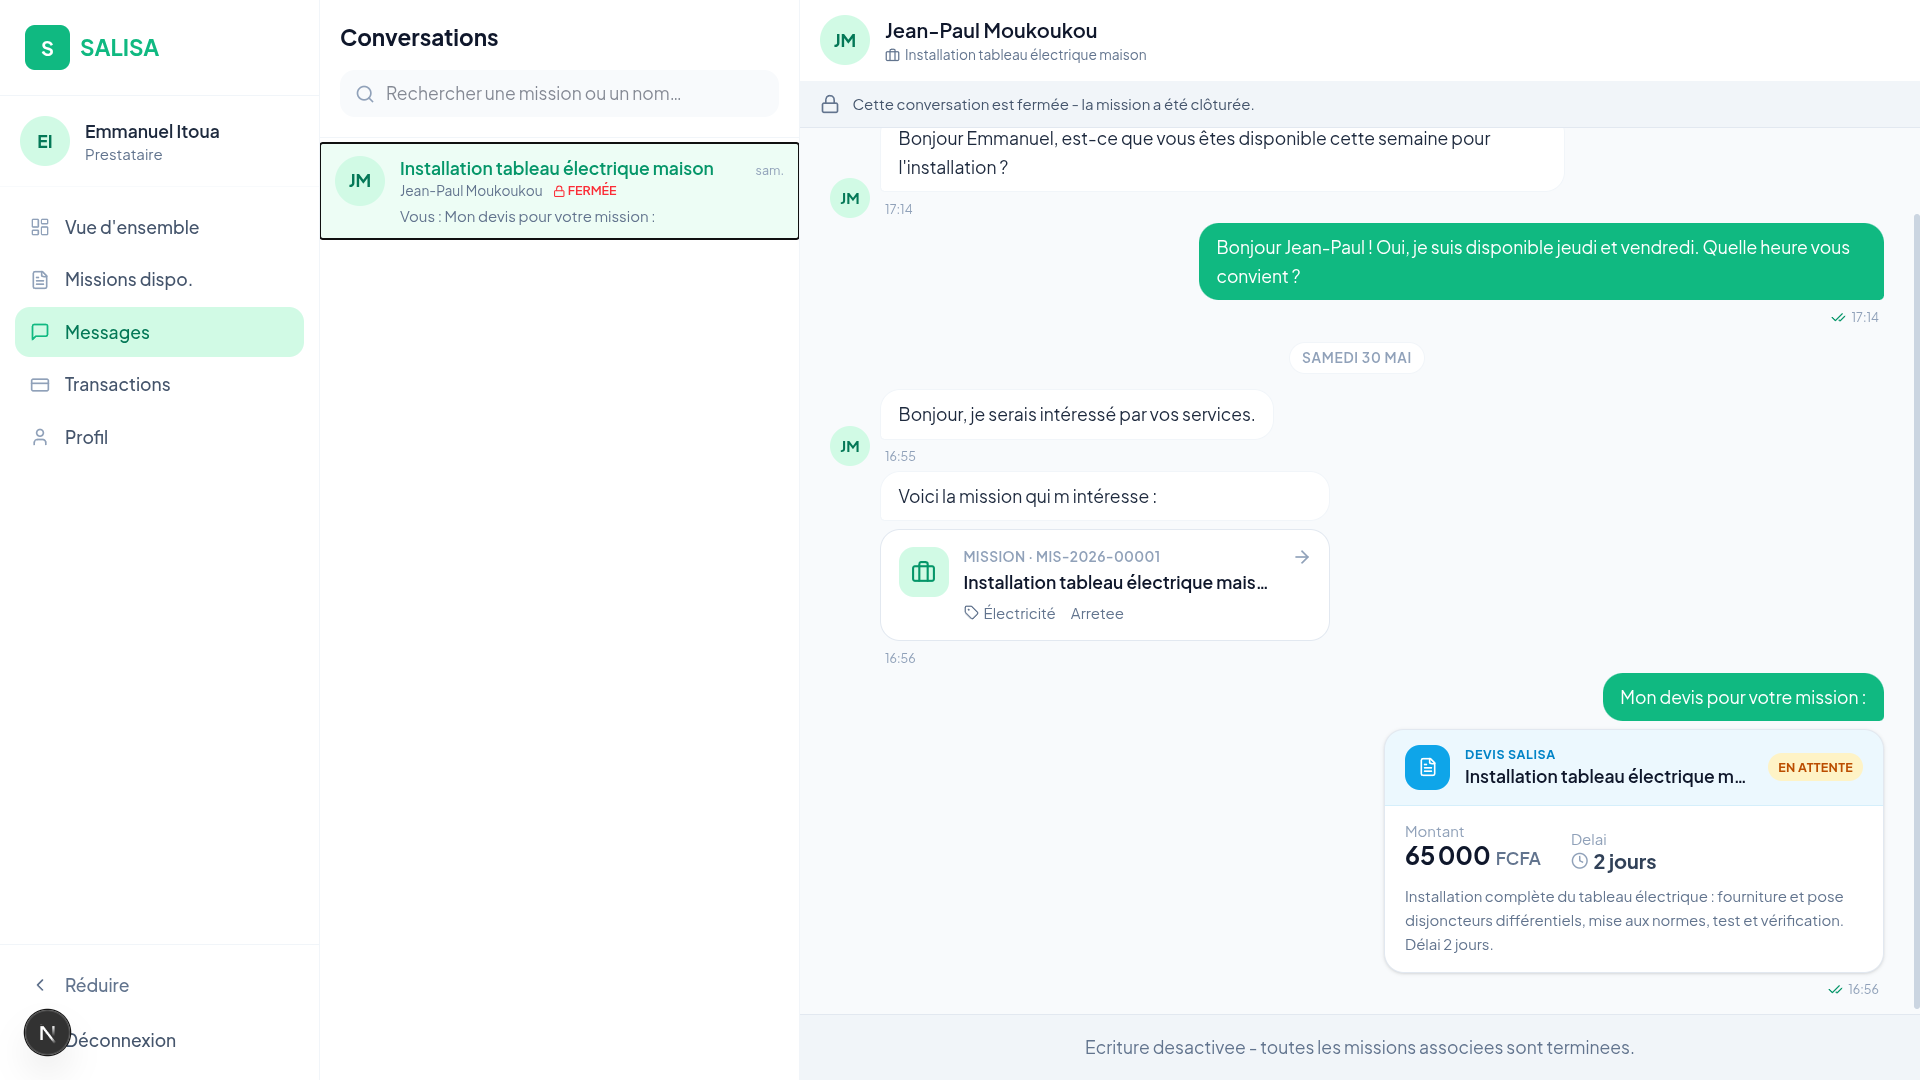
\includegraphics[width=0.85\textwidth, height=9.5cm, keepaspectratio=false]{captures_appli/capture_conversation_avec_demandeur.png}
	\caption{Discussion avec un demandeur}
	\label{fig:cap_discussion_avec_demandeur}
\end{figure}

\begin{figure}[H]
	\centering
	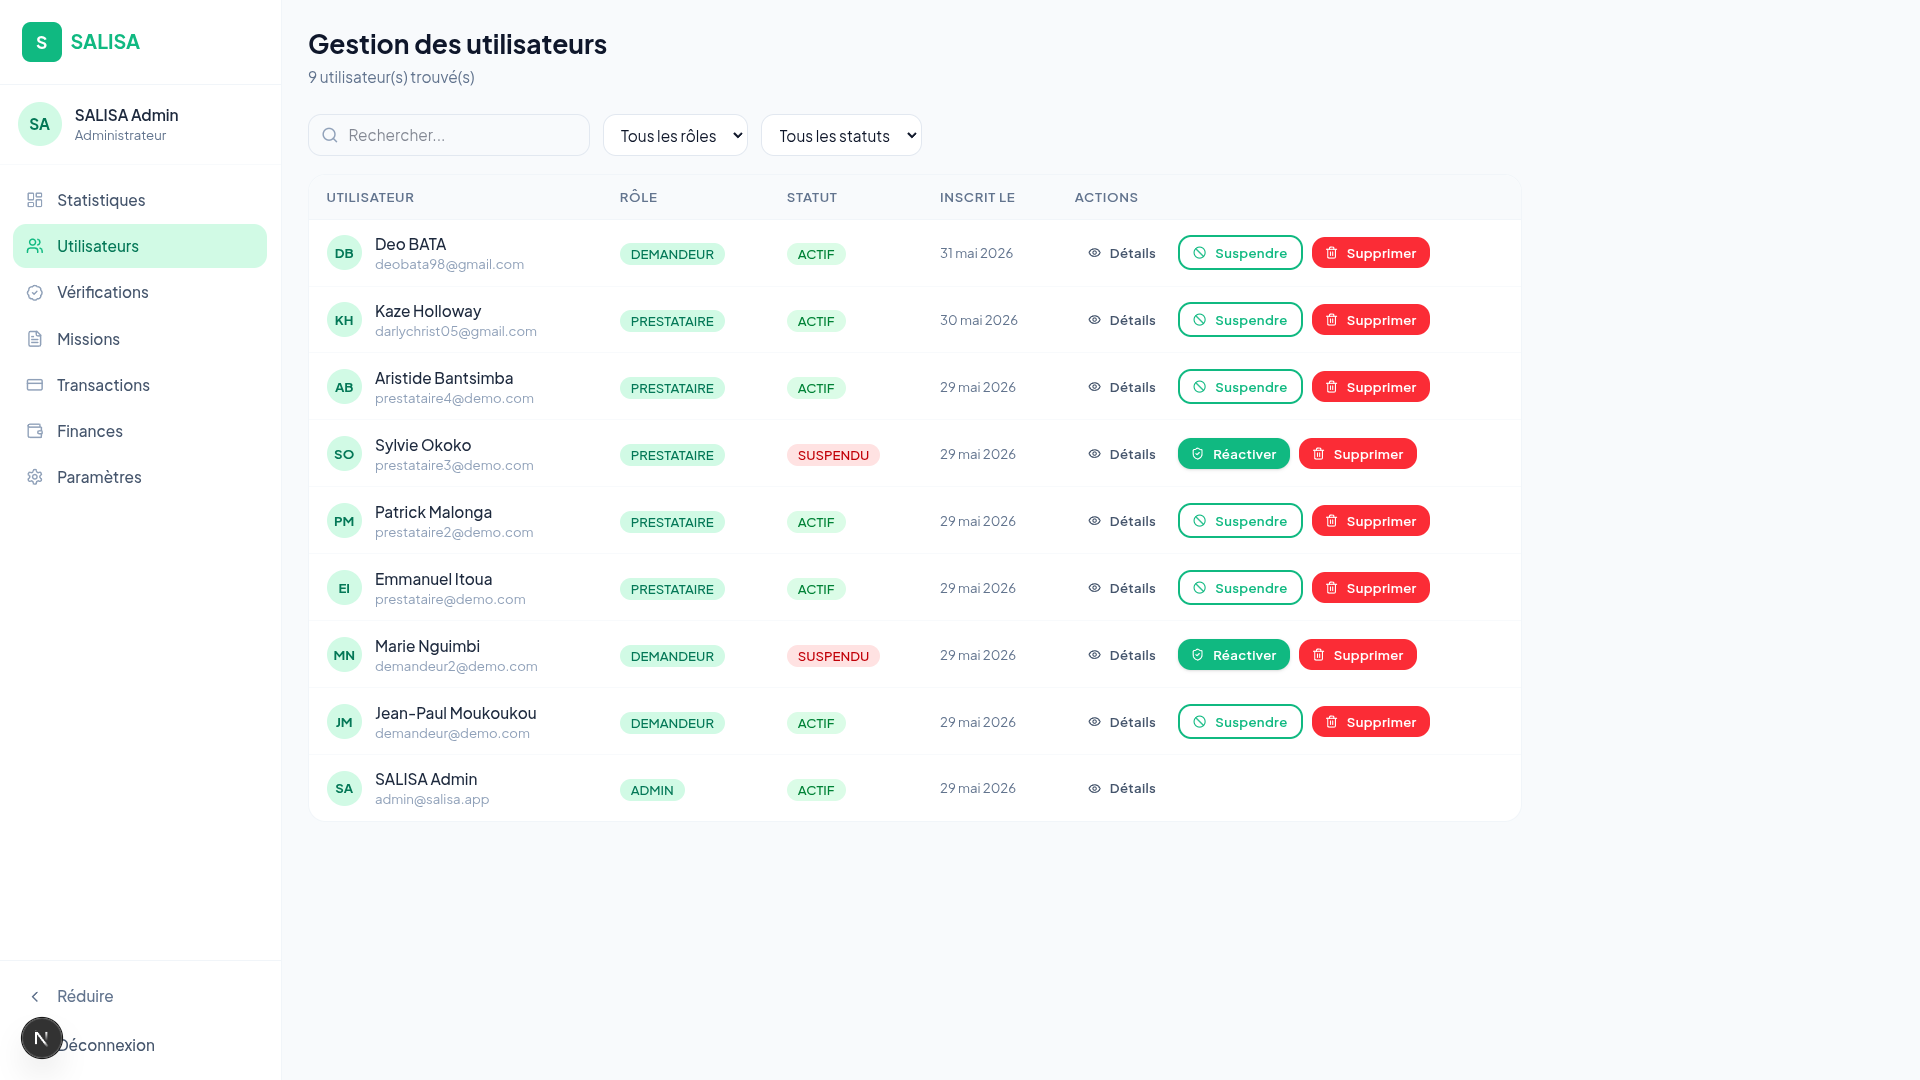
\includegraphics[width=0.85\textwidth, height=9.5cm, keepaspectratio=false]{captures_appli/capture_gestion_user.png}
	\caption{Gestion des utilisateurs}
	\label{fig:cap_gestion_user}
\end{figure}

\begin{figure}[H]
	\centering
	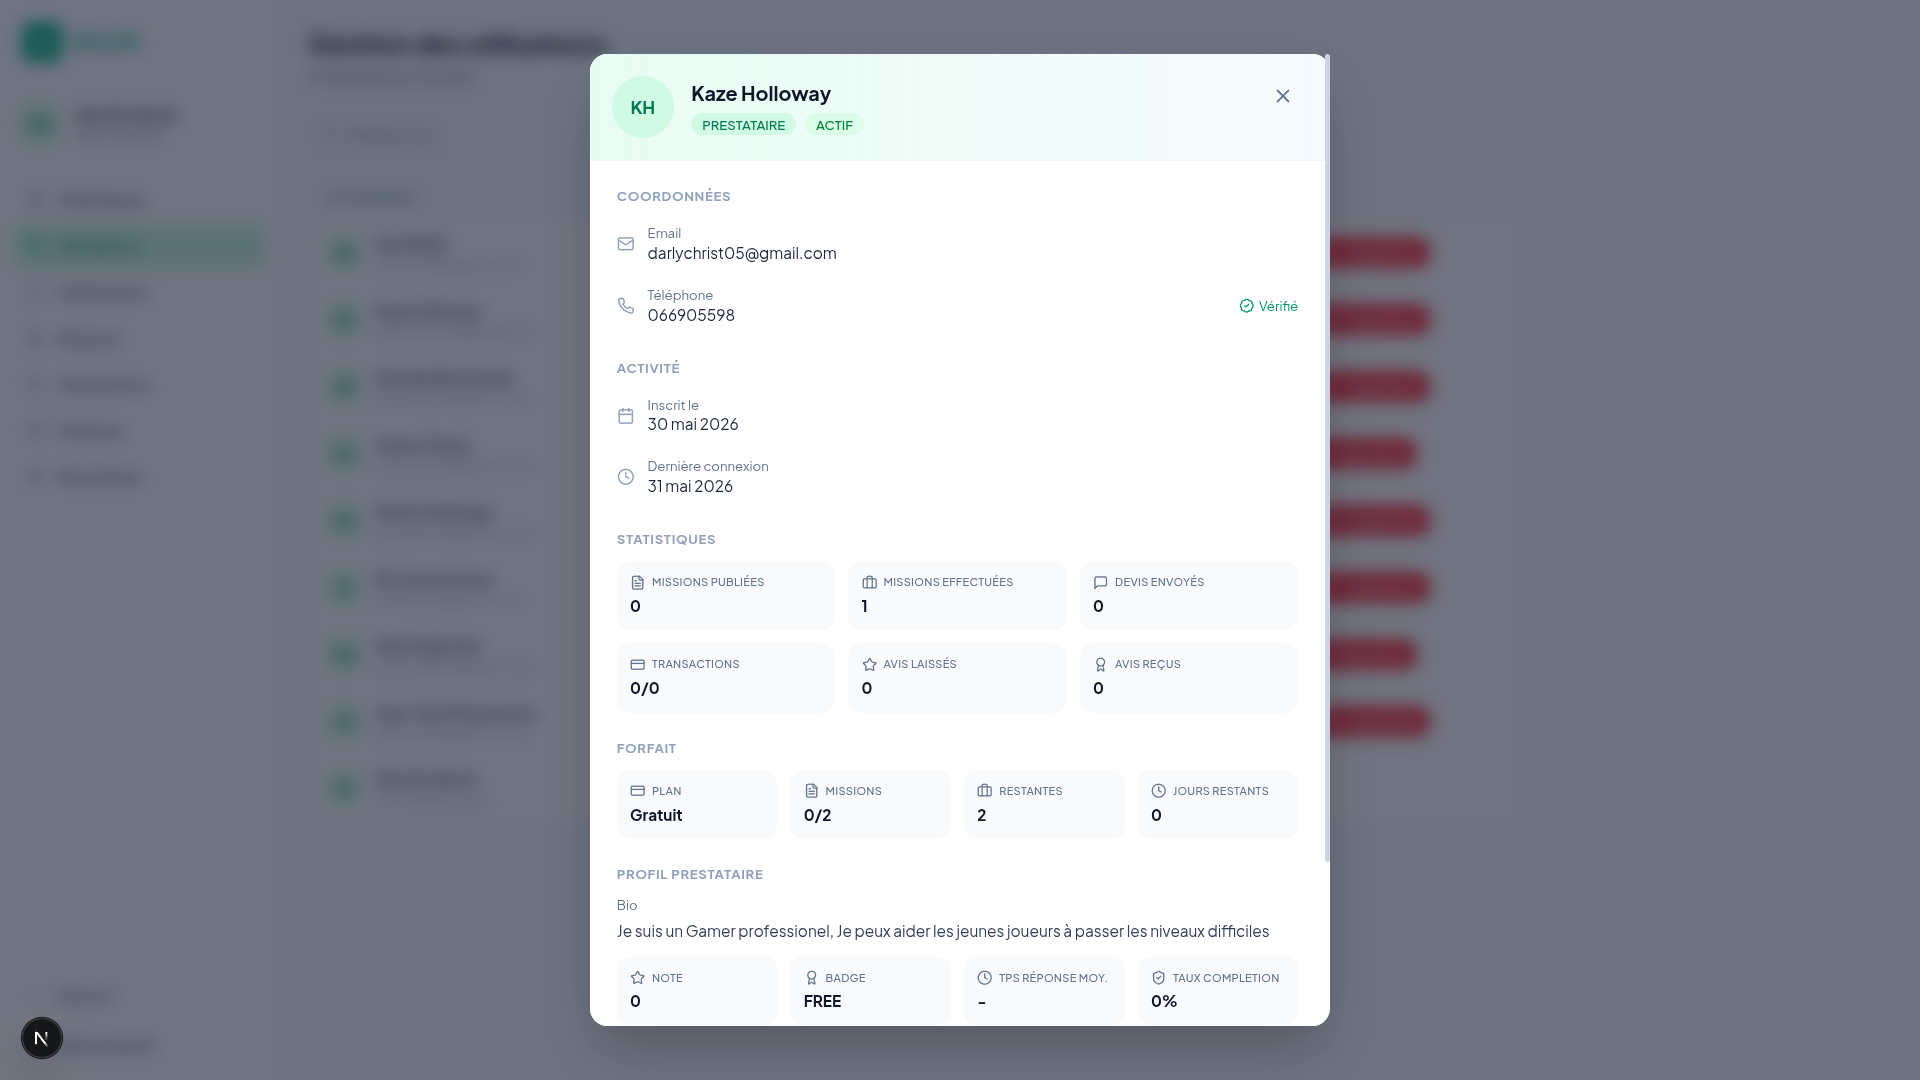
\includegraphics[width=0.85\textwidth, height=9.5cm, keepaspectratio=false]{captures_appli/capture_detail_compte.png}
	\caption{Détails d'un compte utilisateur}
	\label{fig:cap_detail_user}
\end{figure}

\begin{figure}[H]
	\centering
	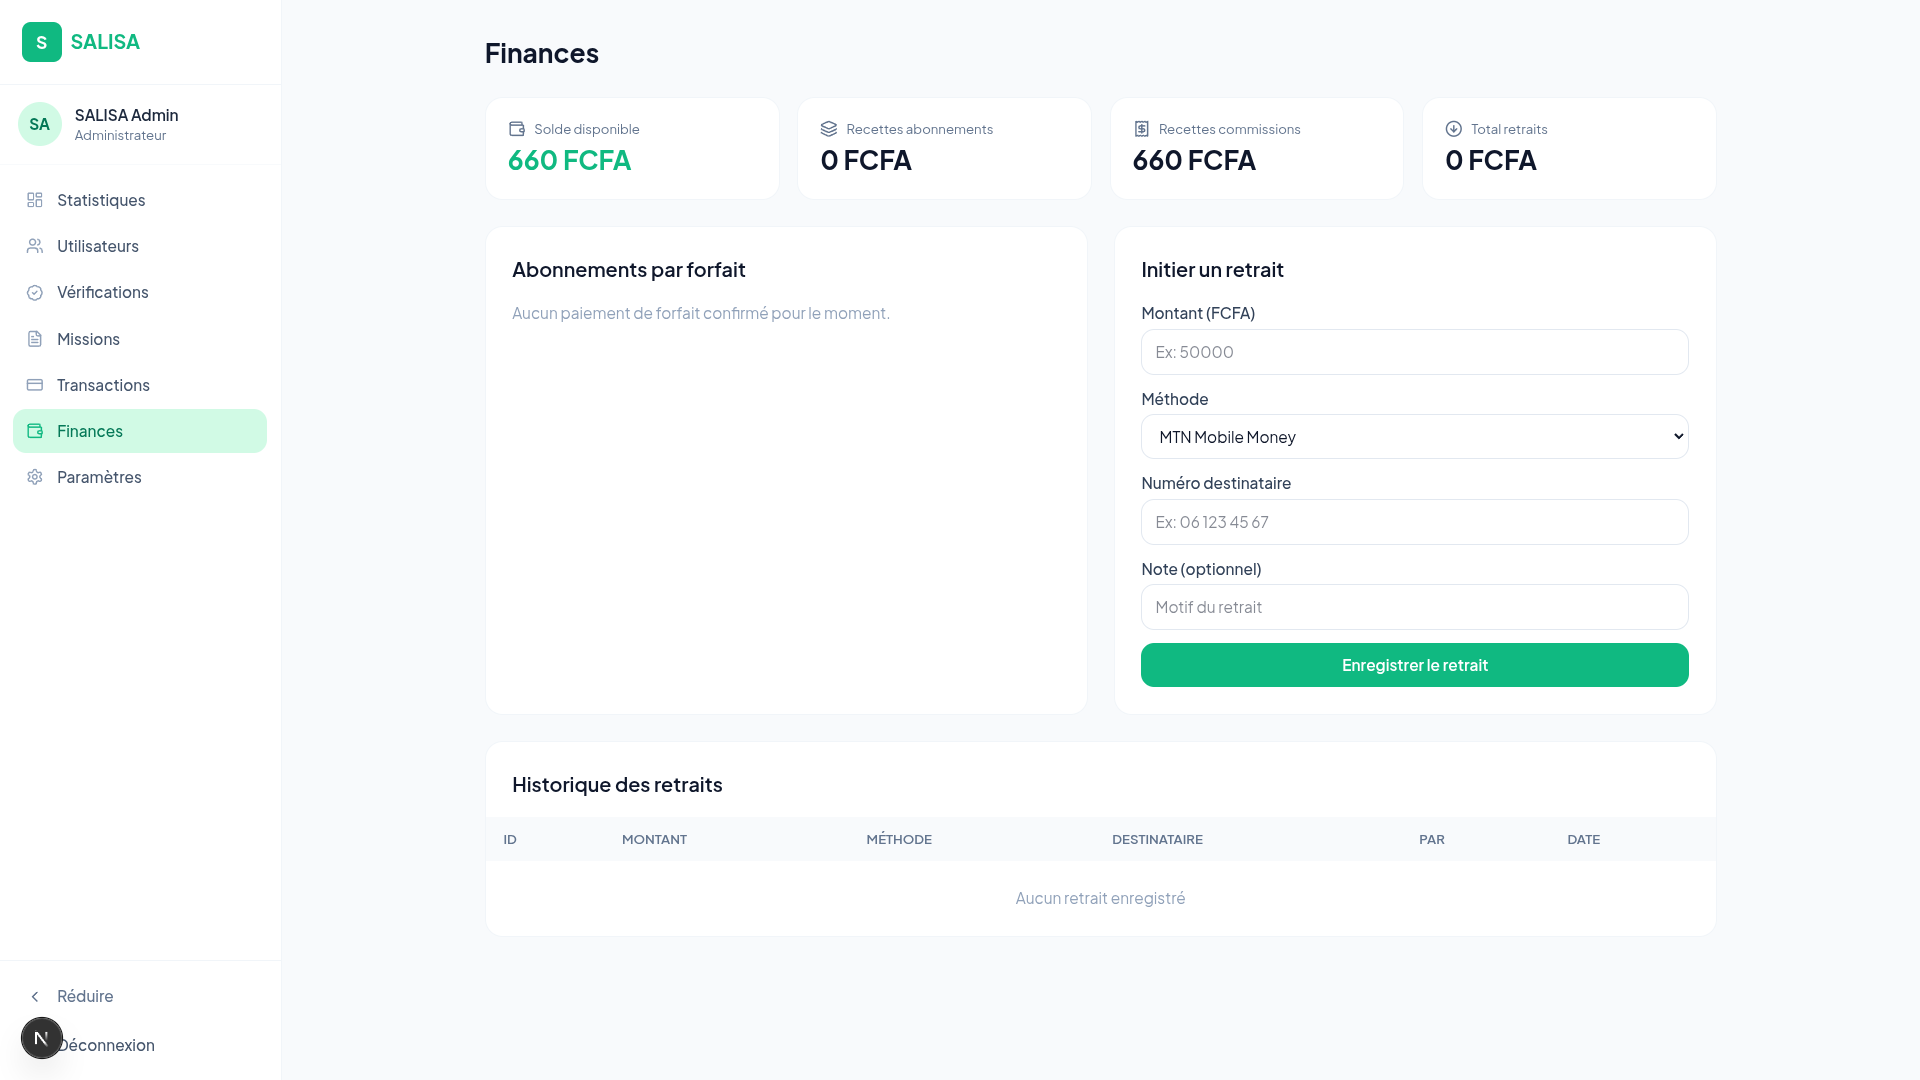
\includegraphics[width=0.85\textwidth, height=9.5cm, keepaspectratio=false]{captures_appli/capture_gestion_finance.png}
	\caption{Gestion des finances}
	\label{fig:cap_finance}
\end{figure}

\begin{figure}[H]
	\centering
	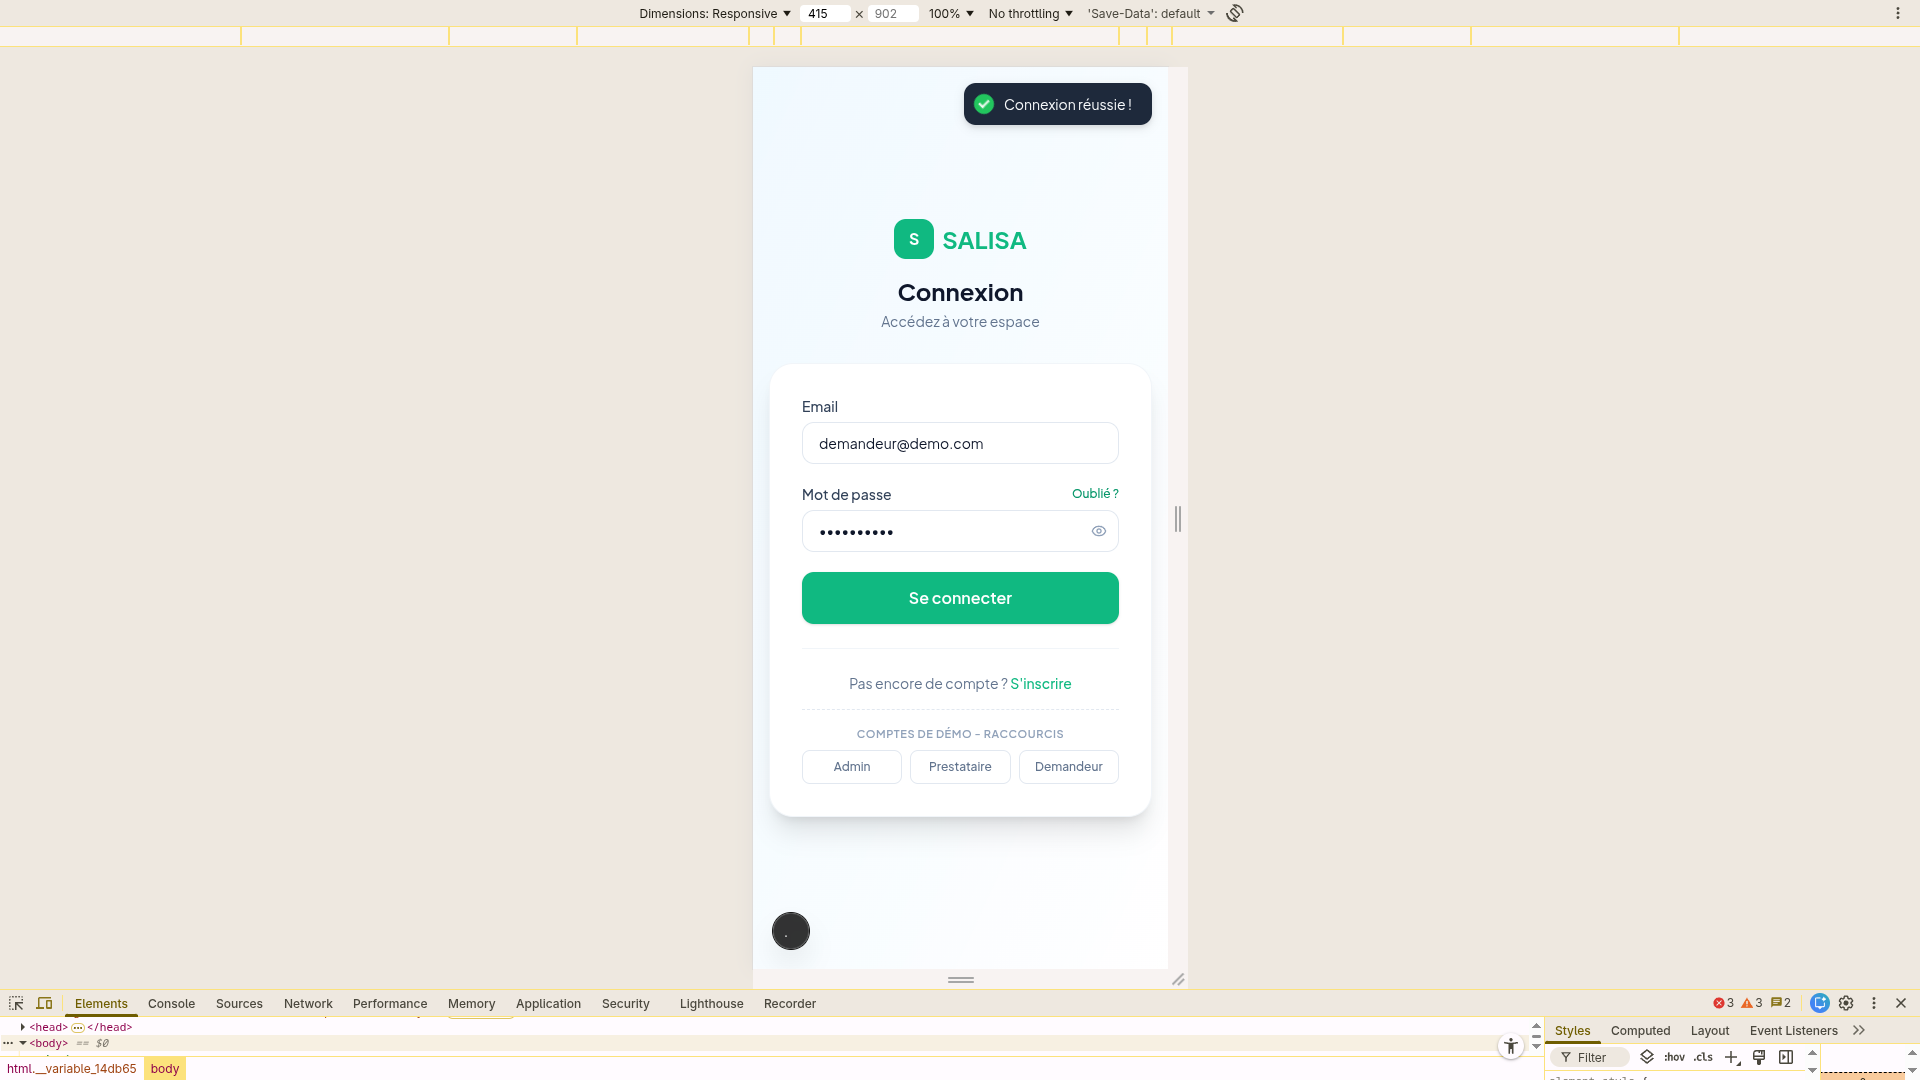
\includegraphics[width=0.85\textwidth, height=9.5cm, keepaspectratio=false]{captures_appli/capture_connexion_sur_mobile.png}
	\caption{Page de connexion (vue mobile)}
	\label{fig:cap_connexion_mobile}
\end{figure}

\begin{figure}[H]
	\centering
	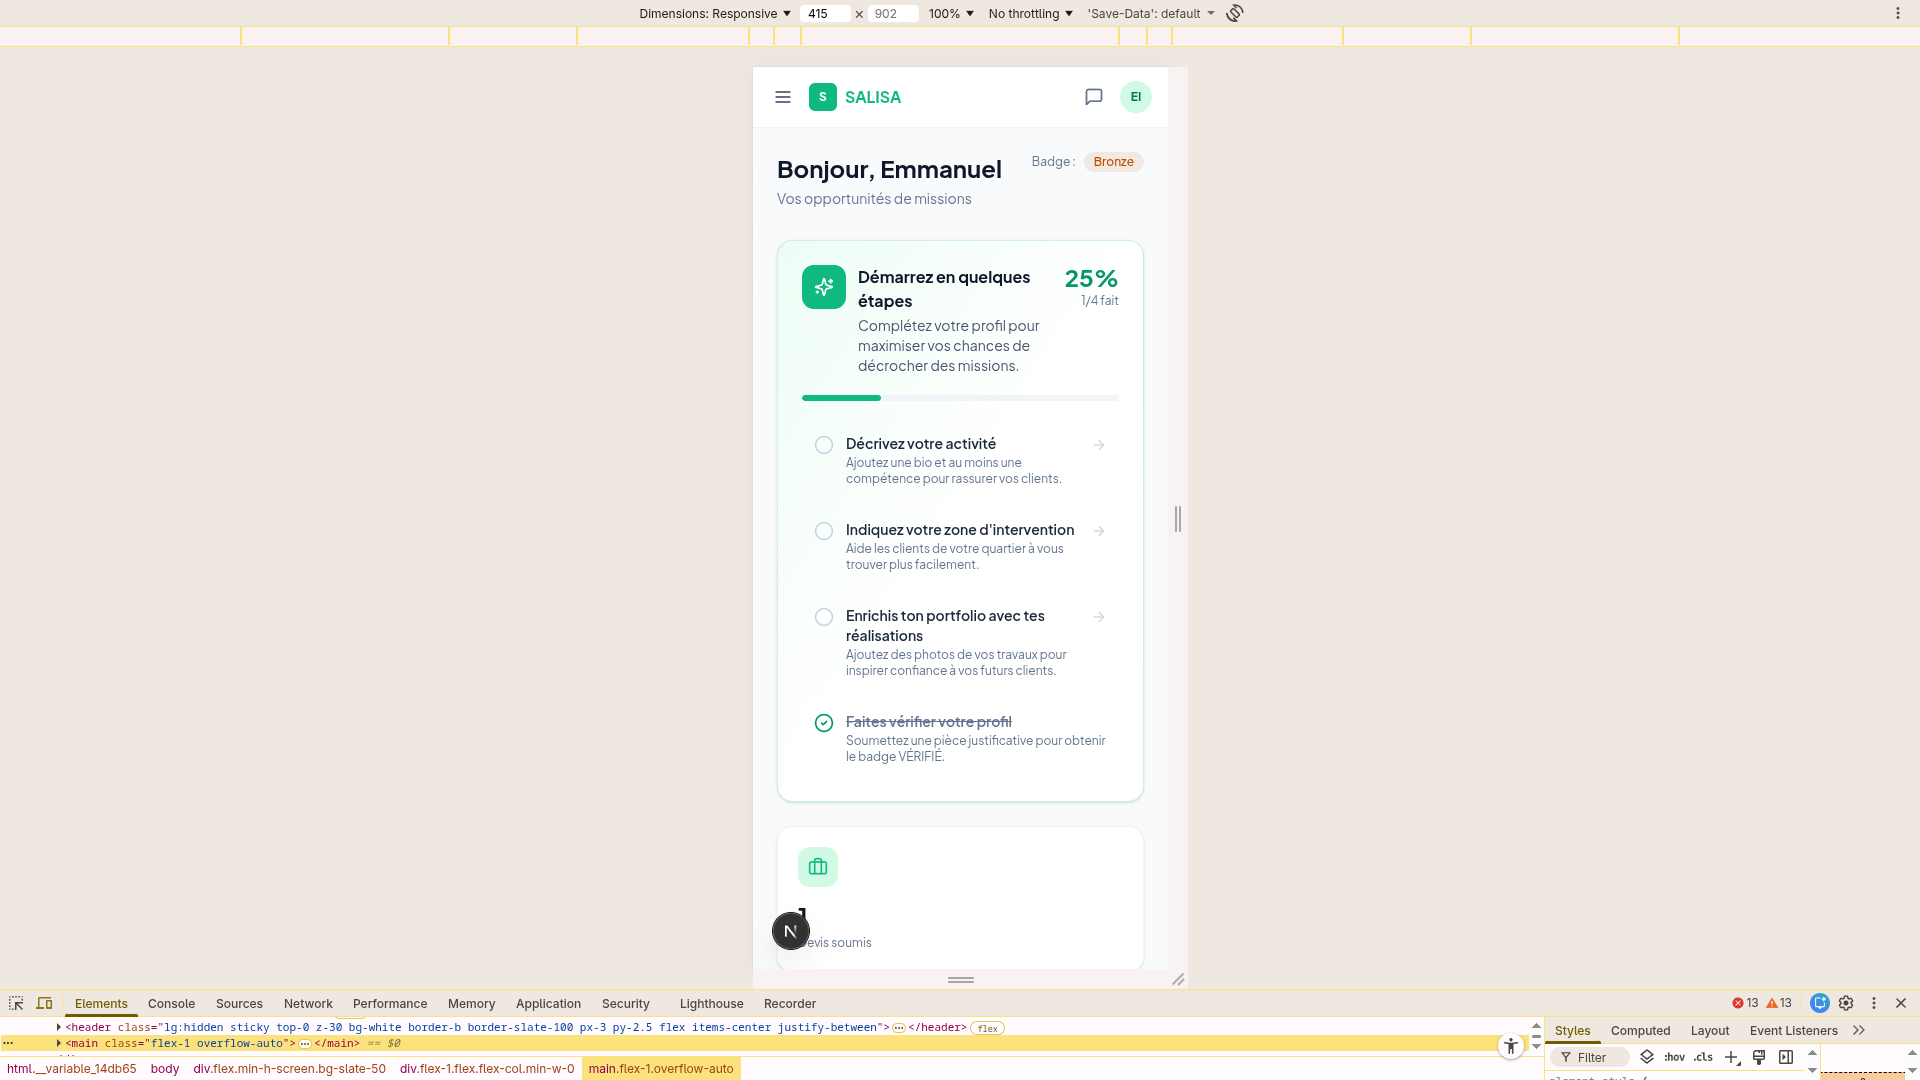
\includegraphics[width=0.85\textwidth, height=9.5cm, keepaspectratio=false]{captures_appli/capture_completion_profil_prestataire_mobile.png}
	\caption{Complétion profil prestataire (vue mobile)}
	\label{fig:cap_complete_profil_mobile}
\end{figure}

\begin{figure}[H]
	\centering
	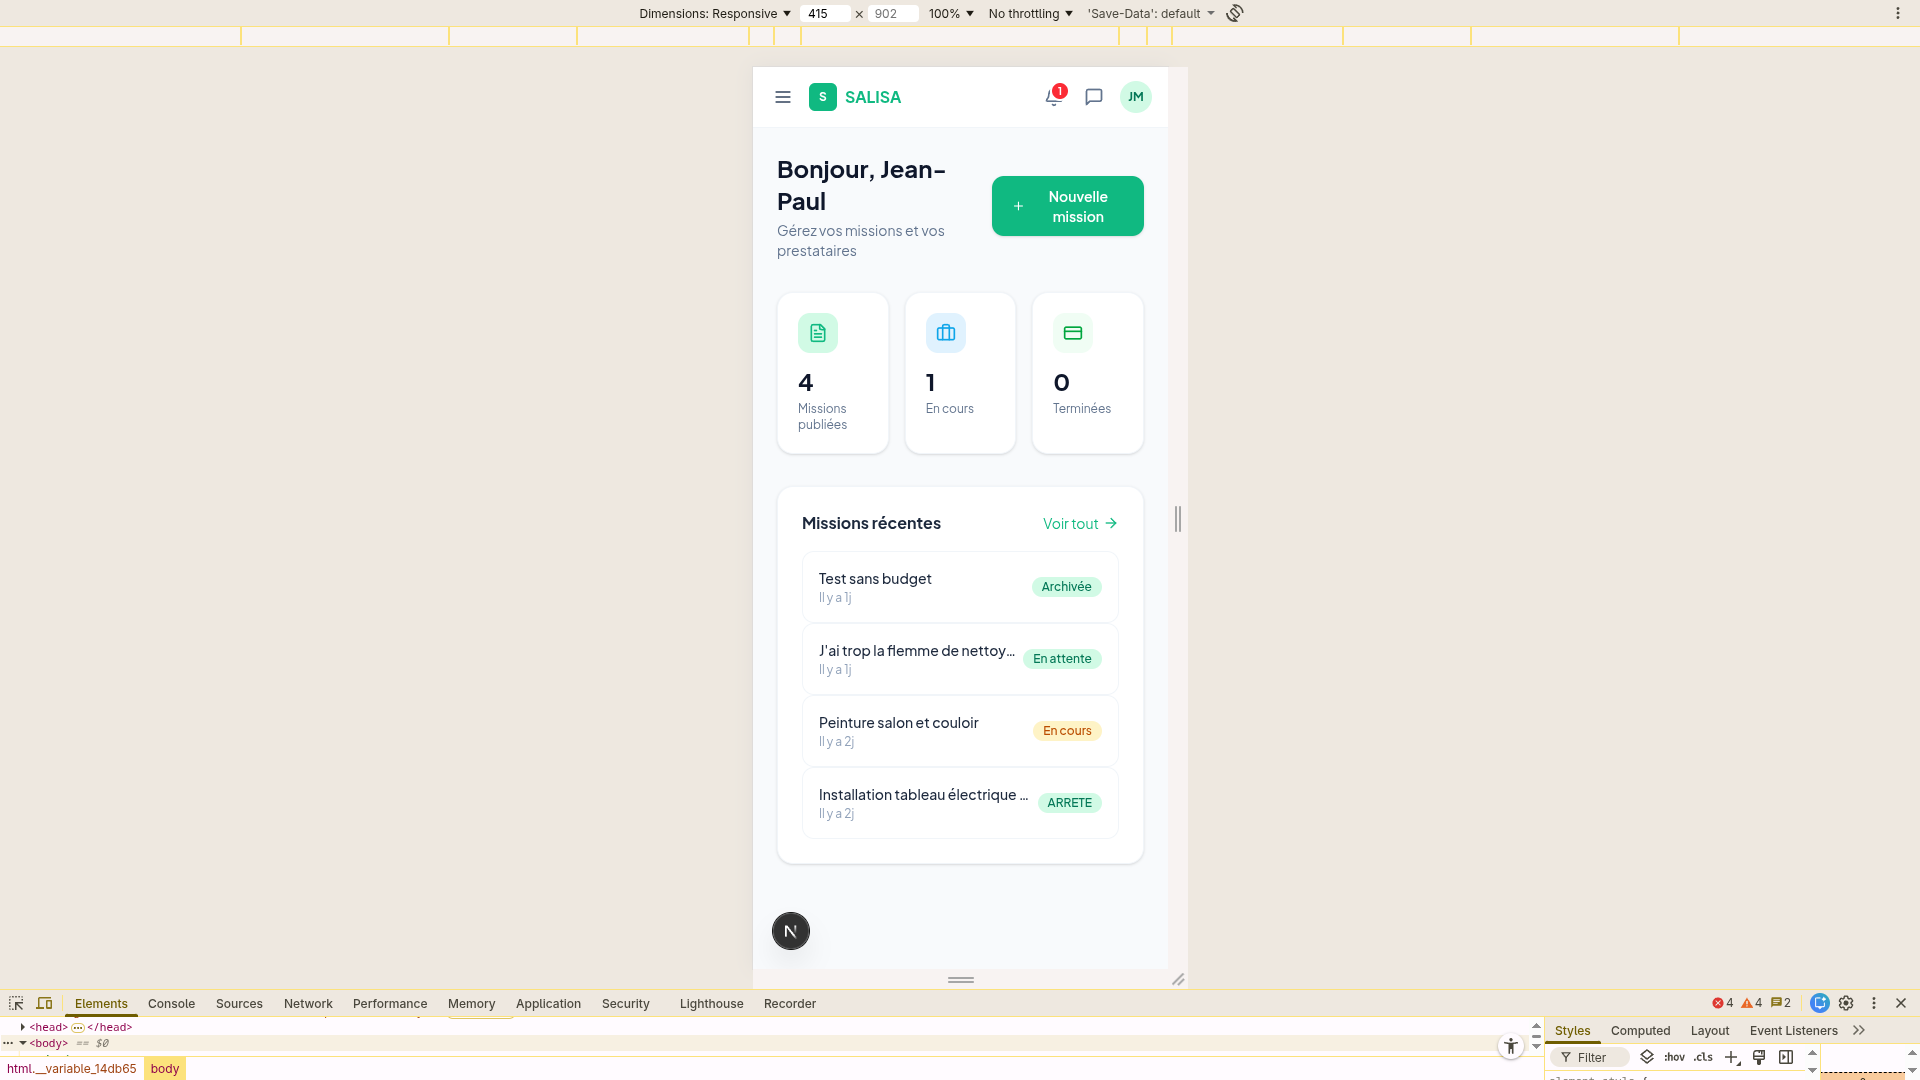
\includegraphics[width=0.85\textwidth, height=9.5cm, keepaspectratio=false]{captures_appli/capture_dashboard_demandeur_mobile.png}
	\caption{Tableau de bord demandeur (vue mobile)}
	\label{fig:cap_dashboard_demandeur_mobile}
\end{figure}


\begin{figure}[H]
	\centering
	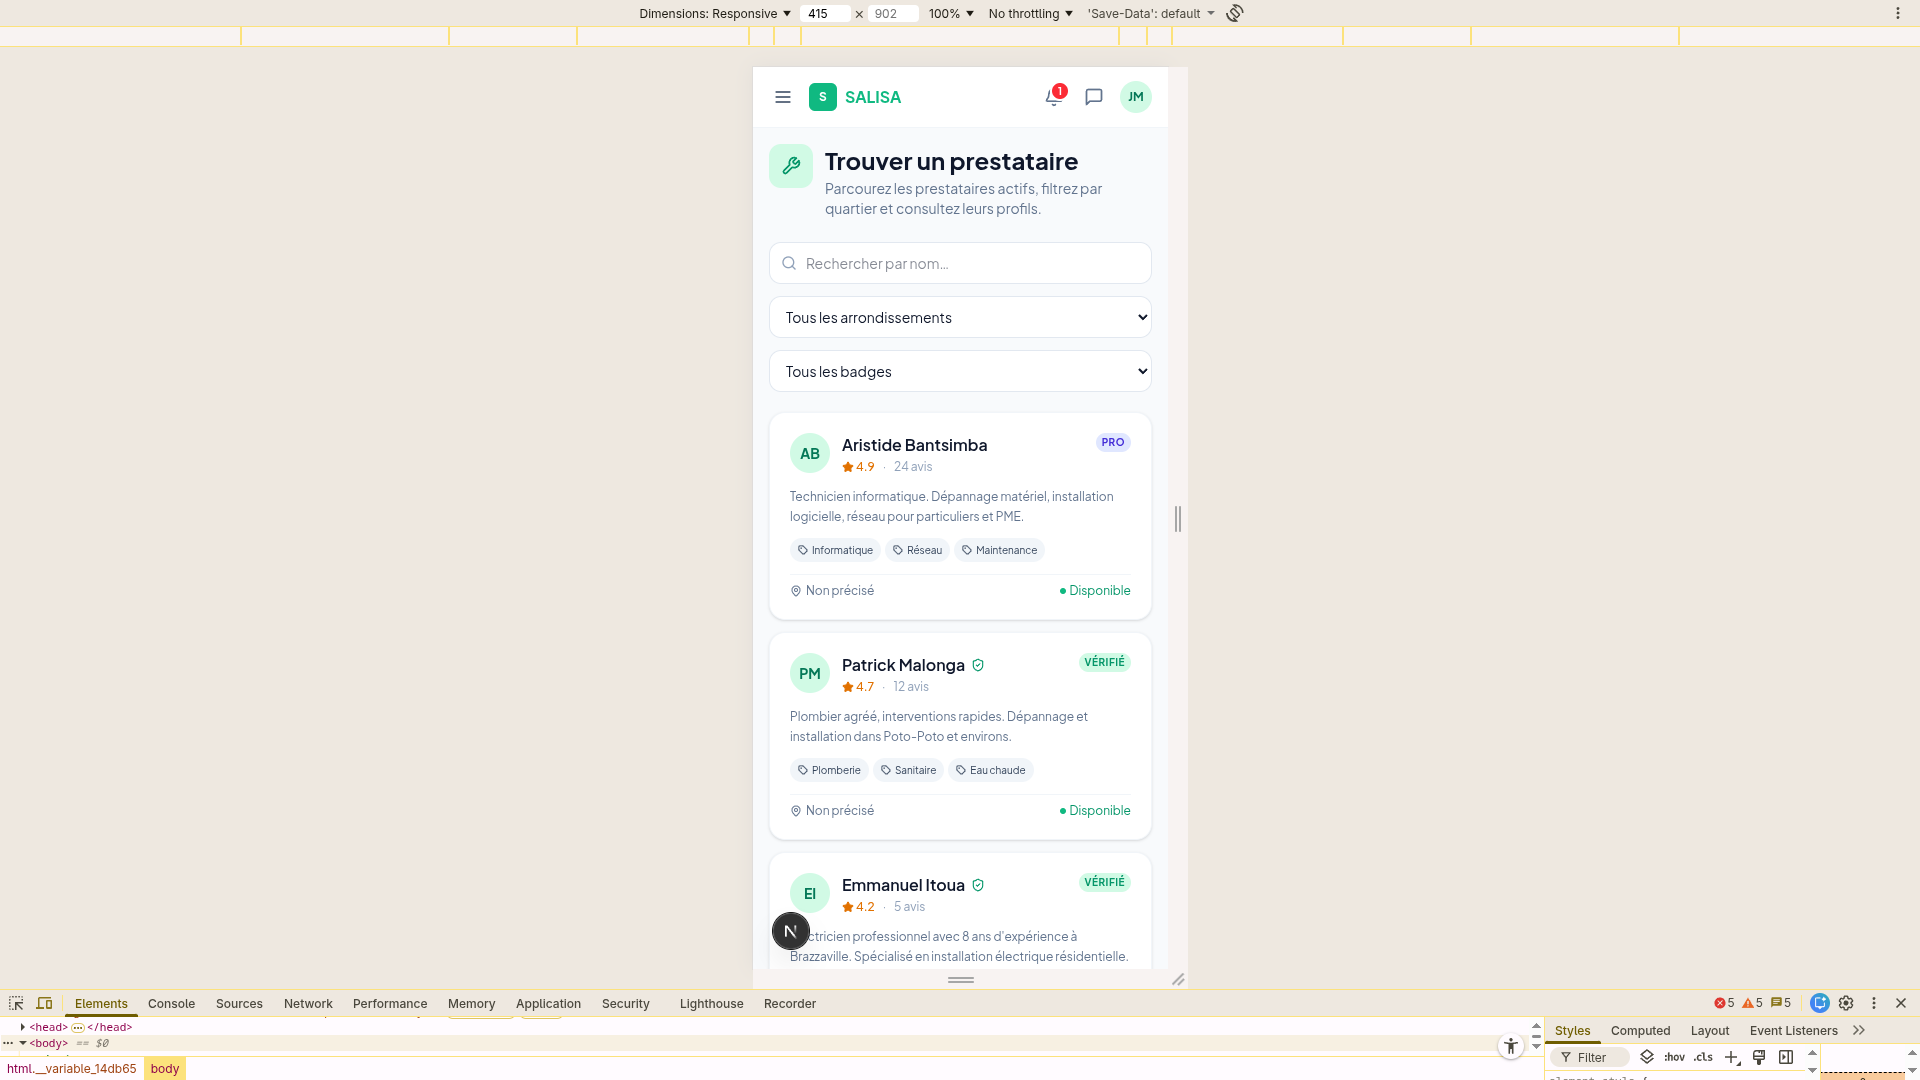
\includegraphics[width=0.85\textwidth, height=9.5cm, keepaspectratio=false]{captures_appli/capture_recherche_prestataire_mobile.png}
	\caption{Recherche prestataire (vue mobile)}
	\label{fig:cap_recherche_prestataire_mobile}
\end{figure}

\begin{figure}[H]
	\centering
	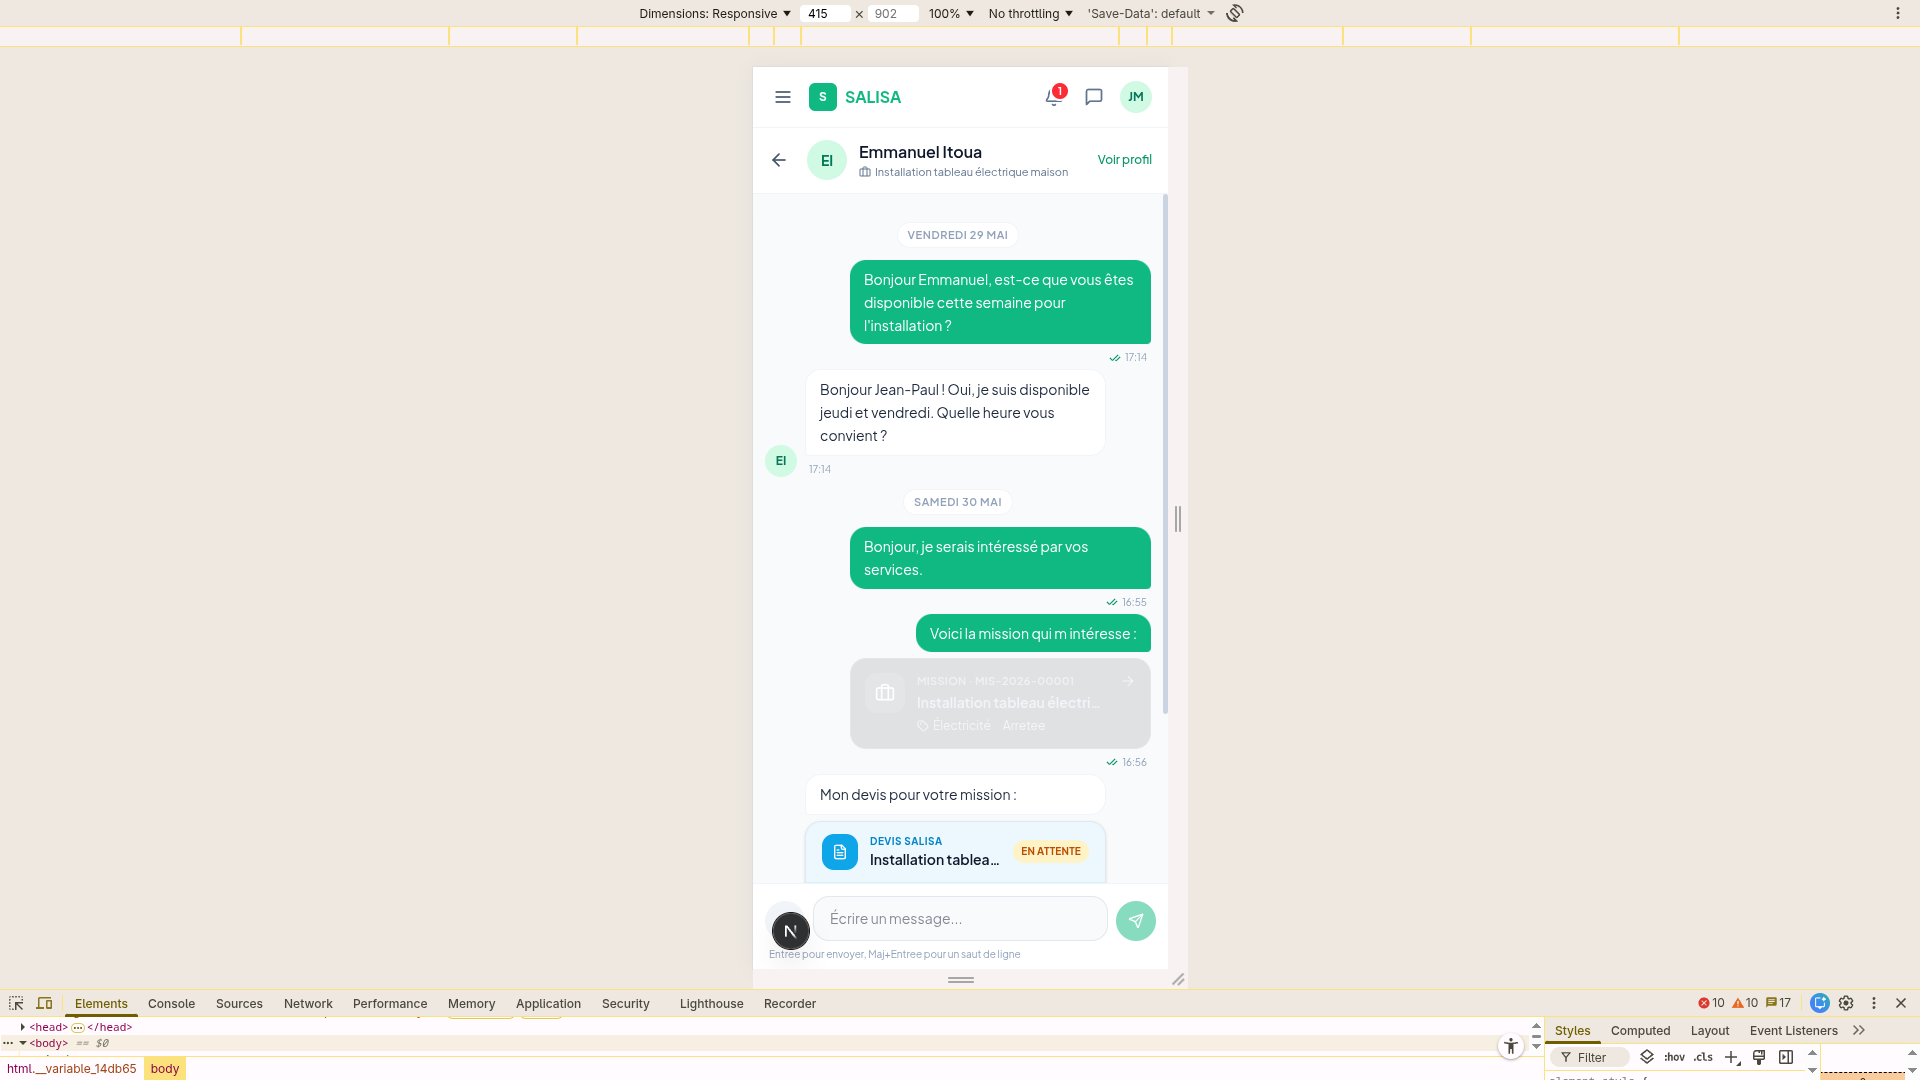
\includegraphics[width=0.85\textwidth, height=9.5cm, keepaspectratio=false]{captures_appli/capture_discute_avec_prestataire_mobile.png}
	\caption{Discussion avec un prestataire (vue mobile)}
	\label{fig:cap_discussion_avec_prestatire_mobile}
\end{figure}

	
	% ============================================================
% CONCLUSION
% ============================================================
\chapter*{Conclusion}
\pagestyle{styleGlobal}
\label{sec:conclusion}
\markboth{Conclusion}{Conclusion}
\addcontentsline{toc}{chapter}{Conclusion}

Au terme de ce travail, nous avons conçu et réalisé «~SALISA~», une application cross-plateforme de mise en relation entre prestataires et clients pour services professionnels, développée pour le compte d'Akieni.

Ce travail nous a permis de parcourir l'ensemble du cycle de développement logiciel, depuis l'analyse des besoins jusqu'à la réalisation d'une solution fonctionnelle, en passant par la conception architecturale et la modélisation UML selon la démarche \textbf{2TUP}. Nous avons pu mesurer concrètement la complémentarité entre un langage de modélisation expressif comme UML et un processus de développement structuré comme le 2TUP, dont l'approche en deux branches parallèles s'est révélée particulièrement adaptée à la complexité de «~SALISA~».

Sur le plan fonctionnel, «~SALISA~» propose un ensemble de fonctionnalités répondant aux besoins réels du marché congolais : mise en correspondance intelligente entre prestataires et demandeurs, système de confiance à plusieurs niveaux, paiement sécurisé par Mobile Money via un mécanisme d'escrow, messagerie en temps réel et notifications multi-canaux. L'application est conçue comme une \textit{Progressive Web Application} (PWA), optimisée pour les réseaux mobiles et accessible sans installation.

Ce travail illustre la capacité du numérique à structurer des marchés informels et à créer de la valeur économique locale, tout en répondant aux contraintes spécifiques du contexte africain. Il constitue une contribution concrète à la transformation numérique en cours en République du Congo.

En perspective, plusieurs axes d'amélioration pourront être envisagés : le déploiement d'un module de machine learning pour affiner l'algorithme de mise en correspondance, l'extension de «~SALISA~» vers d'autres villes du pays comme Pointe-Noire, le développement d'une application mobile native, et la mise en place d'un programme d'ambassadeurs pour accélérer son adoption.

Ce travail, mené dans le cadre de notre formation en Licence Professionnelle Génie Logiciel à l'ESGAE, nous a permis de consolider nos compétences techniques et méthodologiques, tout en relevant un défi concret ancré dans les réalités de notre pays.

\vspace{1cm}
\begin{flushright}
    \textit{Ko salisa biso nyonso} - Nous nous entraidons tous.
\end{flushright}

	
	% ============================================================
	% SECTION III
	% ============================================================
	\pageSectionAnnonce{SECTION III}
	\pagenumbering{alph}
	\addtocontents{toc}{%
		\vspace{10pt}%
		\noindent{\fontsize{13}{16}\selectfont\bfseries SECTION III}\par%
		\vspace{3pt}%
	}
	
	\phantomsection
	\label{sec:tabledesmatieres}
	\addcontentsline{toc}{chapter}{Table des matières}
	\renewcommand{\contentsname}{\textcolor{vertCongo}{Table des matières}}
	\tableofcontents
	\newpage
	
	\phantomsection
	\label{sec:bibliographie}
	\addcontentsline{toc}{chapter}{Bibliographie}
	\bibliographystyle{plain}
	\nocite{*}
	\bibliography{biblio}
	\newpage
	
	\appendix
	% ============================================================
% ANNEXES
% ============================================================
\chapter*{Annexes}
\pagestyle{styleGlobal}
\label{sec:annexes}
\markboth{Annexes}{Annexes}
\addcontentsline{toc}{chapter}{Annexes}

\vspace*{0.5cm}

\section*{Annexe A : Schéma de la base de données (Prisma)}

Le schéma ci-dessous représente la définition complète de la base de données de « SALISA », telle qu'elle a été implémentée avec l'outil Prisma ORM. Il traduit directement le diagramme de classes présenté dans la partie Analyse et Conception et sert de référence technique pour la génération des modèles de données dans l'application.

\begin{figure}[H]
	\centering
	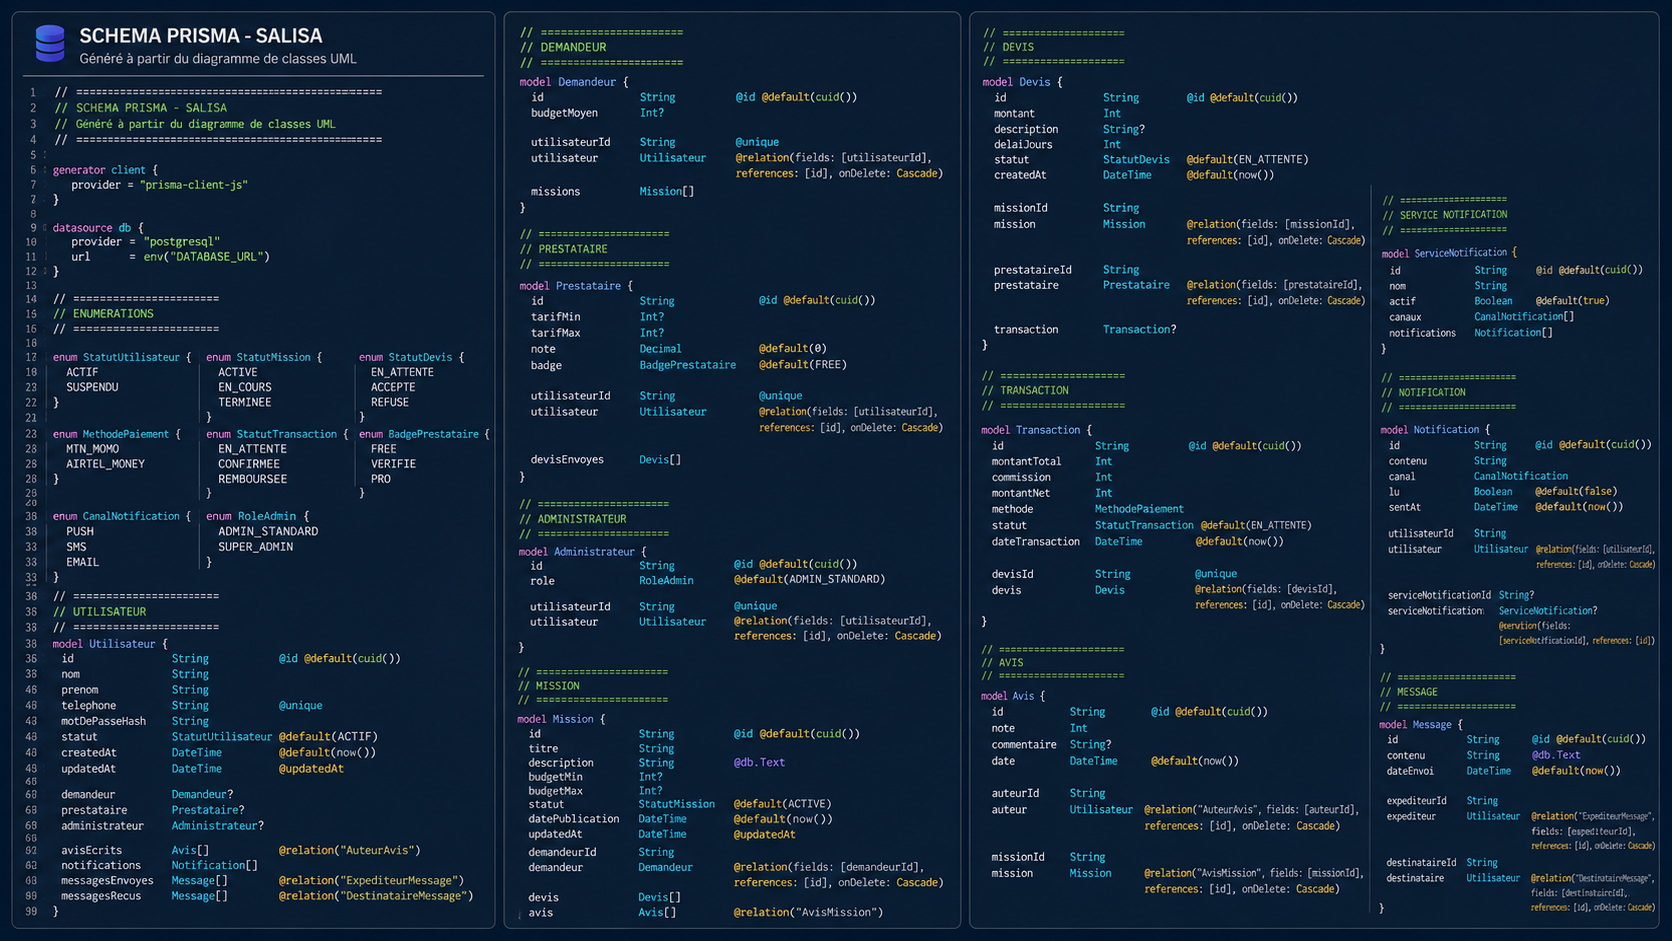
\includegraphics[width=0.95\textwidth]{schema_prisma.png}
	\caption{Schéma Prisma de la base de données de « SALISA »}
	\label{fig:schema_prisma}
\end{figure}

\section*{Annexe B : Organigramme original d'Akieni}

La figure suivante présente l'organigramme original fourni par la structure d'accueil Akieni, tel qu'il nous a été transmis. Il a servi de base à la rédaction de la section 1.1.3 du présent document.

\begin{figure}[H]
	\centering
	
\includegraphics[width=0.85\textwidth]{organigramme_original_akieni.jpg}
	\caption{Organigramme original d'Akieni (document interne)}
	\label{fig:organigramme_original}
\end{figure}
	
\end{document}